\chapter{Experimentos e análises de resultados} 
\label{cp:8_Res_exp}

Este capítulo possui como objetivo apresentar as bases de dados utilizadas nos experimentos, suas especificidades e alterações. Como também apresentar algumas estratégias de pré-processamento das imagens, configurações de experimentos e resultados obtidos.

\section{Bases de dados}

 Neste trabalho foram utilizadas as seguintes bases dispostas de maneira pública na literatura: 
\begin{itemize}
\item (\textit{i}) \textbf{AR} \footnote{http://www2.ece.ohio-state.edu/~aleix/ARdatabase.html}, disponibilizada por \citeonline{martinez1998ar} criada pela Universidade Autônoma de Barcelona, essa base possui 2600 imagens de face frontal de 100 indivíduos (50 homens e 50 mulheres). De modo que para cada indivíduo são coletadas 26 fotos, estas, sujeitas a 13 variações de condições, dentre estas estão, diferentes expressões faciais, condições de iluminação e variações de oclusão ( com óculos de sol e cachecol).

\item (\textit{ii}) \textbf{Yale}\footnote{http://vision.ucsd.edu/content/yale-face-database}, disponibilizada por \citeonline{georghiades1997yale} criada pela Universidade da Califórnia, essa base de dados contém 165 imagens frontais de 15 pessoas, com 11 imagens de face por pessoa. Além de apresentar variações de iluminação, expressão e oclusão (baixos níveis de oclusão ocasionados por óculos de grau).
	
\end{itemize}

É importante ressaltar o número de imagens de faces não ocluídas e ocluídas nas duas bases, dessa forma a base AR é composta de 1400 imagens não ocluídas e 1200 ocluídas. Já a Yale possui 150 imagens não ocluídas e 15 ocluídas com óculos de grau, destas 15 imagens foram geradas 30 (descritas com maiores detalhes na seção \ref{subsec:pre_processamento}), somando no total 180 imagens. Na figura \ref{fig:exemplos_datasets} são apresentados exemplos de imagens das duas bases de dados.


\begin{figure}[H]
\centering
\caption{Exemplos de imagens antes de aplicar o algoritmo Viola-Jones nas duas bases de dados }
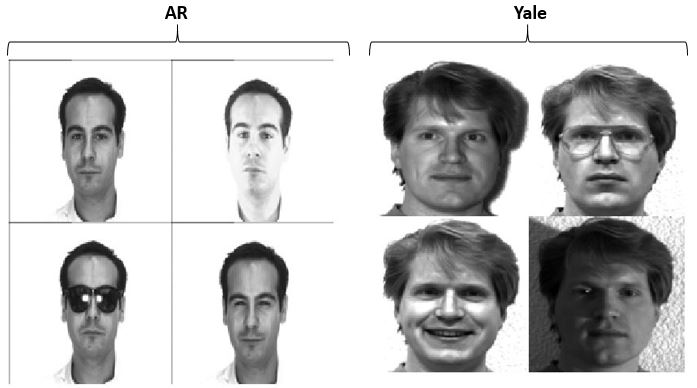
\includegraphics[scale=0.8]{imgs/exemplos_bases.png}
\source{AR \cite{martinez1998ar} e Yale \cite{georghiades1997yale}}
\label{fig:exemplos_datasets}
\end{figure}


Com o auxílio da figura \ref{fig:exemplos_variacoes_datasets} podemos visualizar as 13 variações das condições do ambiente presente na base AR.

\begin{figure}[ht]
\centering
\caption{Exemplos de variações das imagens presentes na base de dados AR }
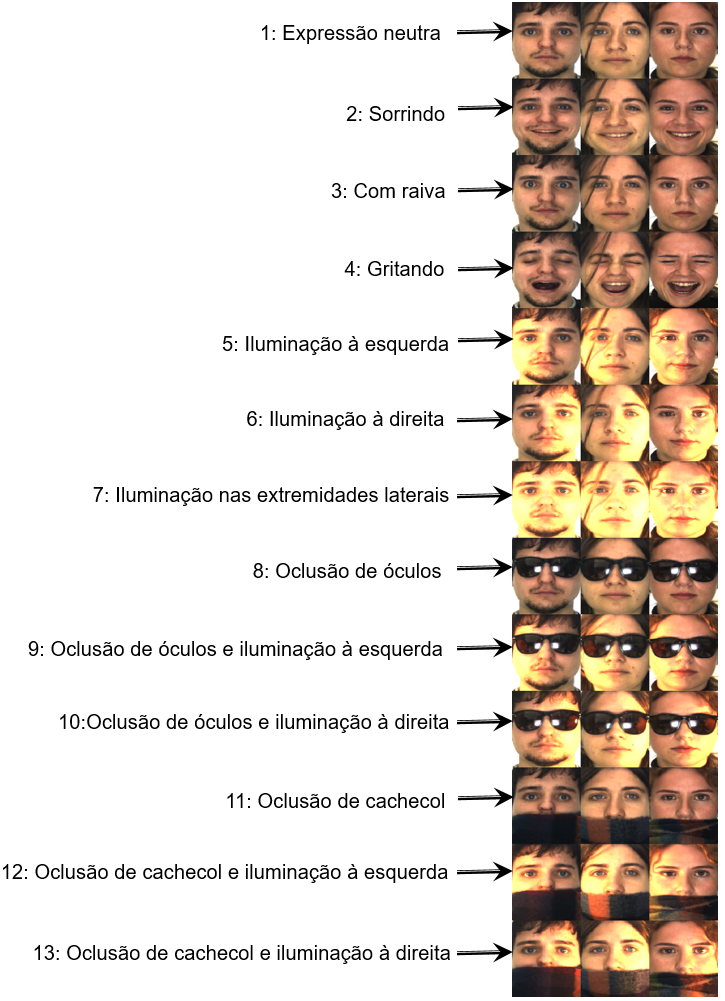
\includegraphics[scale=0.65]{imgs3/imagens_AR_ex}
\source{Jonas Mendonça Targino, 2018. Imagens de faces obtidas da base AR \cite{martinez1998ar}}
\label{fig:exemplos_variacoes_datasets}
\end{figure}




\section{Pré-processamento}
\label{subsec:pre_processamento}


Antes de tudo, todas as imagens de face foram convertidas para escala de cinza. E logo em seguida aplicado o algoritmo  Viola-Jones \cite{viola2004robust} para segmentar a região de interesse, e assim reduzir a influência de ruídos (como por exemplo o fundo da imagem) que podem afetar o processo de classificação. Logo após esse processo, as imagens foram redimensionadas para a dimensão (128 x 128) pixels. A figura \ref{fig:aplic_viola_jones} ilustra o processo de aplicação do algoritmo Viola-Jones em duas imagens de face.

\begin{figure}[H]
\centering
\caption{Detecção da face utilizando o algoritmo Viola-Jones}
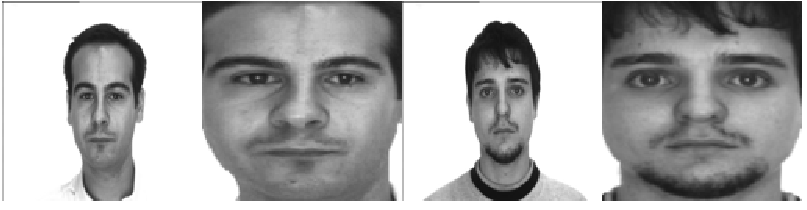
\includegraphics[scale=0.99]{imgs/violap.png}
\source{Jonas Mendonça Targino, 2018. Imagens de faces obtidas da base AR \cite{martinez1998ar}}
\label{fig:aplic_viola_jones}
\end{figure}

Após a fase de detecção da face, percebeu-se um baixo nível de oclusões (óculos de grau) na base Yale, podendo influenciar possíveis viés em termos de comparação. Mediante este problema, manipulou-se as 15 imagens presentes na base Yale com baixos níveis de oclusões e para cada imagem foram geradas duas outras, uma com oclusão de óculos e outra com oclusão de cachecol como forma de deixar os grupos comparáveis em termos de oclusões, obtendo-se assim 30 imagens parcialmente ocluídas. Um observação importante a respeito das máscaras de oclusões dessa base é que as mesmas foram obtidas por meio de recortes de imagens parcialmente ocluídas da base AR, podendo ser visualizada conforme a figura \ref{fig:mascaras}.


\begin{figure}[H]
\centering
\caption{Imagens da base de dados Yale e suas respectivas máscaras de oclusão adicionadas}
\label{fig:mascaras}
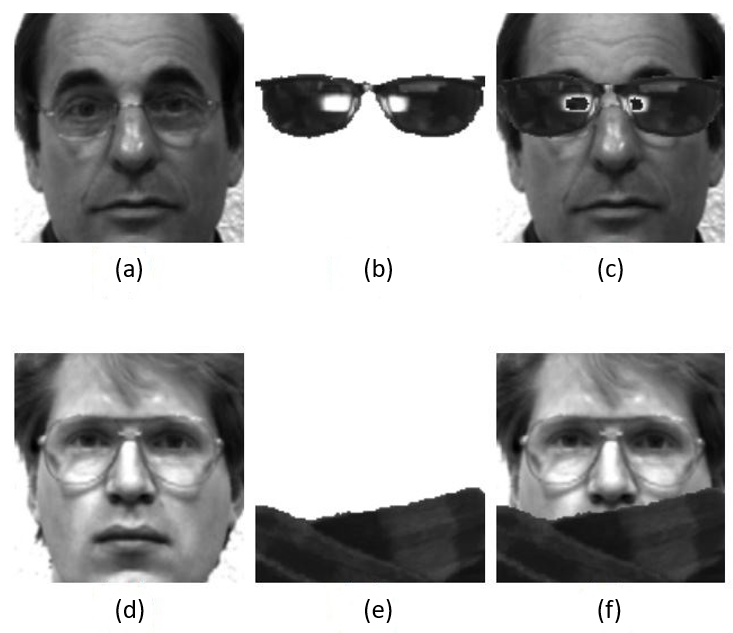
\includegraphics[scale=0.45]{imgs/pre_proce.png}
\begin{fignote} 
(a) e (d) imagens com baixo nível de oclusão; (b) e (e) máscaras de oclusão; (c) e (f) imagens geradas com consideráveis níveis de oclusão parcial  
\end{fignote}
\source{Jonas Mendonça Targino, 2018. As duas primeiras imagens foram obtidas da base Yale \cite{georghiades1997yale}}
\end{figure}

Para a extração de características foi aplicada a TW utilizando três níveis de decomposição com coeficientes de aproximação (LL) e as seguintes funções Wavelet: Daubechies 2, Daubechies 4, Symlet 3, Symlet 4 e Symlet 5. Na tabela \ref{tab:coefWav} são apresentadas as funções Wavelets bem como suas respectivas quantidades de características extraídas por cada coeficiente de aproximação.

\begin{table}[H]
\caption{Número de características extraídas com a transformada Wavelet de acordo com cada nível de decomposição}
\centering
\begin{tabular}{|c|c|c|c|}
\cline{2-4}
 \multicolumn{1}{c|}{} & \multicolumn{3}{c|}{\textbf{\#  características}}\\ \hline
\multicolumn{1}{|c|}{\multirow{1}{*}{\textbf{Função Wavelet} }}& \textbf{LL1} &  \textbf{LL2} &  \textbf{LL3}   \\\hline
Daubechies 2 & 4225 & 1156 & 324 \\\hline
Daubechies 4 & 4489 & 1369 & 484 \\\hline
Symlet 3 & 4356 & 1225 & 400 \\\hline
Symlet 4 & 4489 & 1369 & 484 \\\hline
Symlet 5 & 4624 & 1444 & 529 \\\hline
\end{tabular}
\source{Jonas Mendonça Targino, 2018}
\label{tab:coefWav}
\end{table}


Objetivando normalizar os dados foi aplicada a normalização pela média e desvio padrão conforme apresentada em \cite{galdi2016multimodal}, garantindo que cada coluna apresente média 0 e desvio padrão 1 como descrito conforme a equação \ref{eq:norm_std}, em que $x_j$, $\bar{x_j}$ e $\sigma_j$ significam respectivamente a coluna $x_j$, sua média e seu desvio padrão.

\begin{equation}
\label{eq:norm_std}
f(x_{j}) = \frac{(x_j - \bar{x_j})}{\sigma_j}  
\end{equation}


\section{Divisões dos experimentos} 


 
 De modo a separar cada tipo de oclusão e outras variações (iluminação) associadas à oclusão objetivando entender o comportamento das técnicas de reconstrução foi necessário dividir o conjunto conforme os tipos de oclusões e variações existentes.

Com as bases selecionadas, verificou-se de forma detalhada cada base de dados, de maneira a investigar tipos de oclusões presentes e tipos de variações existentes. Após identificada a oclusão selecionou-se as oclusões com cachecol e óculos de sol.

Mediante as duas bases de dados, percebeu-se que a base de dados AR apresentava algumas variações de oclusões, sendo elas: (\textit{i}) oclusões parciais de cachecol; (\textit{ii}) de óculos; (\textit{iii}) e de cachecol e óculos com variações de iluminação. Já base de dados Yale apresentava apenas oclusões de cachecol e óculos, as quais foram inseridas de maneira artificial utilizando a máscara de oclusão da base AR. 

A partir disso conseguiu-se dividir as bases de dados em 6 grupos, com siglas referentes a base e número do experimento. Essas siglas podem serem visualizadas a seguir:


\begin{enumerate}
\item \textbf{AR\#1}: contém todas as imagens parcialmente ocluídas presentes na base de dados AR, sendo no total 1200 imagens;
\item \textbf{AR\#2}: contém as imagens presentes na base AR com oclusão de óculos de sol e cachecol sem iluminação, sendo no total 400 imagens;
\item \textbf{AR\#3}: contém as imagens apenas com oclusão de óculos de sol sendo no total 600 imagens;
\item \textbf{AR\#4}: contém as imagens presentes na base AR que possuem oclusões parciais de cachecol sendo no total 600 imagens;
\item \textbf{Yale\#1}: compreende 15 imagens da base Yale com oclusões de óculos;
\item \textbf{Yale\#2}: compreende 15 imagens da base Yale com oclusões de cachecol. 
\end{enumerate}


\section{Resultados das bases de dados antes da reconstrução}


Antes de apresentar a acurácia de reconhecimento das técnicas baseadas em subespaço para a tarefa de reconstrução é interessante visualizar a acurácia de reconhecimento do classificador após aplicação da imagem pura com oclusão. Mediante isso os resultados abaixo apresentam o comportamento da taxa de reconhecimento das bases mediante avaliação com os classificadores ELM, KNN e SVM.


\subsection{Resumindo os resultados pré-reconstrução das imagens}

Ao analisarmos os grupos gerados é interessante analisarmos a acurácia dos grupos antes de reconstruir as faces parcialmente ocluídas, de modo a verificarmos a complexidade do conjunto. Na figura \ref{fig:acuracia_AR_ELM_KNN} podemos perceber a acurácia dos seis grupos gerados nas duas bases de dados com os classificadores KNN, ELM e SVM. Podendo visualizar que nos quatro grupos da base AR encontram-se imagens com altos níveis de oclusão, implicando em baixas taxas de reconhecimento das imagens parcialmente ocluídas. Enquanto os dois grupos da base Yale apresentaram apenas imagens ocluídas sem variações de iluminação conseguindo acurácia de 100\% nos grupos com classificador SVM. Desse modo todos os grupos foram analisados, porém os maiores focos nesse trabalho foram dados aos quatro grupos da base AR por lidarem com oclusões naturais.

\begin{figure}[H]
\centering
\caption{Acurácia dos grupos ocluídos com os classificadores KNN, ELM e SVM utilizando o nível 3 de decomposição da TW}
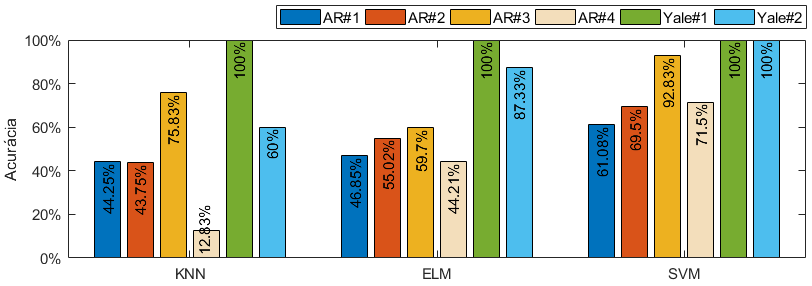
\includegraphics[scale=0.65]{imgs2/percentual_com_oclusao_AR_ELM}
\source{Jonas Mendonça Targino, 2018}
\label{fig:acuracia_AR_ELM_KNN}
\end{figure}


 
\section{Detecção da oclusão parcial na imagem de face}

Após a fase de segmentação da face, é interessante que  o sistema possa ser capaz de verificar se a imagem da face apresenta oclusão ou não. Essa etapa também chamada de DFFS  é responsável por projetar a face de entrada em um espaço de faces e a depender da distância existente entre aquela imagem e o espaço de faces a imagem é classificada como contendo oclusão ou não. A métrica DFFS apresenta-se eficiente quando almejamos descobrir se uma determinada face possui oclusão ou não. Logo essa métrica ao ser calculada obtém-se um valor, e caso esse valor seja superior ao limiar definido como 1.460 (valor definido com base em testes contendo imagens ocluídas e não ocluídas) a imagem apresenta oclusão na imagem da face, caso o valor do DFFS seja inferior ao limiar a imagem não apresenta oclusão na face. Podemos observar nas tabelas \ref{tab:valoresDFFS_AR} e \ref{tab:valoresDFFS_Yale} respectivamente o DFFS nas bases \textit{AR} e \textit{Yale}, apresentando a média e desvio padrão a depender da presença da oclusão ou não, na imagem da face. 


A partir da análise das tabelas \ref{tab:valoresDFFS_AR} e \ref{tab:valoresDFFS_Yale} podemos perceber que a base de dados \textit{AR} apresenta níveis maiores de oclusões quando comparada a base de dados \textit{Yale}. 


\begin{table}[H]
  \centering
  \caption{Valores de DFFS de acordo com a base de dados \textit{AR}}
    \begin{tabular}{c|c|c}
    %\toprule
    Tipo de imagem & \multicolumn{1}{l|}{Média DFFS} & \multicolumn{1}{l}{Desvio padrão} \\
    \midrule
    Sem oclusão & 908.79   & $\pm 138.13 $ \\
    \midrule
    Com oclusão & 2392.21 & $\pm 411.67 $ \\
    \bottomrule
    \end{tabular}%
  \label{tab:valoresDFFS_AR}%
   \source{Jonas Mendonça Targino, 2018}
\end{table}%




\begin{table}[H]
  \centering
  \caption{Valores de DFFS de acordo com a base de dados \textit{Yale}}
    \begin{tabular}{c|c|c}
    %\toprule
    Tipo de imagem & \multicolumn{1}{l|}{Média DFFS} & \multicolumn{1}{l}{Desvio padrão} \\
    \midrule
    Sem oclusão & 832,32   & $\pm 355,64$ \\
    \midrule
    Com oclusão & 2.550,46 & $ \pm 684,16$ \\
    \bottomrule
    \end{tabular}%
  \label{tab:valoresDFFS_Yale}%
   \source{Jonas Mendonça Targino, 2018}
\end{table}%



Neste trabalho foram utilizadas algumas técnicas para detecção da parte ocluída. Inicialmente foram realizados alguns testes com \textit{Skin Tone}, o qual apresentou sensibilidades no processo de segmentação quando apresentado a ambientes não controlados. Logo em seguida foi utilizada a técnica de limiarização, em que a mesma utiliza um limiar para segmentação da parte ocluída na imagem da face, com base em alguns testes foi definido o limiar 78 como delimitador de oclusões nas regiões de face. 

A partir do uso desse limiar como método base para detecção da oclusão, analisou-se a imagem pixel a pixel e todos os pixels com valores menores ou iguais ao limiar foram atribuídos valor zero (ou seja, na escala de cinza equivalente a cor preta). 


Essa técnica apresentou resultados de segmentação um pouco melhores que o Skin Tone, entretanto, ao se implementar a técnica  BMA foram visualizadas melhores performances de detecção da parte ocluída, por analisar todos os pixels da imagem por meio de uma máscara de dimensão (2 $\times$ 2), dessa forma fixando o BMA como técnica para detecção da oclusão para todas as técnicas. A figura \ref{fig:mascaraOclusao} ilustra algumas máscaras de oclusão obtidas com BMA.

\begin{figure}[H]
\caption{Máscaras de oclusões em algumas imagens da base de dados\textit{AR}}
\center
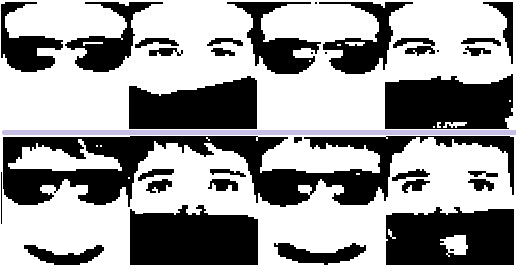
\includegraphics{imgs/mascaraOclusao.png}
\source{Jonas Mendonça Targino, 2018}
\label{fig:mascaraOclusao}
\end{figure}
 
Após a detecção da oclusão foram aplicados alguns operadores morfológicos com a finalidade de aplicar melhorias na máscara ocluída e com isso possibilitar uma detecção da oclusão de forma mais robusta. A partir dos operadores morfológicos utilizados, alguns se destacaram um pouco mais, dentre os que apresentaram melhorias na máscara estão: erosão, dilatação, abertura e fechamento. A aplicação desses filtros em uma imagem de face pode ser visualizada na figura \ref{fig:operadoresmorfologicos}, nesta figura podemos perceber a variação da imagem original perante a aplicação dos filtros morfológicos. Dentre os operadores morfológicos, o que apresentou melhores resultados foi o operador de erosão por questões do mesmo realçar mais detalhadamente a região ocluída na imagem da face. No entanto todos os outros três operadores também foram utilizados, com iniciativas a produzir melhores áreas de detecção da parte ocluída.


\begin{figure}[H]
\centering
\caption{Aplicação da máscara de oclusão em operadores morfológicos}
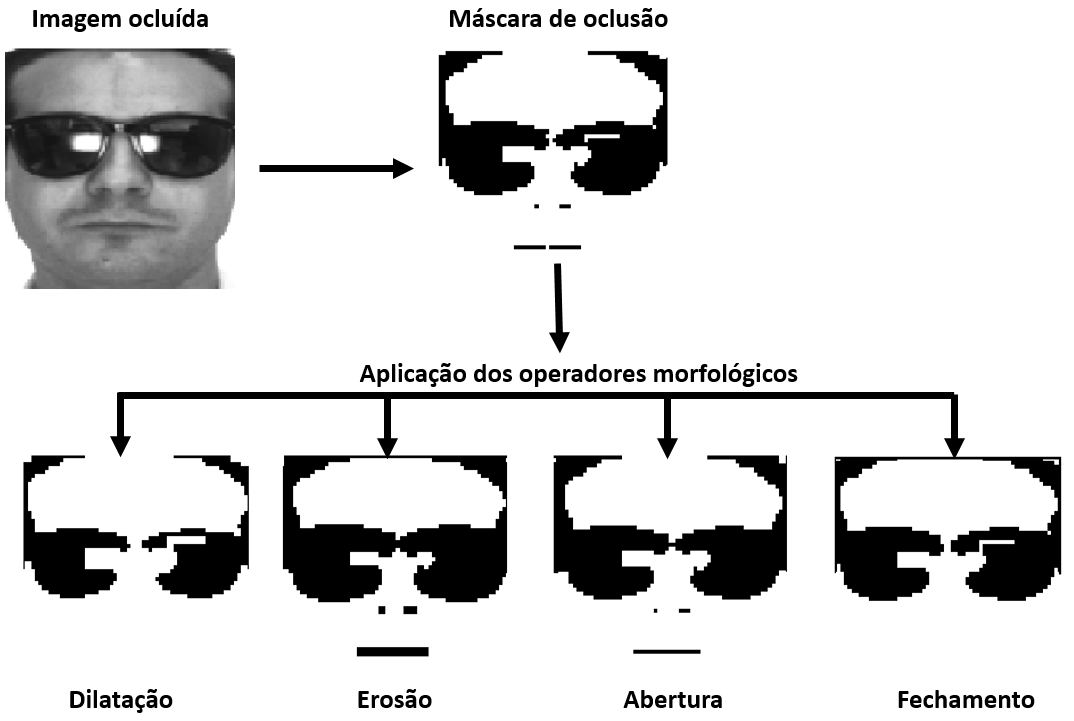
\includegraphics[scale = 0.5]{imgs3/mascara_oclusao}
\source{Jonas Mendonça Targino, 2018}
\label{fig:operadoresmorfologicos}
\end{figure}





\section{Resultados das técnicas baseadas em subespaço}

De modo a identificar todas as técnicas baseadas em subespaço foram criadas algumas abreviações para as técnicas de modo a realizar o posicionamento de maneira satisfatória frente a leitura do texto. Essas abreviações estão dispostas na tabela \ref{tab:tecnicas_subespaco}.

\begin{table}[htpb]
	\centering
	\caption{Abreviações geradas para algumas técnicas baseadas em subespaço}
    \label{tab:tecnicas_subespaco}
    %\space
	\begin{tabular}{|l|c|} \hline

		\textbf{Técnica}	& \textbf{Abreviação}  \\ \hline
		Base com oclusão  & BO  \\ \hline
		Asymmetrical PCA  & APCA  \\ \hline
		Fast Robust PCA & FRPCA \\ \hline
		Recursive PCA   &	 Rec PCA \\ \hline
		Fast Recursive PCA &	 Fast Rec PCA  \\ \hline
		Gappy PCA &	 GPCA  \\ \hline
		SRC Fast Recursive PCA & SRC Fast Rec PCA \\ \hline 
	\end{tabular}
\source{Jonas Mendonça Targino, 2018}
\end{table}

\subsection{Resultados nos grupos da base AR}

Com os experimentos realizados verificamos que as técnicas SRC Fast Rec PCA, Rec PCA e Fast Rec PCA apresentaram consideráveis resultados de reconstruções quando comparadas a outras técnicas baseadas em subespaço. Exemplos de oito imagens reconstruídas de dois indivíduos podem ser visualizadas com o auxílio da figura \ref{fig:exemplos_reconstrucoes}. Nessa figura é possível perceber o motivo dessas três técnicas apresentarem melhores resultados quando comparadas a outras técnicas, tal fato, se deve a essas técnicas minimizarem os coeficientes de combinação linear. Um grande diferencial das técnicas SRC Fast Rec PCA, Rec PCA e Fast Rec PCA é a substituição dos pixels não ocluídos pelos pixels da imagem original, de modo a evitar maiores inserções de ruídos na imagem reconstruída.

\begin{figure}[H]
\centering
\caption{Exemplos de imagens reconstruídas de dois indivíduos de acordo com os grupos da base AR}
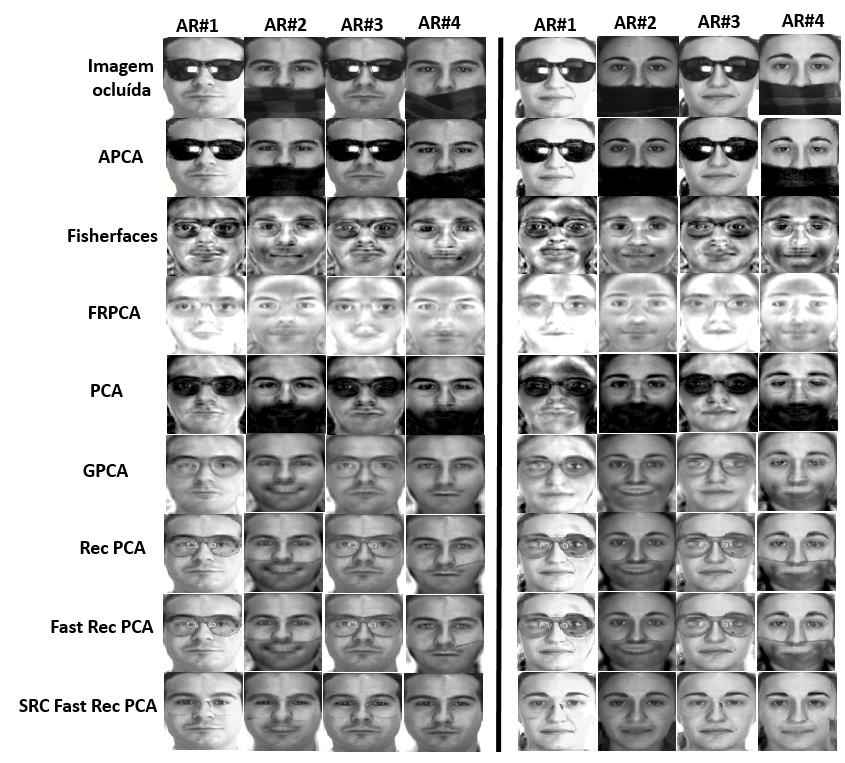
\includegraphics[scale=0.68]{imgs4/reconstrucoes_subespaco}
\source{Jonas Mendonça Targino, 2018}
\label{fig:exemplos_reconstrucoes}
\end{figure}




Após a realização dos experimentos com as técnicas baseadas em subespaço foi analisada a qualidade da imagem reconstruída. E para a análise da qualidade da mesma foram utilizadas as métricas RMSE, SSIM e PSNR. Na tabela \ref{tab:RMSE_subespaco} é possível visualizar os resultados em termos de RMSE das técnicas baseadas em subespaço. Nessa mesma tabela é possível perceber que a técnica SRC Fast Rec PCA apresentou melhores resultados de RMSE, seguida pela técnica GPCA, Fast Rec PCA e Rec PCA. Por último a técnica Fast Robust PCA foi a técnica que apresentou os piores resultados.


\begin{table}[H]
\caption{Resultados de RMSE das técnicas baseadas em subespaço nos quatro grupos da base AR}
\centering
\begin{tabular}{|c|c|c|c|c|}
\cline{2-5}
 \multicolumn{1}{c|}{} & \multicolumn{4}{c|}{\textbf{RMSE}}\\ \hline
\multicolumn{1}{|c|}{\multirow{2}{*}{\textbf{Técnica} }}& \textbf{AR\#1} &  \textbf{AR\#2} & \textbf{AR\#3} & \textbf{AR\#4 }  \\ \cline{2-5}

& média $\pm$ desvio & média $\pm$ desvio & média $\pm$ desvio & média $\pm$ desvio \\\hline 
APCA			&73.37$\pm$11.09 &	66.43$\pm$12.55  &69.67$\pm$10.02	&77.07$\pm$10.88 \\\hline
FRPCA			&94.58$\pm$13.48 &	82.37$\pm$9.42	 &98.18$\pm$12.34	&90.99$\pm$13.63 \\\hline
Fast Rec PCA	&54.59$\pm$13.86 &	38.08$\pm$8.46	 &52.98$\pm$14.48	&56.20$\pm$13.02 \\\hline
GPCA			&53.09$\pm$13.31 &	36.91$\pm$7.14	 &52.07$\pm$14.02	&54.10$\pm$12.50 \\\hline
PCA				&72.92$\pm$10.39 &	69.83$\pm$12.47  &70.07$\pm$10.01	&75.78$\pm$9.97 \\\hline
Rec PCA			&54.59$\pm$13.86 &	38.07$\pm$8.48	 &52.97$\pm$14.49	&56.20$\pm$13.02\\\hline
Fisherfaces		&58.76$\pm$7.61  &	53.53$\pm$6.35	 &61.57$\pm$6.80	&55.95$\pm$7.34\\\hline
SRC Fast PCA    &\textbf{49.09$\pm$18.84} &	\textbf{25.84$\pm$9.98}	 &\textbf{50.42$\pm$20.19}	&\textbf{47.76$\pm$17.30} \\\hline


\end{tabular}
\source{Jonas Mendonça Targino, 2018}
\label{tab:RMSE_subespaco}
\end{table}


Em valores de SSIM as técnicas SRC Fast Rec PCA, GPCA, Rec PCA e Fast Rec PCA nessa ordem apresentaram os melhores resultados para todos os quatro grupos da base AR. Enquanto a técnica Fast Robust PCA novamente apresentou os piores resultados. Esses resultados estão dispostos na tabela \ref{tab:ssim_subespaco}.


\begin{table}[H]
\caption{Resultados de SSIM das técnicas baseadas em subespaço nos quatro grupos da base AR}
\centering
\begin{tabular}{|c|c|c|c|c|}
\cline{2-5}
 \multicolumn{1}{c|}{} & \multicolumn{4}{c|}{\textbf{SSIM}}\\ \hline
\multicolumn{1}{|c|}{\multirow{2}{*}{\textbf{Técnica} }}& \textbf{AR\#1} &  \textbf{AR\#2} & \textbf{AR\#3} & \textbf{AR\#4}   \\ \cline{2-5}
& média $\pm$ desvio & média $\pm$ desvio & média $\pm$ desvio & média $\pm$ desvio \\\hline 
APCA			&0.42$\pm$0.06	&0.45$\pm$0.06	&0.45$\pm$0.05&	0.39$\pm$0.05\\\hline
FRPCA			&0.46$\pm$0.04	&0.50$\pm$0.04	&0.48$\pm$0.04&	0.45$\pm$0.05\\\hline
Fast Rec PCA	&0.52$\pm$0.07	&0.59$\pm$0.06	&0.54$\pm$0.06&	0.50$\pm$0.08\\\hline
GPCA			&0.55$\pm$0.07	&0.61$\pm$0.06	&0.56$\pm$0.06&	0.53$\pm$0.08\\\hline
PCA				&0.37$\pm$0.05	&0.39$\pm$0.05	&0.39$\pm$0.05&	0.36$\pm$0.05\\\hline
Rec PCA			&0.52$\pm$0.07	&0.59$\pm$0.06	&0.54$\pm$0.06&	0.50$\pm$0.08\\\hline
Fisherfaces		&0.36$\pm$0.06	&0.41$\pm$0.04	&0.34$\pm$0.05&	0.38$\pm$0.05\\\hline
SRC Fast PCA    &\textbf{0.63$\pm$0.10}	&\textbf{0.71$\pm$0.09}	&\textbf{0.65$\pm$0.08}&	\textbf{0.60$\pm$0.11}\\\hline
\end{tabular}
\source{Jonas Mendonça Targino, 2018}
\label{tab:ssim_subespaco}
\end{table}

Enquanto ao analisar-se as técnicas baseadas em subespaço sobre a métrica PSNR obteve-se a mesma conclusão das outras métricas. De modo que novamente as técnicas as quatro técnicas apresentaram os melhores resultados. E a técnica Fast Robust PCA novamente apresentou os piores resultados. Na tabela \ref{tab:psnr_subespaco} são apresentados tais resultados. 

\begin{table}[H]
\caption{Resultados de PSNR das técnicas baseadas em subespaço nos quatro grupos da base AR}
\centering
\begin{tabular}{|c|c|c|c|c|}
\cline{2-5}
 \multicolumn{1}{c|}{} & \multicolumn{4}{c|}{\textbf{PSNR}}\\ \hline
\multicolumn{1}{|c|}{\multirow{2}{*}{\textbf{Técnica} }}& \textbf{AR\#1} &  \textbf{AR\#2} & \textbf{AR\#3} &\textbf{ AR\#4}   \\ \cline{2-5}
& média $\pm$ desvio & média $\pm$ desvio & média $\pm$ desvio & média $\pm$ desvio \\\hline 
APCA			&10.56$\pm$1.42&	11.47$\pm$1.60&	11.00$\pm$1.46 &	10.12$\pm$1.23 \\\hline
FRPCA			&8.34$\pm$1.61 &	9.51$\pm$1.42 &	8.00$\pm$1.48  &	8.69$\pm$1.67 \\\hline
Fast Rec PCA	&13.35$\pm$2.62&	16.35$\pm$1.96&	13.67$\pm$2.84 &	13.04$\pm$2.34 \\\hline
GPCA			&13.59$\pm$2.62&	16.58$\pm$1.95&	13.81$\pm$2.85 &	13.37$\pm$2.36 \\\hline
PCA				&10.60$\pm$1.19&	11.03$\pm$1.42&	10.95$\pm$1.18 &	10.25$\pm$1.09 \\\hline
Rec PCA			&13.35$\pm$2.62&	16.36$\pm$1.96&	13.67$\pm$2.84 &	13.04$\pm$2.34 \\\hline
Fisherfaces		&12.46$\pm$1.46&	13.25$\pm$1.38&	12.03$\pm$1.33 &	12.88$\pm$1.47 \\\hline
SRC Fast PCA	&\textbf{14.83$\pm$4.31}&	\textbf{20.09$\pm$3.05}&	\textbf{14.70$\pm$4.57} &	\textbf{14.96$\pm$4.03} \\\hline
\end{tabular}
\source{Jonas Mendonça Targino, 2018}
\label{tab:psnr_subespaco}
\end{table}



Após análise de métricas de qualidade da imagem foi utilizada a taxa de acurácia de modo a tentar realizar justificativas complementares a essas métricas, com vista a analisar o desempenho de cada técnica perante a tarefa de reconstrução. 



O primeiro classificador a ser utilizado como forma de analisar a acurácia das técnicas foi o classificador KNN com nível 3 de decomposição da TW de modo que os melhores resultados foram provenientes da técnica SRC Fast Rec PCA, conseguindo 84.58\%, 92.50\%, 93.83\% e 75.33\% respectivamente nos grupos AR\#1, AR\#2, AR\#3 e AR\#4. Enquanto técnicas como o PCA, FRPCA e Fisherfaces apresentaram os piores resultados de acurácia. Ao passo que as técnicas Fast Rec PCA, Rec PCA e GPCA apresentaram acurácias próximas a 80\% apenas no grupo AR\#3. Todavia, no grupo AR\#4 todas as técnicas baseadas em subespaço com exceção da técnica SRC Fast Rec PCA apresentaram percentuais de identificação menor que 28\%. A figura \ref{fig:acuracia_KNN_AR_4_grupos} ilustra o comportamento das técnicas baseadas em subespaço com classificador KNN utilizando nível 3 de decomposição da TW.


\begin{figure}[H]
\centering
\caption{Acurácia com KNN com decomposição nível 3 da TW sobre os quatro grupos de oclusões presentes na base AR}
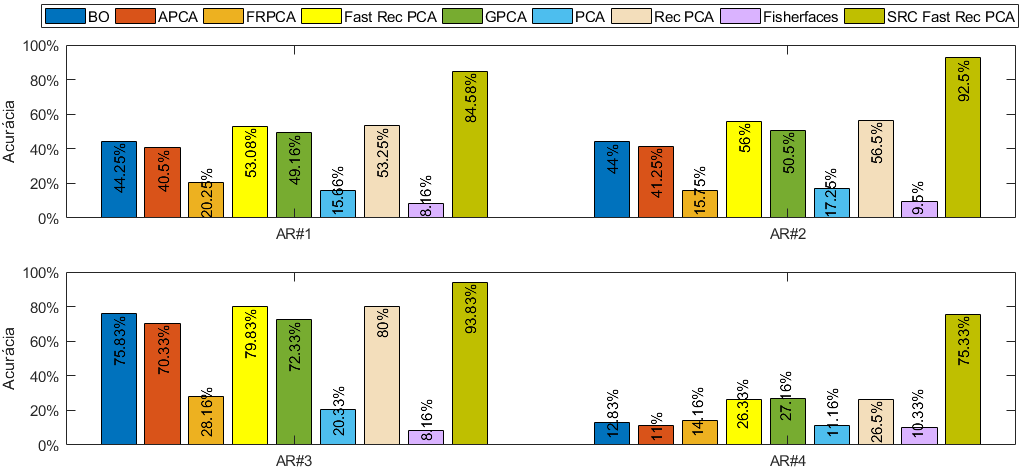
\includegraphics[scale=0.56]{imgs4/acuracia_subespaco_KNN}
\source{Jonas Mendonça Targino, 2018}
\label{fig:acuracia_KNN_AR_4_grupos}
\end{figure}

Ao realizarmos outro experimento com o classificador KNN utilizando nível 2 de decomposição da TW, obteve-se os resultados que são apresentados com o auxílio da figura \ref{fig:acuracia_KNN_AR_4_grupos_nivel2}. Nessa figura podemos perceber o comportamento das técnicas ao serem classificadas. Logo é possível perceber o maior grau de contribuição com a técnica SRC Fast Rec PCA apresentando 86\%, 93\%, 94.83\% e 77.33\% de acurácia nos grupos AR\#1, AR\#2, AR\#3 e AR\#4 respectivamente. Enquanto as técnicas Fast Rec PCA, Rec PCA e GPCA apresentaram resultados de acurácia um pouco mais próximos da técnica SRC Fast Rec PCA apenas no grupo AR\#3.

\begin{figure}[H]
\centering
\caption{Acurácia com KNN com decomposição nível 2 da TW sobre os quatro grupos de oclusões presentes na base AR}
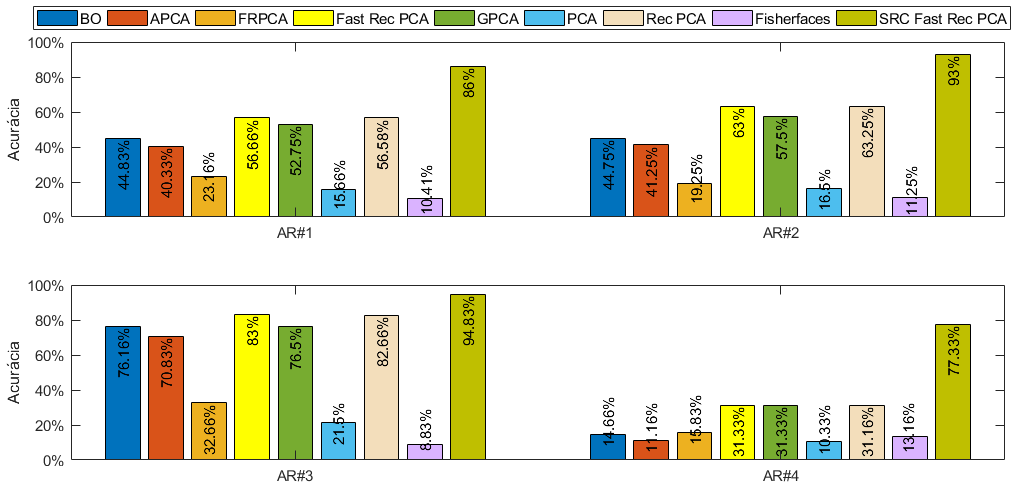
\includegraphics[scale=0.56]{imgs4/acuracia/nivel_one_two/KNNnivel2subespaco}
\source{Jonas Mendonça Targino, 2018}
\label{fig:acuracia_KNN_AR_4_grupos_nivel2}
\end{figure}

Paralelamente ao analisar o nível 1 da TW com classificador KNN a técnica SRC Fast Rec PCA novamente apresentou consideráveis percentuais de acurácia perante os quatro grupos da base AR, conforme ilustrado na figura \ref{fig:acuracia_KNN_AR_4_grupos_nivel1}. Em que podemos visualizar 13.25\%, 7\%, 4.84\% e 21.67\% de taxas de erro dessa técnica nos grupos AR\#1, AR\#2, AR\#3 e AR\#4 respectivamente. Enquanto as outras técnicas apresentaram desempenhos inferiores em todos os quatro grupos.

\begin{figure}[H]
\centering
\caption{Acurácia com KNN com decomposição nível 1 da TW sobre os quatro grupos de oclusões presentes na base AR}
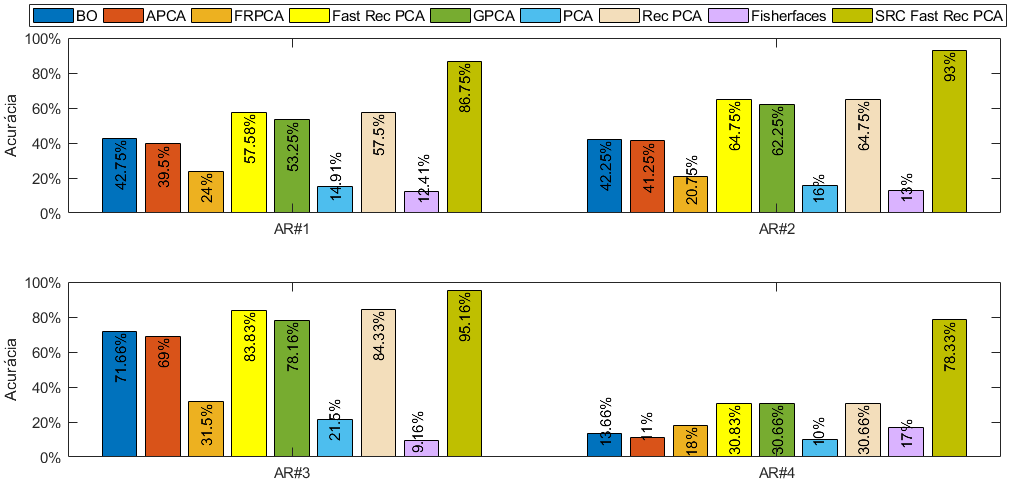
\includegraphics[scale=0.56]{imgs4/acuracia/nivel_one_two/knn_nivel1_subespaco}
\source{Jonas Mendonça Targino, 2018}
\label{fig:acuracia_KNN_AR_4_grupos_nivel1}
\end{figure}



Na figura \ref{fig:acuracia_ELM_AR_com_dois_contextos} é possível visualizar o desempenho de cada técnica baseada em subespaço perante a tarefa de reconstrução após análise dos resultados de acurácia com o classificador ELM utilizando nível 3 de decomposição da TW, por meio dessa figura podemos perceber  melhores percentuais de acurácia com a técnica SRC Fast Rec PCA, seguidamente das  técnicas Rec PCA, Fast Rec PCA e GPCA. De modo que a técnica SRC Fast Rec PCA alcançou percentuais de taxa de erro iguais a 10.67\%, 5.25\%, 3.67\% e 17\% nos grupos AR\#1, AR\#2, AR\#3 e AR\#4 respectivamente. Obtendo ganhos de reconstrução de 42.48\%, 39.55\%, 44.82\% e 38.79\%, nos grupos AR\#1, AR\#2, AR\#3 e AR\#4 na devida ordem.

\begin{figure}[H]
\centering
\caption{Acurácia das técnicas baseadas em subespaço com classificador ELM no nível 3 de decomposição da TW sobre os quatro grupos presentes na base AR}
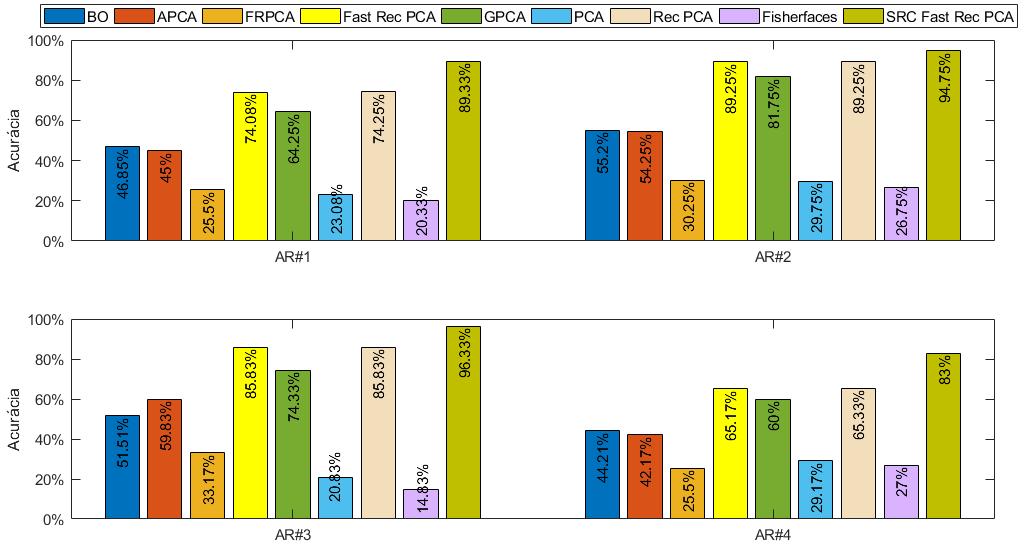
\includegraphics[scale=0.60]{imgs4/acuracia_subespaco_ELM}
\source{Jonas Mendonça Targino, 2018}
\label{fig:acuracia_ELM_AR_com_dois_contextos}
\end{figure}


Outro experimento similar foi aplicado utilizando o segundo nível de decomposição e classificador ELM, e novamente a técnica SRC Fast Rec PCA apresentou os melhores resultados em todos os quatro grupos da base AR. Conseguindo 90.17\%, 95.55\%, 96.17\% e 84.67\% de taxa de acurácia respectivamente nos grupos AR\#1, AR\#2, AR\#3 e AR\#4, conforme ilustra a figura \ref{fig:acuracia_ELM_AR_nivel2_subespaco}. Seguidamente as técnicas Rec PCA e Fast Rec PCA apresentaram resultados consideráveis nos grupos AR\#2 e AR\#3. 

\begin{figure}[H]
\centering
\caption{Acurácia das técnicas baseadas em subespaço com classificador ELM no nível 2 de decomposição da TW sobre os quatro grupos presentes na base AR}
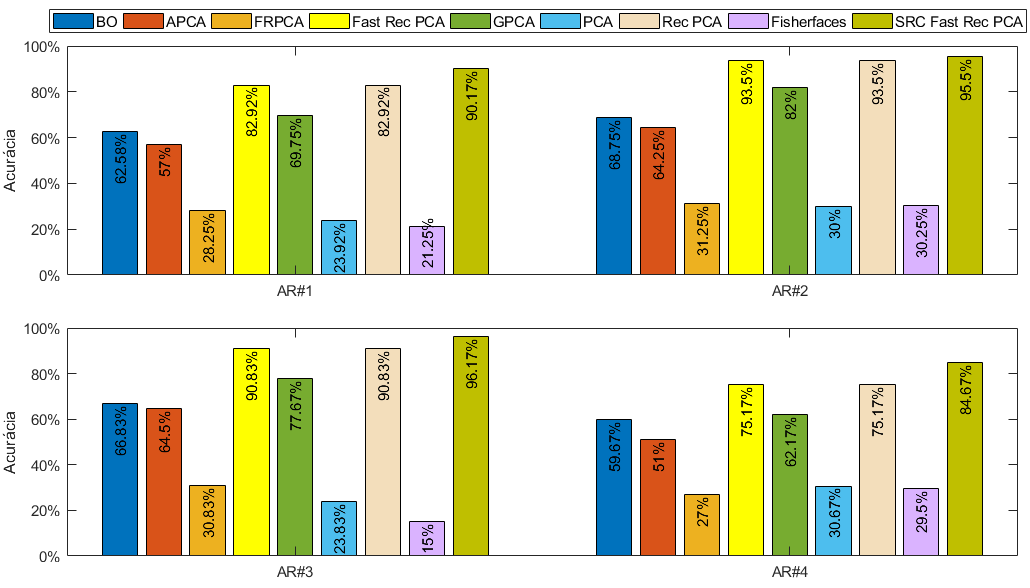
\includegraphics[scale=0.60]{imgs4/acuracia/nivel_one_two/ELM_nivel_2_subespaco}
\source{Jonas Mendonça Targino, 2018}
\label{fig:acuracia_ELM_AR_nivel2_subespaco}
\end{figure}


Enquanto na figura \ref{fig:acuracia_ELM_AR_nivel1_subespaco} podemos visualizar o comportamento das técnicas baseadas ao se utilizar o nível 1 de decomposição da TW com classificador ELM. Em que podemos visualizar que novamente a técnica SRC Fast Rec PCA apresentou os melhores resultados de acurácia, seguida pela técnica Rec PCA, Fast Rec PCA e GPCA. De modo que a técnica SRC Fast Rec PCA obteve taxas de erro iguais a 9.75\%, 5.5\%, 4.84\% e 15.5\%, assim como ganhos de reconstrução de 30\%, 30\%, 33.16\% e 24.84\% respectivamente nos grupos AR\#1, AR\#2, AR\#3 e AR\#4. 


\begin{figure}[H]
\centering
\caption{Acurácia das técnicas baseadas em subespaço com classificador ELM no nível 1 de decomposição da transformada Wavelet sobre os quatro grupos presentes na base AR}
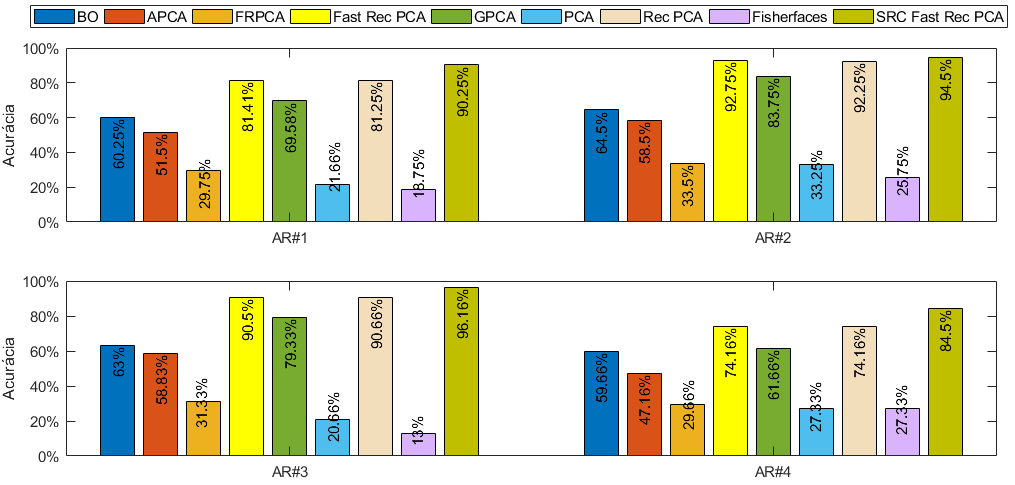
\includegraphics[scale=0.60]{imgs4/acuracia/nivel_one_two/ELM_nivel_1_subespaco}
\source{Jonas Mendonça Targino, 2018}
\label{fig:acuracia_ELM_AR_nivel1_subespaco}
\end{figure}


Ao avaliarmos as técnicas baseadas em subespaço com classificador SVM e nível 3 de decomposição os melhores resultados foram alcançados com as técnicas SRC Fast Rec PCA, obtendo taxas de erro iguais a 10.75\%, 5.75\%, 4.17\% e 16\% nos grupos AR\#1, AR\#2, AR\#3 e AR\#4 respectivamente. Enquanto as técnicas Rec PCA, Fast Rec PCA e GPCA apresentaram taxas de erros maiores que a apresentada pela técnica SRC Fast Rec PCA. Podemos visualizar com o auxílio da figura \ref{fig:acuracia_SVM_AR_4_grupos} o comportamento das técnicas com tais configurações.	

\begin{figure}[H]
\centering
\caption{Acurácia com SVM com nível 3 de decomposição da TW sobre os quatro grupos de oclusões presentes na base AR}
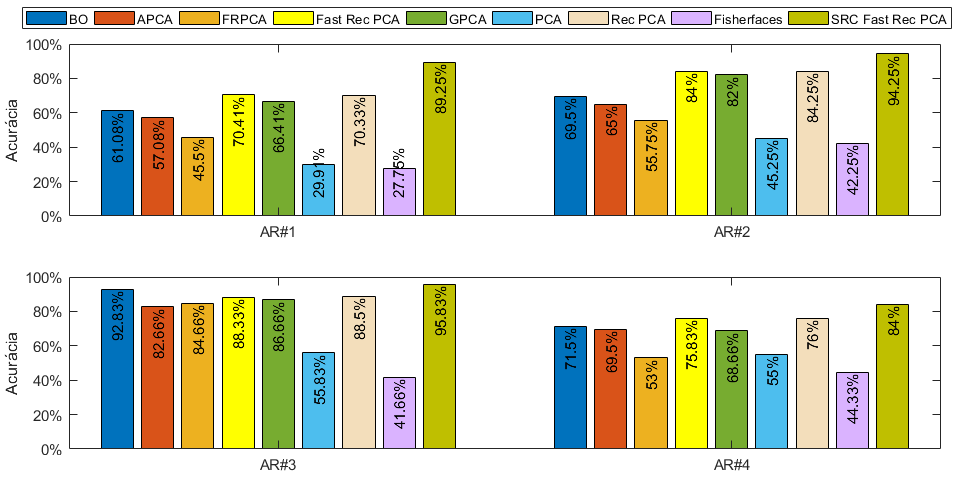
\includegraphics[scale=0.60]{imgs4/acuracia_subespaco_SVM}
\source{Jonas Mendonça Targino, 2018}
\label{fig:acuracia_SVM_AR_4_grupos}
\end{figure}

Paralelamente, ao se utilizar o nível 2 de decomposição da TW e classificador SVM podemos foi possível obter resultados ainda melhores para a técnica SRC Fast Rec PCA, a qual apresentou resultados superiores  de acurácia quando comparada as outras técnicas baseadas em subespaço, conforme ilustra a figura \ref{fig:acuracia_SVM_AR_4_grupos_nivel2}. Em que visualizamos taxas de erros iguais a 9.92\%, 5\%, 3.67\% e 14.84\% para os grupos AR\#1, AR\#2, AR\#3 e AR\#4 respectivamente. É válido mencionar o comportamento do classificador SVM ao lidar com pequenas oclusões parciais como oclusão de óculos, de modo que o SVM apresenta melhores resultados de acurácia na base com tais tipos de oclusões do que outros classificadores como KNN e ELM. Na figura \ref{fig:acuracia_SVM_AR_4_grupos_nivel2} podemos perceber tal afirmação no grupo AR\#3, em que a base ocluída (BO) apresentou 93.50\% de taxa acurácia.

\begin{figure}[H]
\centering
\caption{Acurácia com SVM com nível 2 de decomposição da TW sobre os quatro grupos de oclusões presentes na base AR}
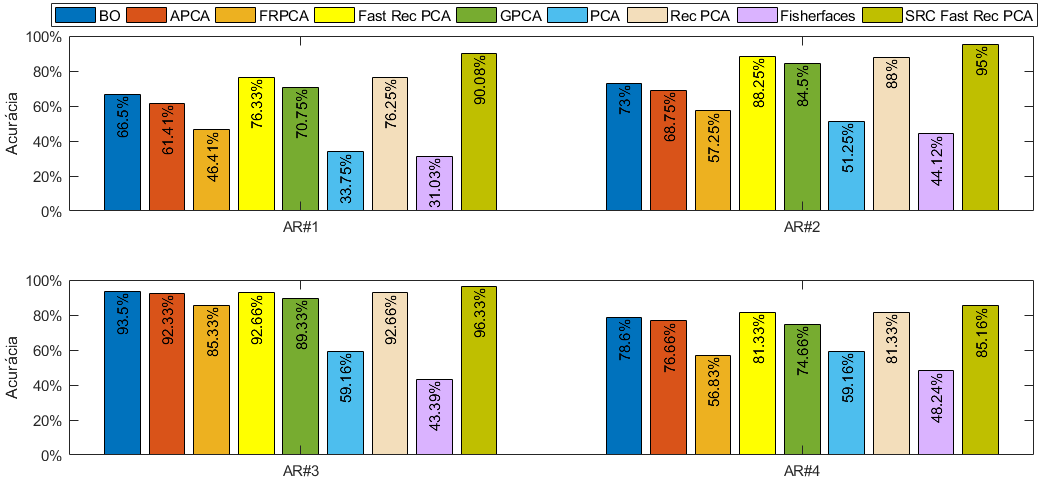
\includegraphics[scale=0.55]{imgs4/acuracia/nivel_one_two/SVM_nivel2_subespaco}
\source{Jonas Mendonça Targino, 2018}
\label{fig:acuracia_SVM_AR_4_grupos_nivel2}
\end{figure}



%\begin{figure}[H]
%\centering
%\caption{Acurácia com SVM com nível 1 de decomposição da TW sobre os quatro grupos de oclusões presentes na base AR}
%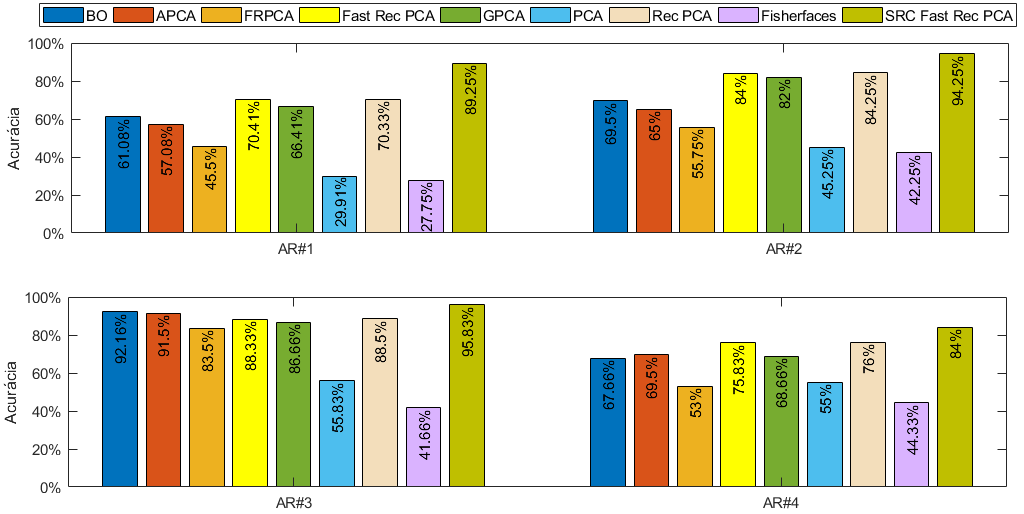
\includegraphics[scale=0.55]{imgs4/acuracia/nivel_one_two/SVM_nivel1_subespaco}
%\source{Jonas Mendonça Targino, 2018}
%\label{fig:acuracia_SVM_AR_4_grupos_nivel1}
%\end{figure}



Nesse trabalho ao utilizar outros níveis de decomposição com a TW verificou-se ganhos em algumas técnicas, e analisar os ganhos por níveis é interessante de modo a verificar a influência de cada nível para o reconhecimento da técnica. Dessa forma a seguir são apresentados os ganhos de cada técnica. Para apresentar esses ganhos foram criadas algumas siglas para diferenciá-las perante as demais. Logo a sigla BO representa a base ocluída, e as siglas T1 a T8 representam respectivamente as técnicas APCA, FRPCA, Fast Rec PCA, Rec PCA, GPCA, PCA, Fisherfaces e SRC Fast Rec PCA. 


Ao verificar os ganhos por nível com classificador KNN pode-se perceber com o auxílio da figura \ref{fig:ganhos_com_KNN_subespaco_AR} ganhos próximos entre o nível 1 e 2. Dessa forma, inferindo-se que o nível 1 não influenciou de forma significativa a acurácia de classificação. Garantindo-se resultados próximos de acurácia com base na melhor técnica de reconstrução, sendo ela o SRC Fast Rec PCA.

\begin{figure}[H]
\centering
\caption{Ganhos das técnicas baseadas em subespaço ao utilizar outros níveis de decomposição da TW com classificador KNN}
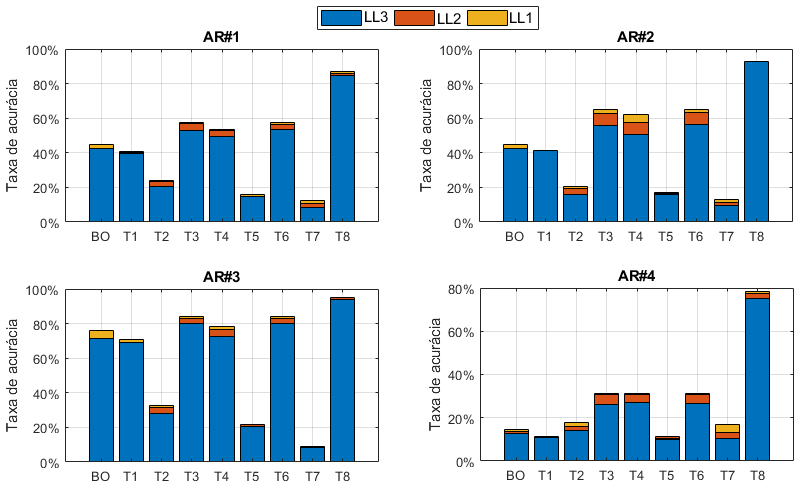
\includegraphics[scale=0.60]{imgs4/ganhos/ganhos_subespaco_KNN_niveis}
\source{Jonas Mendonça Targino, 2018}
\label{fig:ganhos_com_KNN_subespaco_AR}
\end{figure}



Tomando por base a figura \ref{fig:ganhos_com_ELM_subespaco_AR} é possível perceber melhorias de acurácia ao utilizar a base ocluída. De modo que paralelamente as técnicas GPCA, Fast Rec PCA e Rec PCA também apresentaram comportamentos similares. Também é possível inferir que a técnica SRC Fast Rec PCA apresentou resultados próximos de acurácia ao utilizar os três níveis de decomposição, dessa forma, não usufruindo de melhores resultados em sua acurácia.


\begin{figure}[H]
\centering
\caption{Ganhos das técnicas baseadas em subespaço ao utilizar outros níveis de decomposição da TW com classificador ELM}
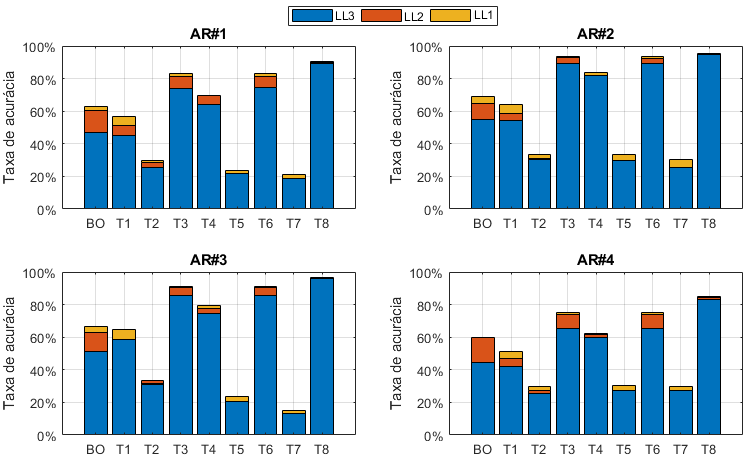
\includegraphics[scale=0.60]{imgs4/ganhos/ganhos_subespaco_ELM_niveis}
\source{Jonas Mendonça Targino, 2018}
\label{fig:ganhos_com_ELM_subespaco_AR}
\end{figure}




Um comportamento interessante das técnicas baseadas em subespaço ao utilizar outros níveis de decomposição com classificador SVM pode ser verificado com o auxílio da figura \ref{fig:ganhos_com_SVM_subespaco_AR}. Podendo perceber ganhos consideráveis ao utilizar o nível 2 de decomposição da Transformada Wavelet. De modo que todas as técnicas baseadas em subespaço, como também a base ocluída conseguiram melhores percentuais de reconhecimento.
\begin{figure}[H]
\centering
\caption{Ganhos das técnicas baseadas em subespaço ao utilizar os outros níveis de decomposição da TW com classificador SVM}
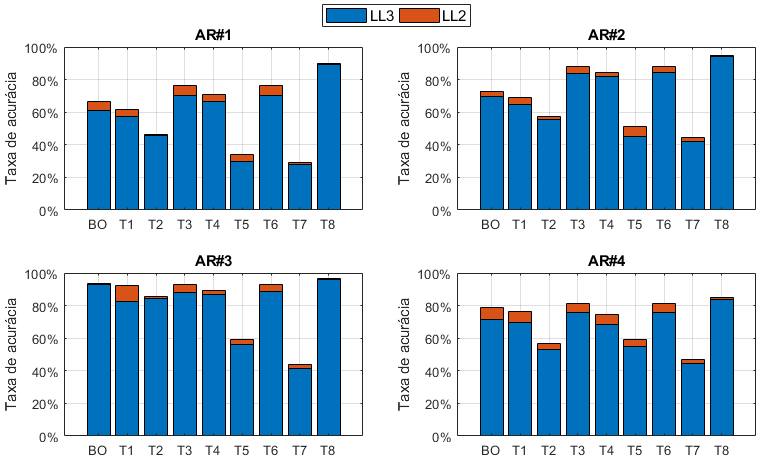
\includegraphics[scale=0.60]{imgs4/ganhos/ganhos_subespaco_SVM_niveis}
\source{Jonas Mendonça Targino, 2018}
\label{fig:ganhos_com_SVM_subespaco_AR}
\end{figure}


Ao demonstrar os resultados das técnicas em termos de acurácia e métricas de qualidade da imagem torna-se interessante também analisar o comportamento das técnicas em termos estatísticos. Dessa forma foi aplicado o teste estatístico de Wilcoxon \cite{litchfield1949simplified} sobre as técnicas. Esse teste é um método não paramétrico para análise de resultados de duas amostras pareadas, de forma que são calculados os valores numéricos da diferença entre cada par. De modo que foi analisada a amostra da melhor técnica baseada em subespaço com as outras técnicas, de forma que essas amostras foram obtidas por meio das 10 execuções da ELM para cada técnica. Os resultados estão dispostos na tabela \ref{tab:teste_estatistico_subespaco}. 

A hipótese nula em cada um dos testes são de que as amostras de cada técnica são oriundas da mesma distribuição com nível significância ($\alpha$) igual a $0.05$. Um valor $p$ maior que $\alpha$  significa que não podemos rejeitar a hipótese nula. Enquanto um valor $p$ menor que $\alpha$ significa que a hipótese nula foi rejeitada, concluindo que as duas técnicas comparadas são extraídas de duas distribuições significativamente diferentes. O \textit{p valor} de todas as comparações também estão incluídas na tabela \ref{tab:teste_estatistico_subespaco}. Logo foi possível concluir que a técnica SRC Fast Rec PCA apresentou os melhores resultados perante os quatro grupos de oclusões presentes na base AR.


\begin{table}[H]
    \centering
	\caption{Teste estatístico de Wilcoxon das técnicas baseadas em subespaço nos quatro grupos da base AR}
\begin{tabular}{|c|l|l|l|l|l|l|l|l|l|}
\hline
 &  & \multicolumn{8}{c|}{\textbf{Grupos}}  \\\cline{2-10}
 &  \multirow{2}{*}{\textbf{técnica}} & \multicolumn{2}{ c| }{\textbf{AR\#1}}
& \multicolumn{2}{ c| }{\textbf{AR\#2}}
& \multicolumn{2}{ c| }{\textbf{AR\#3}}
& \multicolumn{2}{ c| }{\textbf{AR\#4}}
\\\cline{3-10}
&  &  p valor & HN &  p valor & HN & p valor & HN  & p valor & HN
\\\hline
\multirow{7}{*}{\rotatebox[origin=c]{90}{\textbf{{\scriptsize	SRC Fast Rec PCA}}}}&
APCA			&0.0000&R		&0.0000&R	&0.0000&R		&0.0000&R  \\\cline{2-10}
&FRPCA			&0.0000&R		&0.0000&R	&0.0000&R		&0.0000&R  \\\cline{2-10}
& Fast Rec PCA	&0.0000&R		&0.0000&R	&0.0000&R		&0.0000&R  \\\cline{2-10}
& Rec PCA		&0.0000&R		&0.0000&R	&0.0000&R		&0.0000&R  \\\cline{2-10}
& GPCA			&0.0000&R		&0.0000&R	&0.0000&R		&0.0000&R  \\\cline{2-10}
& PCA			&0.0000&R		&0.0000&R	&0.0000&R		&0.0000&R  \\\cline{2-10}
& Fisherfaces	&0.0000&R		&0.0000&R	&0.0000&R		&0.0000&R  \\\hline
\end{tabular}

\begin{tablenotes}
		\centering
      	\footnotesize
      	\item HN = Hipótese Nula $\mid$ R = Rejeitada $\mid$ NR = Não Rejeitada
 
\end{tablenotes}
\source{Jonas Mendonça Targino, 2018}
\label{tab:teste_estatistico_subespaco}
\end{table}





Mediante análise das técnicas apresentadas acima percebeu-se resultados muito próximos de acurácia entre as técnicas Recursive PCA e Fast Recursive PCA. Logo, buscando analisar o erro por classe dessas técnicas na figura \ref{fig:taxa_erro_REC_PCA} é apresentado o erro por classe da técnica Recursive PCA. Sendo possível perceber que a maior incidência de erro por classe dessa técnica aconteceram nos grupos AR\#1 e AR\#4, estes grupos apresentam respectivamente imagens ocluídas com variações de iluminação e imagens com oclusão parcial de cachecol. 

Tais erros são justificados devido as imagens ocluídas possuírem poucos pixels não ocluídos e isso atrelado a variações de iluminações possibilitam maior distanciamento do espaço de faces, dessa forma, favorecendo que a combinação linear dos \textit{eigenfaces} produza uma imagem com maiores ruídos. Logo, os grupos que apresentaram menor taxa de erro foram os grupos AR\#2 e AR\#3, de modo que oclusões de óculos são um pouco menores que oclusões de cachecol, e paralelamente a ausência de iluminação na imagem favorece a reconstrução da imagem.

\begin{figure}[H]
\centering
\caption{Distribuição das taxas de erro geradas pela técnica Recursive PCA com o classificador ELM com nível 3 de decomposição da TW}
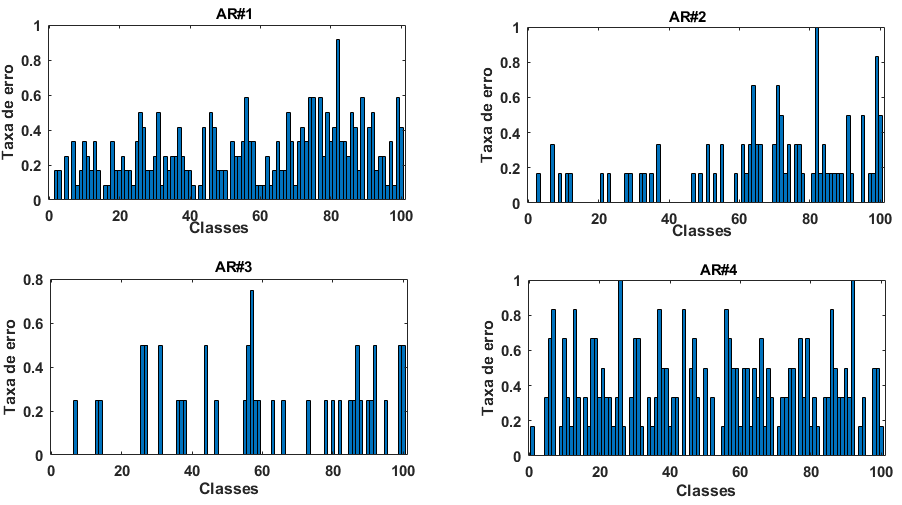
\includegraphics[scale=0.50]{imgs3/taxa_erro_REC_PCA.png}
\source{Jonas Mendonça Targino, 2018}
\label{fig:taxa_erro_REC_PCA}
\end{figure}

Também foram analisadas as taxas de erro com a técnica Gappy PCA, os mesmos encontram-se dispostos na figura \ref{fig:taxa_erro_GPCA}. Sendo possível perceber maiores taxas de erros nos grupos AR\#1 e AR\#4, enquanto que no grupo AR\#2 como o mesmo apresenta oclusões sem variações de iluminação a técnica Gappy PCA apresentou menor taxa de erros por classe quando comparado com os outros grupos.  

\begin{figure}[H]
\centering
\caption{Distribuição das taxas de erro geradas pela técnica Gappy PCA com o classificador ELM com nível 3 de decomposição da TW}
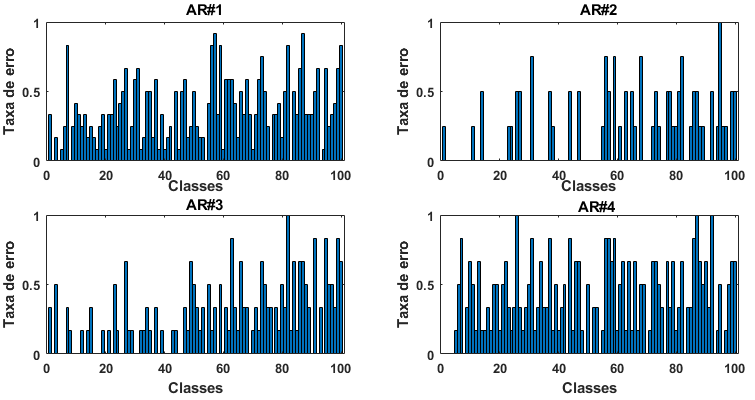
\includegraphics[scale=0.60]{imgs4/erro_GPCA_AR}
\source{Jonas Mendonça Targino, 2018}
\label{fig:taxa_erro_GPCA}
\end{figure}


Ao se analisar a taxa de erro por classe das técnicas baseadas em subespaço a técnica SRC com Fast Rec PCA   apresentou os melhores resultados. Na figura \ref{fig:taxa_erro_SRC_Fast_rec_PCA} são apresentados os gráficos de erro por classe em cada grupo da base AR. Sendo possível perceber maiores erros por classe no grupo AR\#4. Garantindo baixos percentuais de erro nos grupos AR\#2 e AR\#3.


\begin{figure}[H]
\centering
\caption{Distribuição das taxas de erro geradas pela técnica SRC com Fast Recursive PCA após análise com classificador ELM com nível 3 de decomposição da TW}
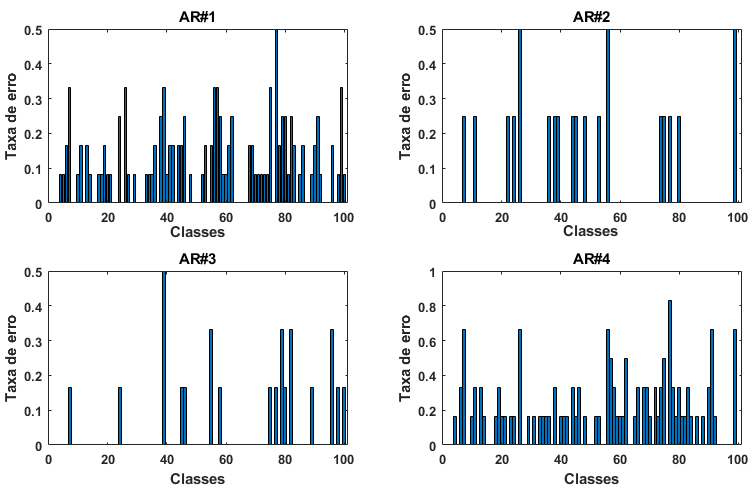
\includegraphics[scale=0.60]{imgs4/erro_por_classe_SRC_Fast_rec_PCA}
\source{Jonas Mendonça Targino, 2018}
\label{fig:taxa_erro_SRC_Fast_rec_PCA}
\end{figure}




Uma alternativa interessante ao analisar cada técnica é verificar quais classes de indivíduos apresentaram maiores taxas de erros e com quais outras classes foram confundidas. Dessa forma foram analisadas em termos de erro por classe das técnicas Recursive PCA, Gappy PCA e SRC Fast Rec PCA. Mediante tal propósito a figura \ref{fig:classes_erradas_FastRecPCA} ilustra em cada grupo da base AR quais classes obtiveram maior taxa de erro e ao lado a classe a qual foi confundida. Por exemplo, na figura \ref{fig:classes_erradas_FastRecPCA} no grupo AR\#1 a classe 82 apresentou o maior erro de reconhecimento, e na maioria desses erros a mesma foi confundida com a classe 72, levando em consideração a técnica de subespaço Recursive PCA.  Com isso, podemos perceber que as classes 82, 57, 82 e 26 apresentaram maiores erros para os grupos AR\#1, AR\#2, AR\#3 e AR\#4 respectivamente. De modo que tais classes foram confundidas com as classes 72, 48, 17 e 23 na devida ordem.


\begin{figure}[H]
\centering
\caption{Classes que apresentaram maior erro para cada grupo da base AR, como também os indivíduos confundidos após classificação com ELM para a técnica Recursive PCA}
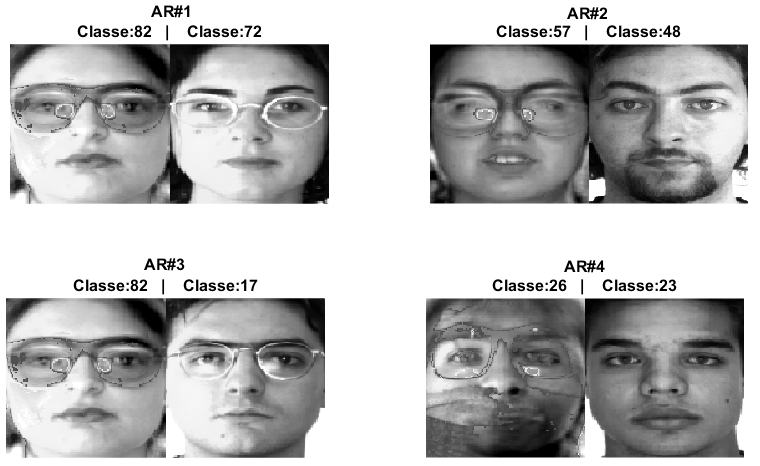
\includegraphics[scale=0.55]{imgs4/classes_erradas_FastRecPCA}
\source{Jonas Mendonça Targino, 2018}
\label{fig:classes_erradas_FastRecPCA}
\end{figure}

Paralelamente foram analisados os erros por classe da técnica Fast Recursive PCA, entretanto o mesmo apresentou resultados similares ao Recursive PCA, mediante isso, aqui são apresentados os erros por classe apenas da técnica Recursive PCA. 

Na figura \ref{fig:classes_erradas_GPCA} são apresentadas as classes que apresentaram maiores taxas de erro, bem como a classe em que o classificador classificou erroneamente para a técnica de reconstrução Gappy PCA. Em que podemos perceber que as classes 57, 95, 82 e 26 apresentaram maiores erros para os grupos AR\#1, AR\#2, AR\#3 e AR\#4 respectivamente. De modo que tais classes foram confundidas com as classes 5, 29, 19 e 42 na devida ordem.


\begin{figure}[H]
\centering
\caption{Classes que apresentaram maior erro para cada grupo da base AR, como também os indivíduos confundidos após classificação com ELM para a técnica Gappy PCA}
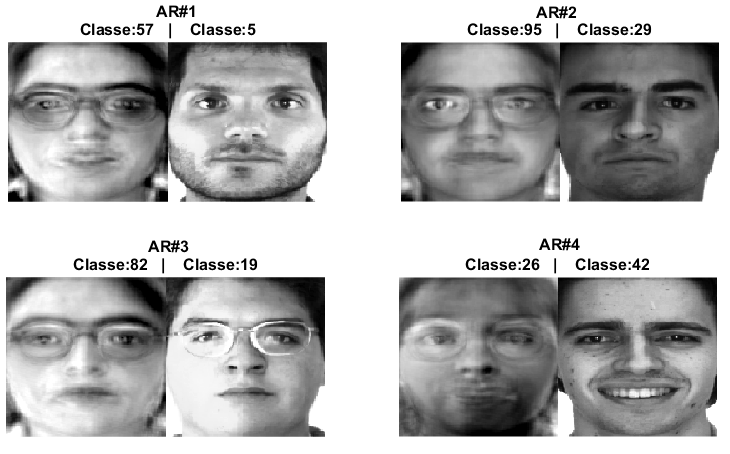
\includegraphics[scale=0.55]{imgs4/classes_erradas_GPCA}
\source{Jonas Mendonça Targino, 2018}
\label{fig:classes_erradas_GPCA}
\end{figure}

Enquanto a técnica SRC Fast Rec PCA apresentou maiores erros por classe nos grupos AR\#1, AR\#2, AR\#3 e AR\#4 respectivamente para as classes 77, 26, 39 e 77 as confundido com as classes 94, 74, 3 e 94 respectivamente. Na figura \ref{fig:classes_erradas_src_fast_rec_pca} são apresentadas as classes com maiores erros por grupo, assim como também as classes que foram confundidas.

\begin{figure}[H]
\centering
\caption{Classes que apresentaram maior erro para cada grupo da base AR, como também os indivíduos confundidos após classificação com ELM para a técnica SRC Fast Rec PCA}
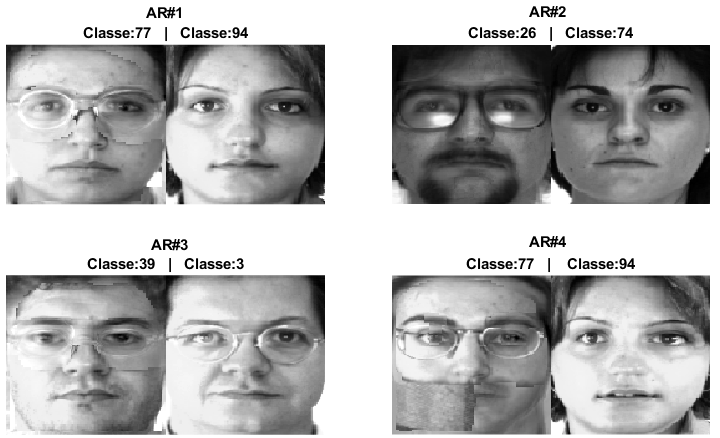
\includegraphics[scale=0.55]{imgs4/classes_confudidas_src_recPca}
\label{fig:classes_erradas_src_fast_rec_pca}
\source{Jonas Mendonça Targino, 2018}
\end{figure}



Com iniciativas a mensurar o desempenho das técnicas em termos de acurácia, precisão, F1-Score e MCC foram realizados os devidos experimentos para as três melhores técnicas baseadas em subespaço. Na tabela \ref{tab:teste_estatistico_fast_rec_pca} são apresentadas essas métricas de acordo com cada grupo da base AR, a partir das imagens reconstruídas com a técnica Fast Recursive PCA.



\begin{table}[htpb]
    \centering
    % \footnotesize
	\caption{Métricas de desempenho da técnica Fast Recursive PCA nos quatro grupos da base AR com classificador ELM e nível 3 de decomposição da TW}
\begin{tabular}{|c|c|c|c|c|}
\hline
\textbf{Grupos} & \textbf{Acurácia}  & \textbf{Precisão} & \textbf{F1-Score} & \textbf{MCC} \\\hline

AR\#1 &	0.7408	& 0.8113	& 0.7517	& 0.9236 \\\hline
AR\#2 &	0.8925	& 0.9280	& 0.8926	& 0.9003\\\hline
AR\#3 &	0.8567	&0.8927		& 0.8569	& 0.8642\\\hline
AR\#4 &	0.6500	&0.8483		& 0.6702	& 0.7126 \\\hline

\end{tabular}
\source{Jonas Mendonça Targino, 2018}
\label{tab:teste_estatistico_fast_rec_pca}
\end{table}

De forma paralela, na tabela \ref{tab:teste_estatistico_gappy_pca} são apresentados os valores das métricas a partir da técnica de reconstrução Gappy PCA. Pode-se perceber uma queda de performance para todas as métricas quando comparada com a técnica Fast Recursive PCA.

\begin{table}[htpb]
    \centering
    % \footnotesize
	\caption{Métricas de desempenho da técnica Gappy PCA nos quatro grupos da base AR com classificador ELM e nível 3 de decomposição da TW}
\begin{tabular}{|c|c|c|c|c|}
\hline
\textbf{Grupos} & \textbf{Acurácia} & \textbf{Precisão} & \textbf{F1-Score} & \textbf{MCC} \\\hline
AR\#1&	0.6425		&0.8170	& 0.6707	&0.6947 \\\hline
AR\#2&	0.8150		&0.8939	& 0.8217	& 0.8334 \\\hline
AR\#3&	0.7450		&0.8490	& 0.7514	&0.7703 \\\hline
AR\#4&	0.5983		&0.8356	& 0.6502	&0.6733 \\\hline
\end{tabular}
\source{Jonas Mendonça Targino, 2018}
\label{tab:teste_estatistico_gappy_pca}
\end{table}

Apresentando resultados muito próximos a técnica Fast Recursive PCA, a técnica Recursive PCA também demonstrou proximidades nas métricas de desempenho, apresentando valores das métricas bem próximos. Tais resultados estão dispostos na tabela \ref{tab:teste_estatistico_recursive_pca}.

\begin{table}[htpb]
    \centering
    %\footnotesize
	\caption{Métricas de desempenho da técnica Recursive PCA nos quatro grupos da base AR}
\begin{tabular}{|c|c|c|c|c|}
\hline
\textbf{Grupos} & \textbf{Acurácia} & \textbf{Precisão} & \textbf{F1-Score} & \textbf{MCC} \\\hline
AR\#1 &	0.7425	 &	0.8183	& 0.7537	& 0.7631 \\\hline
AR\#2 &	0.8925	 &	0.9285	& 0.8926 	& 0.9004 \\\hline
AR\#3 &	0.8583 	 &	0.8977	& 0.8599	& 0.8662 \\\hline
AR\#4 &	0.6533	 &	0.8475	& 0.6971	& 0.7153 \\\hline
 \end{tabular}
 \source{Jonas Mendonça Targino, 2018}
\label{tab:teste_estatistico_recursive_pca}
\end{table}


Enquanto ao verificarmos as métricas de desempenho com a técnica SRC Fast Rec PCA podemos perceber os melhores resultados dentre todas as outras técnicas baseadas em subespaço. Apresentando percentuais superiores de todas as métricas quando comparada as outras técnicas baseadas em subespaço. Sobressaindo-se com consideráveis percentuais perante os quatro grupos da base AR, de modo especial com melhores resultados nos grupos AR\#3, AR\#2 e AR\#1. Atuando como uma boa técnica que pode ser associada aos mais variados tipos de ambiente.


\begin{table}[htpb]
    \centering
	\caption{Métricas de desempenho da técnica SRC Fast Rec PCA nos quatro grupos da base AR}
\begin{tabular}{|c|c|c|c|c|}
\hline
\textbf{Grupos} & \textbf{Acurácia} & \textbf{Precisão} & \textbf{F1-score} & \textbf{MCC} \\\hline
AR\#1	&0.8983	&0.9132	&0.8948&	0.8980\\\hline
AR\#2	&0.9475	&0.9578	&0.9458&	0.9487\\\hline
AR\#3	&0.9633	&0.9695	&0.9623&	0.9640\\\hline
AR\#4	&0.8300	&0.8816	&0.8286&	0.8400\\\hline
\end{tabular}
\source{Jonas Mendonça Targino, 2018}
\label{tab:metricas_src_fast_rec_pca}
\end{table}










Tomando por base os resultados em termos de acurácia das técnicas baseadas em subespaço aplicadas no contexto biométrico, percebeu-se a viabilidade de analisar as taxas de FAR e FRR.
Na figura \ref{fig:FAR_FRR_APCA} são apresentadas as taxas de FAR e FRR da técnica Asymmetrical PCA para os quatros grupos da base AR. Para os limiares de semelhança iguais a 0.42, 0.54, 0.38 e 0.45 nos grupos AR\#1, AR\#2, AR\#3 e AR\#4 respectivamente as taxas de FAR e FRR apresentam valores iguais. De modo que, ambas as taxas apresentam valores próximos de 0.40, 0.33, 0.41 e 0.42. Logo, para cada grupo ao utilizarmos um limiar de semelhança menor que os valores de intersecção das respectivas curvas de FAR e FRR (no caso 0.42, 0.54,0.38 e 0.45) teremos a taxa de falsa maior, e isso implica em aceitar uma maior quantidade de pessoas que não estão cadastradas no sistema, as quais o sistema deveria rejeitar. Por outro lado, ao utilizar limiares de semelhança maiores de que o ponto de intersecção (EER), estaremos rejeitando uma maior quantidade de indivíduos que deveriam ser aceitos pelo sistema.   


\begin{figure}[H]
\centering
\caption{Curva com a taxa de falsa aceitação versus taxa de falsa rejeição alcançada pela técnica Asymmetrical PCA}
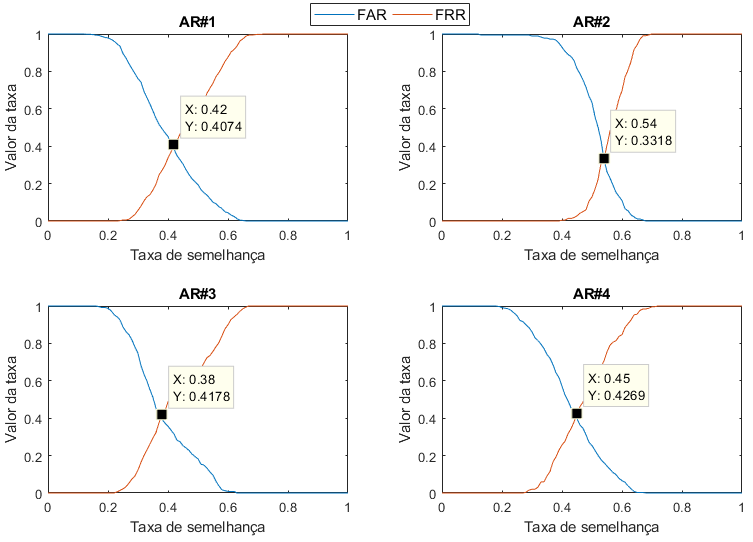
\includegraphics[scale=0.55]{imgs4/graficos_FAR_FRR/APCA}
\label{fig:FAR_FRR_APCA}
\source{Jonas Mendonça Targino, 2018}
\end{figure}


Enquanto na figura \ref{fig:FAR_FRR_fisherfaces} são apresentadas as taxas de FAR e FRR da técnica Fisherfaces nos quatros grupos da base AR. De modo que nos grupos AR\#1, AR\#2, AR\#3 e AR\#4 nos limiares de semelhança iguais a 0.33, 0.36, 0.31 e 0.35 respectivamente as taxas de FAR e FRR se cruzaram, nestes pontos apresentando valores iguais. Portanto, esse limiares de semelhança são os pontos ótimos de aceitação ou rejeição do sistema. 


\begin{figure}[H]
\centering
\caption{Curva com a taxa de falsa aceitação versus taxa de falsa rejeição alcançada pela técnica Fisherfaces}
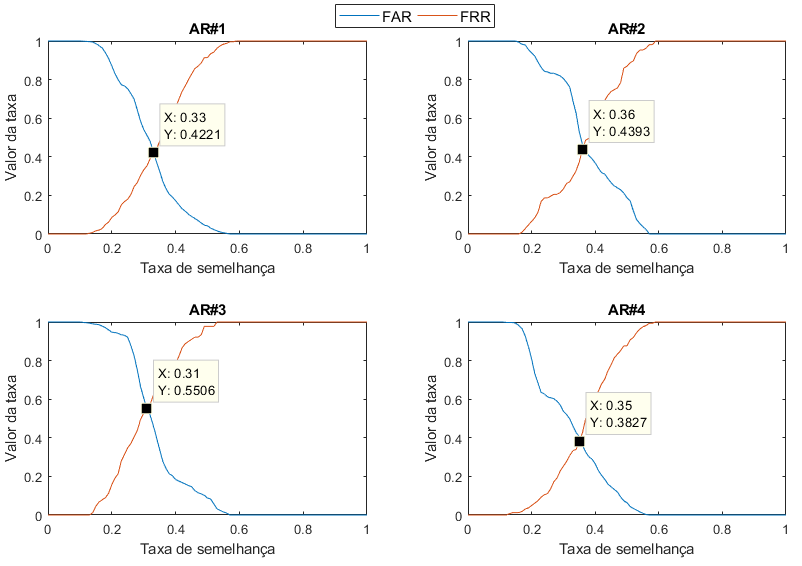
\includegraphics[scale=0.55]{imgs4/graficos_FAR_FRR/fisherfaces}
\label{fig:FAR_FRR_fisherfaces}
\source{Jonas Mendonça Targino, 2018}
\end{figure}


Uma análise similar de FAR e FRR também foi realizada com a técnica Fast Robust PCA. Sendo possível extrair os limiares de semelhança entre a FAR e FRR, sendo eles 0.52, 0.49, 0.58 e 0.49 respectivamente para os grupos AR\#1, AR\#2, AR\#3 e AR\#4. Também é possível perceber o quão alto foi o valor da taxa de FAR e FRR chegando a valores próximos de 0.5 (0.39, 0.42, 0.46 e 0.51) para quase todos os grupos, definindo-se como não sendo uma boa técnica em termos de reconhecimento. Pois quanto menor o valor da taxa, melhor é a técnica.   

\begin{figure}[H]
\centering
\caption{Curva com a taxa de falsa aceitação versus taxa de falsa rejeição alcançada pela técnica Fast Robust PCA}
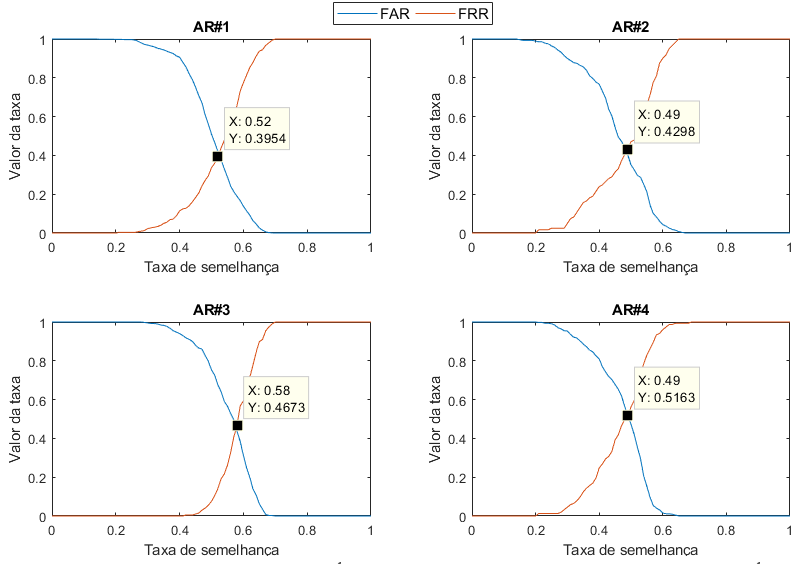
\includegraphics[scale=0.55]{imgs4/graficos_FAR_FRR/FRPCA}
\label{fig:FAR_FRR_FRPCA}
\source{Jonas Mendonça Targino, 2018}
\end{figure}

Enquanto a técnica PCA apresentou taxa de semelhança de FAR e FRR nos pontos 0.45, 0.55, 0.43 e 0.47 para os grupos AR\#1, AR\#2, AR\#3 e AR\#4. Paralelamente apresentando valores de FAR e FRR  nos pontos de cruzamento (0.41, 0.44, 0.48 e 0.40) próximos a 0.5. Sendo 0.5 um valor consideravelmente alto, de modo que é desejável que quanto menor o valor da taxa  de FAR e FRR melhor a técnica para o sistema de reconhecimento. Esses valores estão apresentados conforme a figura \ref{fig:FAR_FRR_PCA}.


\begin{figure}[H]
\centering
\caption{Curva com a taxa de falsa aceitação versus taxa de falsa rejeição alcançada pela técnica PCA}
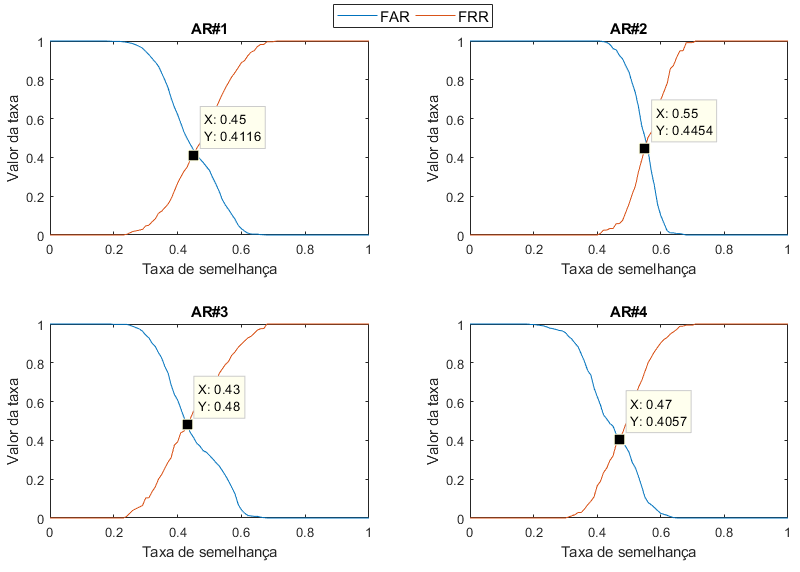
\includegraphics[scale=0.55]{imgs4/graficos_FAR_FRR/PCA}
\label{fig:FAR_FRR_PCA}
\source{Jonas Mendonça Targino, 2018}
\end{figure}


Na análise da técnica Gappy PCA verificou-se os pontos de interseção das curvas de FAR e FRR de 0.5, 0.64, 0.56 e 0.44, de modo que nesses pontos a taxa de semelhança são iguais, conforme ilustra a figura \ref{fig:FAR_FRR_GPCA}. Conforme a figura é possível notar considerável nível de contribuição dessa técnica perante a tarefa de reconstrução.


\begin{figure}[H]
\centering
\caption{Curva com a taxa de falsa aceitação versus taxa de falsa rejeição alcançada pela técnica Gappy PCA}
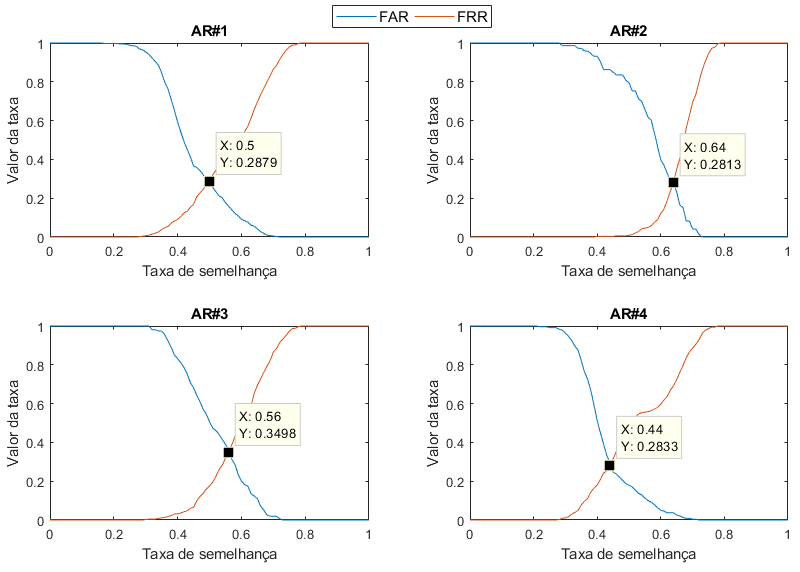
\includegraphics[scale=0.55]{imgs4/graficos_FAR_FRR/GPCA}
\label{fig:FAR_FRR_GPCA}
\source{Jonas Mendonça Targino, 2018}
\end{figure}


Já nas curvas de FAR e FRR da técnica Recursive PCA os pontos 0.48, 0.64, 0.51 e 0.43 dos grupos AR\#1, AR\#2, AR\#3 e AR\#4 respectivamente são os pontos EER, ou seja, são os pontos em que as duas curvas possuem valores iguais, tais resultados estão dispostos na figura \ref{fig:FAR_FRR_Rec_PCA}. Esses sendo os limiares ótimos do algoritmo de acordo com cada grupo. Um fato interessante dessa técnica é que ela foi uma das técnicas baseadas em subespaço que conseguiu os menores valores de taxa de FAR e FRR no ponto de intersecção entre as duas curvas. Desta forma confirmando uma técnica com considerável resultado perante as demais técnicas baseadas em subespaço. Sendo os valores das taxas 0.27, 0.27, 0.22 e 0.29 referentes aos grupos AR\#1, AR\#2, AR\#3 e AR\#4 respectivamente.


\begin{figure}[H]
\centering
\caption{Curva com a taxa de falsa aceitação versus taxa de falsa rejeição alcançada pela técnica Recursive PCA}
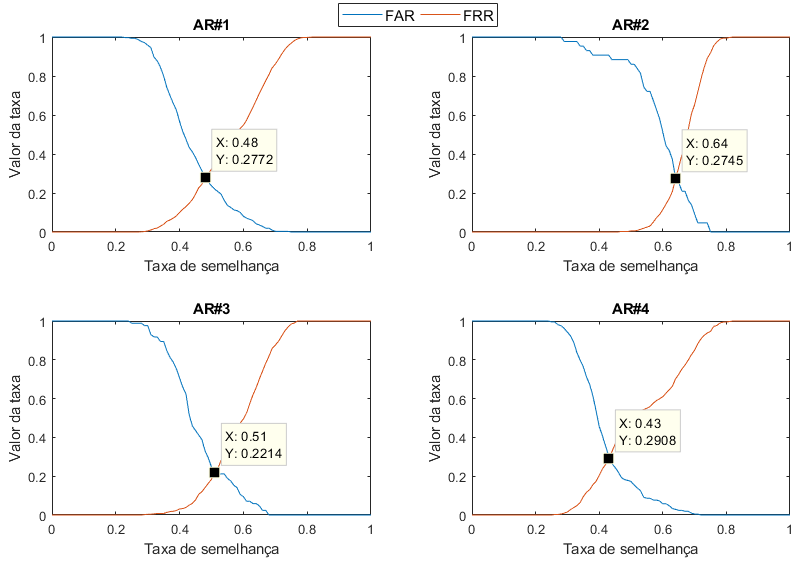
\includegraphics[scale=0.55]{imgs4/graficos_FAR_FRR/RecPCA}
\label{fig:FAR_FRR_Rec_PCA}
\source{Jonas Mendonça Targino, 2018}
\end{figure}


Uma outra técnica baseada em subepaço que apresenta-se promissora é a técnica Fast Recursive PCA, a qual é uma derivação do Recursive PCA, diferenciando-se apenas em sua velocidade de convergência. Ao ser analisada as curvas de FAR e FRR coincidiram com as taxas de FAR e FRR da técnica Recursive PCA. Com isso, demonstrando considerável nível de contribuição dessa técnica quando comparada a outras técnica baseadas em subespaço com mais baixas performances. Tais resultados podem ser visualizados com o auxílio da figura \ref{fig:FAR_FRR_Fast_Rec_PCA}. Essa técnica como também o Recursive PCA atingiram consideráveis performances em todos os guatro grupos, destacando-se um pouco mais nos grupos AR\#2 e AR\#3.


\begin{figure}[H]
\centering
\caption{Curva com a taxa de falsa aceitação versus taxa de falsa rejeição alcançada pela técnica Fast Recursive PCA}
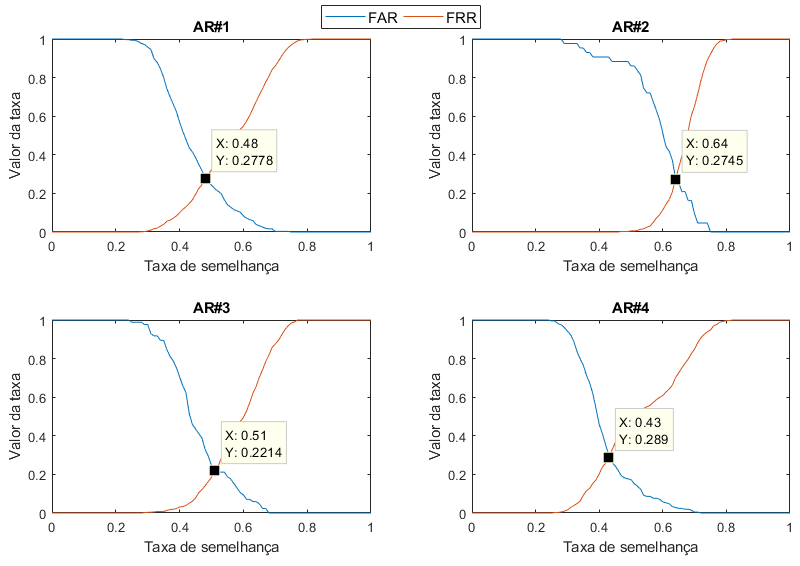
\includegraphics[scale=0.55]{imgs4/graficos_FAR_FRR/FastRecPCA}
\label{fig:FAR_FRR_Fast_Rec_PCA}
\source{Jonas Mendonça Targino, 2018}
\end{figure}

Das técnicas baseadas em subespaço a técnica que apresentou menores pontos de EER foi a técnica desenvolvida nesse trabalho, também intitulada SRC com Fast Recursive PCA. Como podemos ver seus pontos de interseção das duas curvas aconteceu com valores de taxa 0.22, 0.19, 0.18 e 0.28 para os grupos AR\#1, AR\#2, AR\#3 e AR\#4. Tais curvas podem ser visualizadas com o auxílio da figura \ref{fig:FAR_FRR_SRC_Fast_Rec_pca}. A partir da análise da figura é possível perceber bons comportamentos da técnica nos grupos AR\#2 e AR\#3.

\begin{figure}[H]
\centering
\caption{Curva com a taxa de falsa aceitação versus taxa de falsa rejeição alcançada pela técnica SRC com Fast Recursive PCA}
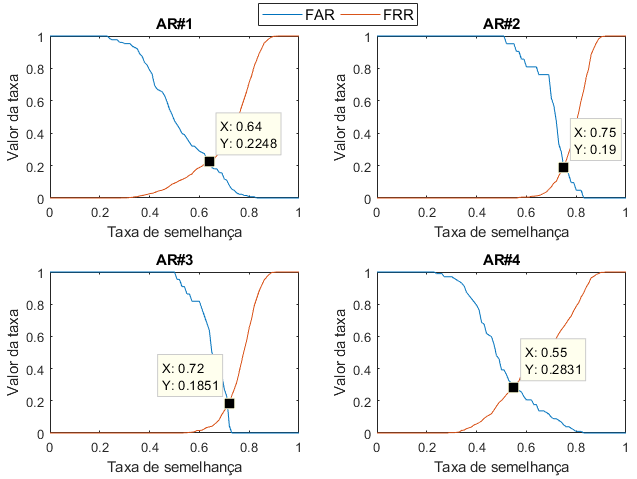
\includegraphics[scale=0.60]{imgs4/graficos_FAR_FRR/src_recPca}
\label{fig:FAR_FRR_SRC_Fast_Rec_pca}
\source{Jonas Mendonça Targino, 2018}
\end{figure}


Deste modo, podemos concluir que das técnicas baseadas em subespaço a técnica SRC Fast Rec PCA foi a técnica que apresentou melhores curvas de FAR e FRR.

Dado que ao analisar as curvas de FAR e FRR, e os pontos EER para cada grupo sobre as técnicas de subespaço apresentadas. Dessa forma vale analisar o comportamento da performance da técnica após aplicação do limiar EER nos respectivos grupos. Com isso foram analisados os comportamentos das quatro melhores técnicas baseadas em subespaço, os quais estão dispostos na tabela \ref{tab:eer_subespaco}, sendo possível perceber que em alguns casos houve uma redução da acurácia após aplicação do limiar.



\begin{table}[htpb]
    \centering
    \footnotesize
	\caption{Análise da técnica após aplicação do limiar EER com classificador ELM}
\begin{tabular}{|c|c|c|c|c|c|c|c|c|}
\hline
\multirow{2}{*}{\textbf{Grupo}}  & \multicolumn{2}{c|}{\textbf{Fast Rec PCA}} & \multicolumn{2}{c|}{\textbf{Gappy PCA}}  & \multicolumn{2}{c|}{\textbf{Recursive PCA}}  & \multicolumn{2}{c|}{\textbf{SRC Fast PCA}}  \\\cline{2-9}
 & \textbf{Normal} & \textbf{EER}& \textbf{Normal} & \textbf{EER} & \textbf{Normal} & \textbf{EER} & \textbf{Normal} & \textbf{EER} \\\hline

AR\#1 &	74.08\%	& 74.08\%	&64.25\%	& 64.16\%	&74.25\%	&74.25\% & 89.33\%	&89.33\% \\\hline
AR\#2 &	89.25\%	& 89.25\%	&81.75\%	& 81.75\%	&89.25\%	&89.25\% & 94.75\%	&94.75\% \\\hline
AR\#3 &	85.83\%	& 85.83\%	&74.33\%	& 73.66\%	&85.83\%	&85.83\% & 96.33\%	&96.33\% \\\hline
AR\#4 &	65.16\%	& 64.83\%	&60.00\%	& 59.83\%	&65.33\%	&64.66\% & 83.00\%	&83.00\% \\\hline
 \end{tabular}
\label{tab:eer_subespaco}
\end{table}




%A fins de detalhes sobre erros por classe de cada técnica, foram disponibilizadas as matrizes de confusão de cada técnica, tais matrizes  encontram-se disponíveis no apêndice \ref{Apen:matrizes_confusao}. 



\subsection{Resultados das técnicas baseadas em subespaço nos grupos da base Yale}

Ao utilizar as técnicas baseadas em subespaço nos dois grupos da base Yale foram vistos resultados similares de reconstrução aos apresentados nos quatro grupos da base AR. Tais resultados de reconstrução são apresentados na figura \ref{fig:reconstrucao_subespaco_yale}. Nesta figura é possível perceber que as técnicas que apresentaram melhores imagens reconstruídas em nível de percepção visual foram as técnicas SRC Fast Rec PCA, Rec PCA, Fast Rec PCA e GPCA.

\begin{figure}[H]
\centering
\caption{Imagens reconstruídas com as técnicas baseadas em subespaço nos grupos da base Yale}
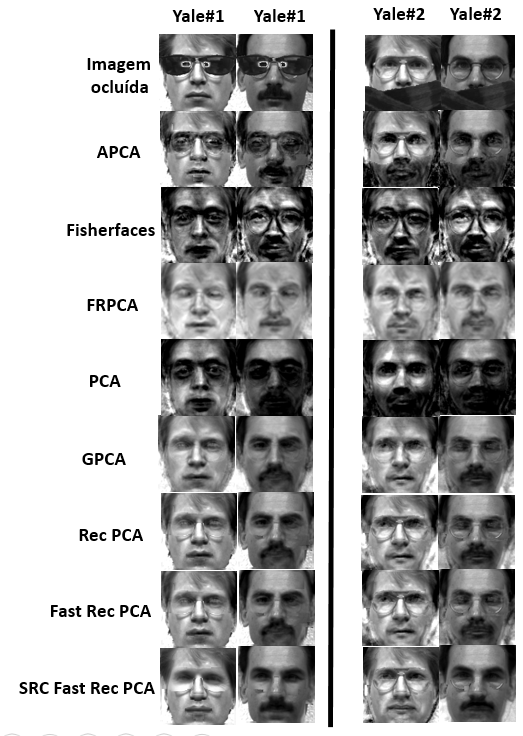
\includegraphics[scale=0.70]{imgs4/reconstrucoes_subespaco_yale}
\label{fig:reconstrucao_subespaco_yale}
\source{Jonas Mendonça Targino, 2018}
\end{figure}

Paralelamente também foram analisadas algumas métricas de validação das imagens reconstruídas. Sendo utilizadas as métricas RMSE, PSNR e SSIM. Na tabela \ref{tab:RMSE_subespaco_Yale} são apresentados os valores de RMSE de cada técnica por grupo. Nessa tabela é possível perceber que o melhor resultado de RMSE para  os dois grupos foram obtidos com a técnica SRC Fast Rec PCA. De todas as técnicas a técnica PCA foi a  técnica que apresentou maiores valores de RMSE.

\begin{table}[H]
\caption{Resultados de RMSE das técnicas baseadas em subespaço nos grupos da base Yale}
\centering
\begin{tabular}{|c|c|c|}
\cline{2-3}
 \multicolumn{1}{c|}{} & \multicolumn{2}{c|}{\textbf{RMSE}}\\ \hline
\multicolumn{1}{|c|}{\multirow{2}{*}{\textbf{Técnica} }}& \textbf{Yale\#1} &  \textbf{Yale\#2}   \\ \cline{2-3}

& média $\pm$ desvio & média $\pm$ desvio \\\hline 
APCA&	        58.65$\pm$9.85	&78.79$\pm$11.82 \\\hline
FRPCA&	        61.80$\pm$15.19	&59.12$\pm$14.54\\\hline
Fast Rec PCA&	53.01$\pm$10.70 &58.90$\pm$9.85\\\hline
Fisherfaces&	71.29$\pm$12.63 &80.53$\pm$9.54\\\hline
GPCA	    &   52.26$\pm$10.52	&54.61$\pm$9.81\\\hline
PCA	         &  75.81$\pm$17.59	&92.79$\pm$17.89\\\hline
Recursive PCA&	53.19$\pm$10.55	&54.84$\pm$10.03\\\hline
SRC Fast Rec PCA &	\textbf{51.08$\pm$12.73}	&\textbf{52.28$\pm$11.26}\\\hline

\end{tabular}
\source{Jonas Mendonça Targino, 2018}
\label{tab:RMSE_subespaco_Yale}
\end{table}

Resultados similares nesses dois grupos também foram obtidos com a métrica PSNR, em que a técnica SRC Fast Rec PCA novamente apresentou os melhores resultados. Tais observações podem ser visualizadas com o auxílio da tabela \ref{tab:PSNR_subespaco_Yale}.

\begin{table}[H]
\caption{Resultados de PSNR das técnicas baseadas em subespaço nos grupos da base Yale}
\centering
\begin{tabular}{|c|c|c|}
\cline{2-3}
 \multicolumn{1}{c|}{} & \multicolumn{2}{c|}{\textbf{PSNR}}\\ \hline
\multicolumn{1}{|c|}{\multirow{2}{*}{\textbf{Técnica} }}& \textbf{Yale\#1} &  \textbf{Yale\#2}   \\ \cline{2-3}

& média $\pm$ desvio & média $\pm$ desvio \\\hline 
APCA&	        12.87$\pm$1.44&	10.28$\pm$1.28\\\hline
FRPCA&	        12.56$\pm$2.20&	12.93$\pm$2.11\\\hline
Fast Rec PCA&	13.81$\pm$1.80&	12.83$\pm$1.40\\\hline
Fisherfaces&	11.19$\pm$1.51&	10.06$\pm$1.02\\\hline
GPCA&       	13.93$\pm$1.81&	13.52$\pm$1.65\\\hline
PCA&            10.72$\pm$1.81&	8.93$\pm$1.70\\\hline
Recursive PCA&	13.78$\pm$1.79&	13.49$\pm$1.68\\\hline
SRC Fast Rec PCA&	\textbf{14.23$\pm$2.29}&	\textbf{13.94$\pm$1.81}\\\hline
\end{tabular}
\source{Jonas Mendonça Targino, 2018}
\label{tab:PSNR_subespaco_Yale}
\end{table}

Ao analisar a métrica SSIM nos dois grupos da base Yale, podemos perceber os melhores resultados com a técnica SRC Fast Rec PCA, seguidamente das técnicas GPCA, Rec PCA e Fast Rec PCA, conforme demonstrado na tabela \ref{tab:SSIM_subespaco_Yale}


\begin{table}[H]
\caption{Resultados de SSIM das técnicas baseadas em subespaço nos grupos da base Yale}
\centering
\begin{tabular}{|c|c|c|}
\cline{2-3}
 \multicolumn{1}{c|}{} & \multicolumn{2}{c|}{\textbf{SSIM}}\\ \hline
\multicolumn{1}{|c|}{\multirow{2}{*}{\textbf{Técnica} }}& \textbf{Yale\#1} &  \textbf{Yale\#2}   \\ \cline{2-3}

& média $\pm$ desvio & média $\pm$ desvio \\\hline 
APCA        	&0.40$\pm$0.04& 	0.34$\pm$0.04\\\hline
FRPCA       	&0.49$\pm$0.05&	    0.49$\pm$0.06\\\hline
Fast Rec PCA	&0.48$\pm$0.04&	    0.41$\pm$0.05\\\hline
Fisherfaces 	&0.23$\pm$0.05& 	0.18$\pm$0.03\\\hline
GPCA	        &0.50$\pm$0.04&	    0.46$\pm$0.05\\\hline
PCA	            &0.29$\pm$0.04& 	0.24$\pm$0.04\\\hline
Recursive PCA   &0.48$\pm$0.04&	    0.44$\pm$0.05\\\hline
SRC Fast Rec PCA     &0.51$\pm$0.07&	    0.48$\pm$0.06\\\hline

\end{tabular}
\source{Jonas Mendonça Targino, 2018}
\label{tab:SSIM_subespaco_Yale}
\end{table}

Ao analisar a acurácia das técnicas baseadas em subespaço nos dois grupos de oclusões da base Yale, verificou-se maiores dificuldades de reconhecimento no grupo Yale\#2, visto que as técnicas SRC Fast Rec PCA, Rec PCA, Fast Rec PCA e GPCA apresentaram os melhores resultados de reconhecimento no grupo Yale\#2 da base Yale. Enquanto a base ocluída conseguiu 100\% de acurácia no grupo Yale\#1, este grupo sendo definido como um grupo de oclusões que não implicam diretamente na taxa de reconhecimento. Considerando-se como um grupo que não necessita do processo de reconstrução. Tais resultados podem ser visualizados com o auxílio da figura \ref{fig:acuracia_yale_subespaco_KNN}.

\begin{figure}[H]
\centering
\caption{Acurácia com KNN com nível 3 de decomposição da TW  nos dois grupos da base Yale}
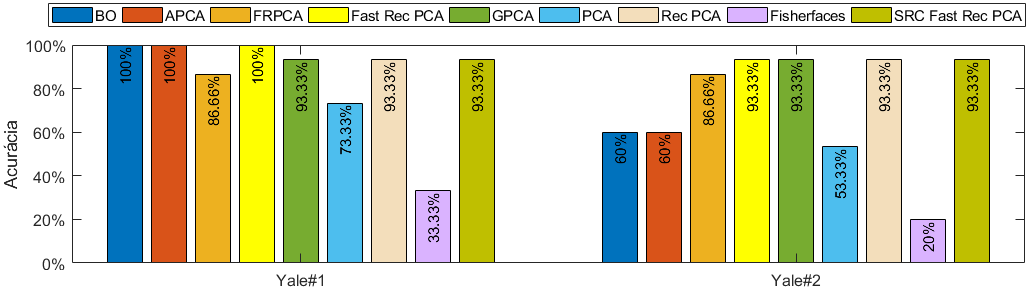
\includegraphics[scale=0.55]{imgs4/acuracia/acuracia_Yale_subespaco_KNN}
\source{Jonas Mendonça Targino, 2018}
\label{fig:acuracia_yale_subespaco_KNN}
\end{figure}

Da mesma forma ao se analisar as técnicas com classificador ELM é possível perceber que as técnicas baseadas em subespaço Fast Rec PCA, Rec PCA e GPCA apresentaram 100\% de reconhecimento para os dois grupos da base Yale. Justificando-se como ótimas técnicas quando apresentadas a bases de dados com baixo número de indivíduos. A figura \ref{fig:acuracia_yale_subespaco_ELM} ilustra o comportamento das técnicas baseadas em  subespaço ao serem apresentadas com os dois grupos da base Yale.

\begin{figure}[H]
\centering
\caption{Acurácia com ELM com nível 3 de decomposição da TW nos dois grupos da base Yale}
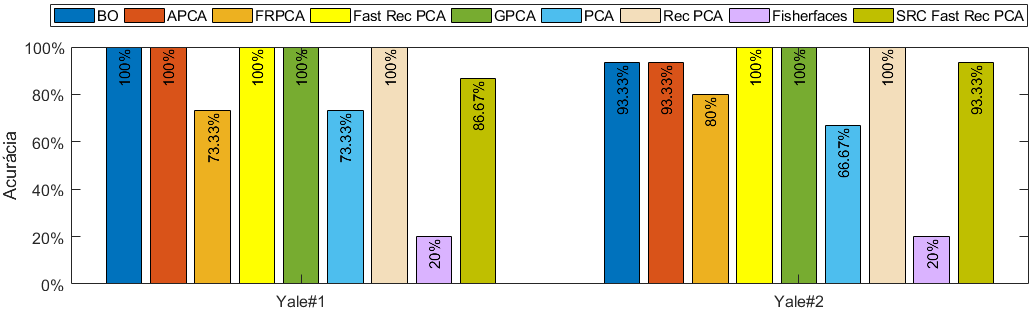
\includegraphics[scale=0.55]{imgs4/acuracia/acuracia_Yale_subespaco_ELM}
\source{Jonas Mendonça Targino, 2018}
\label{fig:acuracia_yale_subespaco_ELM}
\end{figure}


Enquanto ao avaliar-se os mesmos grupos com SVM conseguiu-se 100\% de taxa de reconhecimento em quase todas as técnicas exceto com SRC Fast Rec PCA, Fisherfaces e PCA os quais apresentaram resultados inferiores de acurácia. Como ilustrado na figura \ref{fig:acuracia_yale_subespaco_SVM}.


\begin{figure}[H]
\centering
\caption{Acurácia com SVM com nível 3 de decomposição da TW nos dois grupos da base Yale}
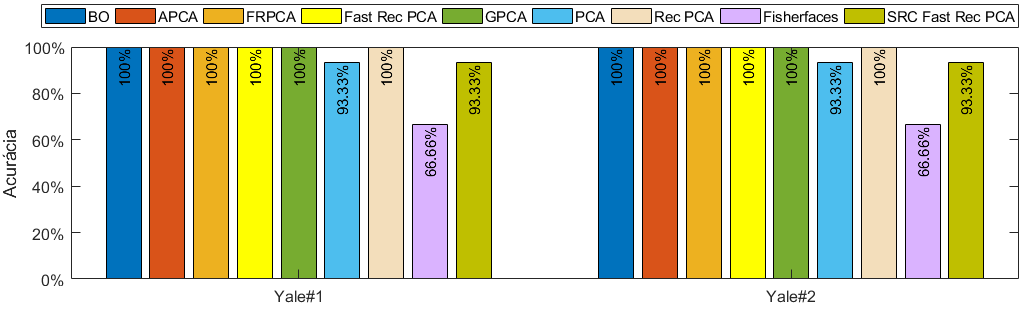
\includegraphics[scale=0.55]{imgs4/acuracia/acuracia_Yale_subespaco_SVM}
\source{Jonas Mendonça Targino, 2018}
\label{fig:acuracia_yale_subespaco_SVM}
\end{figure}

Dado que a maioria das técnicas baseadas em subespaço apresentaram bons resultados na base Yale, aqui são apresentados apenas os resultados do terceiro nível de decomposição da TW.







\section{Resultados das técnicas baseadas em modelo}

De modo a identificar todas as técnicas baseadas em modelo foram criadas algumas abreviações para as técnicas de modo a realizar o posicionamento de maneira satisfatória frente a leitura do texto. Essas abreviações estão dispostas na tabela \ref{tab:tecnicas_modelo}.

\begin{table}[htpb]
	\centering
	\caption{Abreviações geradas para as três técnicas baseadas em modelo}
    \label{tab:tecnicas_modelo}
    %\space
	\begin{tabular}{|l|c|} \hline

		\textbf{Técnica}	& Abreviação  \\ \hline
		SRC GP  & SRC com grafo de Poisson  \\ \hline
		SRC GL  & SRC com grafo Laplaciano  \\ \hline
		SSIMGL & Similaridade Estrutural com grafo Laplaciano \\ \hline
		 
	\end{tabular}
\source{Jonas Mendonça Targino, 2018}
\end{table}

Após a reconstrução das imagens dos seis grupos nas duas bases de dados com as técnicas baseadas em modelo chegou-se aos resultados de reconstrução que serão apresentados logo abaixo.

\subsection{Resultados nos quatro grupos da base AR}

Na figura \ref{fig:exemplos_rec_modelo} são apresentadas oito imagens reconstruídas de dois indivíduos sobre os quatro grupos da base AR com as três técnicas baseadas em modelo, com a ajuda da figura é possível perceber imagens reconstruídas com poucos ruídos, implicando-se em boas técnicas de reconstrução.

\begin{figure}[H]
\centering
\caption{Exemplos de imagens de dois individuos reconstruídas com as técnicas baseadas em modelo}
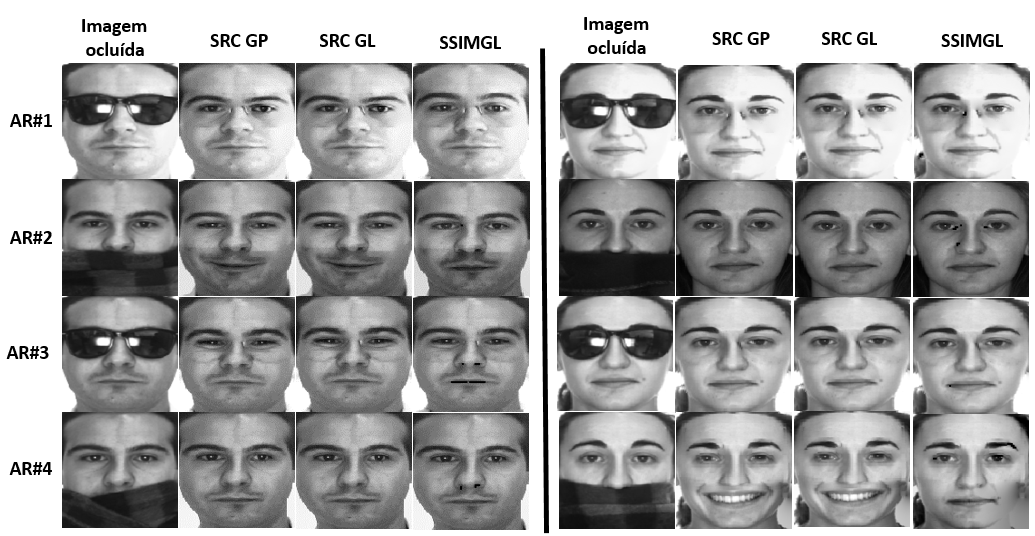
\includegraphics[scale=0.55]{imgs4/reconstrucoes_modelo}
\source{Jonas Mendonça Targino, 2018}
\label{fig:exemplos_rec_modelo}
\end{figure}


Ao analisarmos as métricas de qualidade das imagens reconstruídas podemos perceber que a técnica SSIMGL foi a técnica que apresentou menores médias de erro (RMSE) para os quatro grupos presentes na base AR, conforme apresentado na tabela \ref{tab:RMSE_modelo}. Podemos perceber também com o auxílio dessa tabela que a segunda melhor técnica baseada em modelo foi a técnica SRC GL.

\begin{table}[H]
\caption{Resultados de RMSE das técnicas baseadas em modelo}
\centering
\begin{tabular}{|c|c|c|c|c|}
\cline{2-5}
 \multicolumn{1}{c|}{} & \multicolumn{4}{c|}{\textbf{RMSE}}\\ \hline
\multicolumn{1}{|c|}{\multirow{2}{*}{\textbf{Técnica} }}& \textbf{AR\#1} &  \textbf{AR\#2} & \textbf{AR\#3} & \textbf{AR\#4 }  \\ \cline{2-5}
& média $\pm$ desvio & média $\pm$ desvio & média $\pm$ desvio & média $\pm$ desvio \\\hline 
SRC GP&	51.21$\pm$18.45&	29.61$\pm$12.28&	51.58$\pm$19.74& 	50.84$\pm$17.07 \\\hline
SRC GL&	51.17$\pm$18.47&	29.59$\pm$12.56&	51.42$\pm$19.81&	50.91$\pm$17.04 \\\hline
SSIMGL&	49.53$\pm$17.65&	28.64$\pm$11.40&	50.96$\pm$19.33&	48.09$\pm$15.68 \\\hline
\end{tabular}
\source{Jonas Mendonça Targino, 2018}
\label{tab:RMSE_modelo}
\end{table}


Resultados similares foram obtidos ao avaliarmos a métrica PSNR, de modo que a técnica SSIMGL apresentou os maiores valores de PSNR para os quatro grupos. Vindo a alcançar uma média de $19.33$ para o grupo AR\#2, conforme a tabela \ref{tab:PSNR_modelo}.

\begin{table}[H]
\caption{Resultados de PSNR das técnicas baseadas em modelo}
\centering
\begin{tabular}{|c|c|c|c|c|}
\cline{2-5}
 \multicolumn{1}{c|}{} & \multicolumn{4}{c|}{\textbf{PSNR}}\\ \hline
\multicolumn{1}{|c|}{\multirow{2}{*}{\textbf{Técnica} }}& \textbf{AR\#1} &  \textbf{AR\#2} & \textbf{AR\#3} & \textbf{AR\#4 }  \\ \cline{2-5}
& média $\pm$ desvio & média $\pm$ desvio & média $\pm$ desvio & média $\pm$ desvio \\\hline 
SRC GP	&14.38$\pm$4.18&	19.12$\pm$3.72&	14.43$\pm$4.46&	14.34$\pm$3.88\\\hline
SRC GL	&14.40$\pm$4.21&	19.16$\pm$3.79&	14.48$\pm$4.52&	14.32$\pm$3.88\\\hline
SSIMGL	&14.64$\pm$4.05&	19.33$\pm$3.47&	14.51$\pm$4.35&	14.78$\pm$3.74\\\hline
\end{tabular}
\source{Jonas Mendonça Targino, 2018}
\label{tab:PSNR_modelo}
\end{table}

Ao analisarmos a métrica SSIM é possível perceber que novamente a métrica SSIMGL apresentou melhores resultados, conforme podemos visualizar na tabela \ref{tab:SSIM_modelo}. Chegando a obter 0.74 de SSIM no grupo AR\#2.


\begin{table}[H]
\caption{Resultados de SSIM das técnicas baseadas em modelo}
\centering
\begin{tabular}{|c|c|c|c|c|}
\cline{2-5}
 \multicolumn{1}{c|}{} & \multicolumn{4}{c|}{\textbf{SSIM}}\\ \hline
\multicolumn{1}{|c|}{\multirow{2}{*}{\textbf{Técnica} }}& \textbf{AR\#1} &  \textbf{AR\#2} & \textbf{AR\#3} & \textbf{AR\#4 }  \\ \cline{2-5}
& média $\pm$ desvio & média $\pm$ desvio & média $\pm$ desvio & média $\pm$ desvio \\\hline 
SRC GP&	0.62$\pm$0.11	&0.71$\pm$0.11&	0.65$\pm$0.10&	0.59$\pm$0.11\\\hline
SRC GL&	0.62$\pm$0.11	&0.72$\pm$0.11&	0.65$\pm$0.10&	0.59$\pm$0.11\\\hline
SSIMGL&	0.64$\pm$0.11	&0.74$\pm$0.11&	0.66$\pm$0.10&	0.63$\pm$0.11\\\hline
\end{tabular}
\source{Jonas Mendonça Targino, 2018}
\label{tab:SSIM_modelo}
\end{table}


Ao analisar o desempenho das técnicas baseadas em modelo com classificador KNN utilizando a decomposição LL nível 3 foi possível perceber melhores resultados com a técnica SSIMGL para os quatro grupos da base AR. De modo que os melhores resultados foram alcançados nos grupos AR\#2 e AR\#3 para as três técnicas baseadas em modelo. Em que podemos perceber ganhos significativos de 42.75\%, 49.75\%, 18.84\% e 66.50\% para os grupos AR\#1, AR\#2, AR\#3 e AR\#4 respectivamente com a técnica SSIMGL. Percebendo maior ganho pela técnica SSIMGL no grupo AR\#4. Também é interessante analisar comportamentos bem próximos das técnicas baseadas em SRC, de modo que a SRC GL quando comparada ao SRC GP não apresentou percentuais de diferença de acurácia maior que 3\% entre as duas técnicas. A figura \ref{fig:acuracia_modelo_KNN} ilustra tal comportamento.


\begin{figure}[H]
\centering
\caption{Acurácia das técnicas baseadas em modelo com classificador KNN com nível de decomposição 3 da TW nos quatro grupos presentes na base AR}
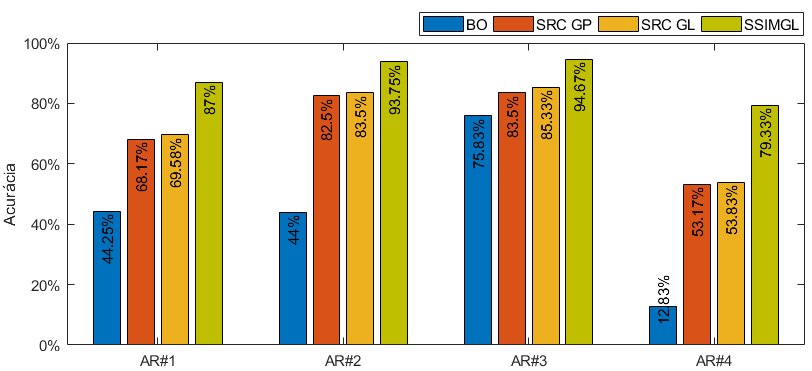
\includegraphics[scale=0.52]{imgs4/acuracia_modelo_KNN}
\label{fig:acuracia_modelo_KNN}
\source{Jonas Mendonça Targino, 2018}
\end{figure}

Enquanto ao utilizarmos o nível 2 de decomposição  a técnica SSIMGL apresentou melhores resultados de taxa de acurácia em 3 dos 4 grupos da base AR, de modo que a técnica SSIMGL conseguiu quase 4\% a mais de taxa de acurácia no grupo AR\#4 ao utilizar o nível 2, conforme ilustra a figura \ref{fig:acuracia_modelo_KNN_nivel2}. 

\begin{figure}[H]
\centering
\caption{Acurácia das técnicas baseadas em modelo com classificador KNN com nível de decomposição 2 da TW nos quatro grupos presentes na base AR}
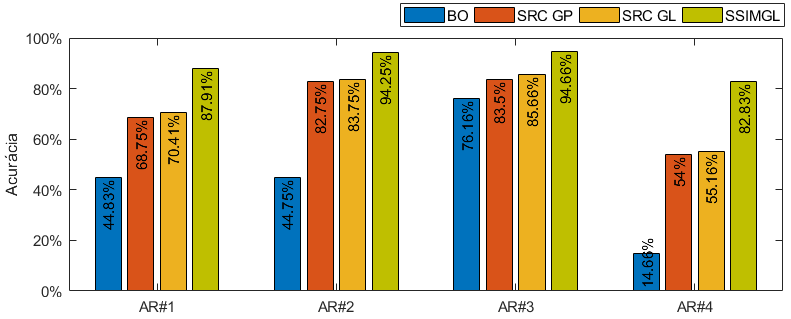
\includegraphics[scale=0.52]{imgs4/acuracia/nivel_one_two/knn_nivel2_modelo}
\label{fig:acuracia_modelo_KNN_nivel2}
\source{Jonas Mendonça Targino, 2018}
\end{figure}


Com classificador KNN e nível 1 de decomposição foi possível perceber que não houve ganho de performance ao  aumentar o número de características de modo que todas as três técnicas baseadas em modelo apresentaram resultados inferiores quando comparada com os resultados obtidos com nível 2 de decomposição com o mesmo classificador. Tais resultados podem ser confirmados com o auxílio da figura \ref{fig:acuracia_modelo_KNN_nivel1}.


\begin{figure}[H]
\centering
\caption{Acurácia das técnicas baseadas em modelo com classificador KNN com nível 1 de decomposição da TW nos quatro grupos presentes na base AR}
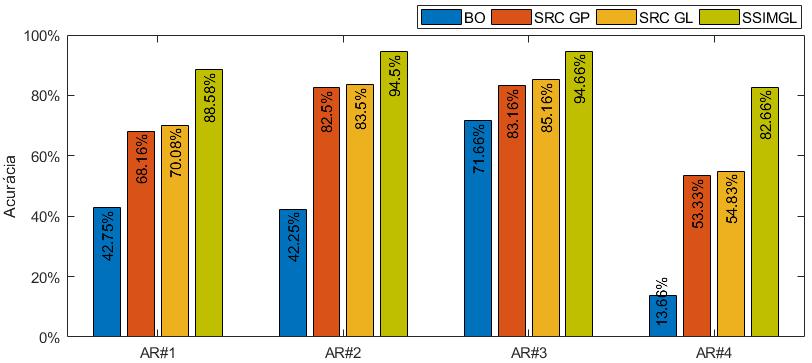
\includegraphics[scale=0.52]{imgs4/acuracia/nivel_one_two/knn_nivel1_modelo}
\label{fig:acuracia_modelo_KNN_nivel1}
\source{Jonas Mendonça Targino, 2018}
\end{figure}


Resultados superiores aos apresentados com KNN, são perceptíveis com classificador ELM. Em que a ELM obteve ganhos de acurácia de 47.07\%, 40.08 \%, 45.49\% e 47.29\% respectivamente para os grupos AR\#1, AR\#2, AR\#3 e AR\#4 utilizando o nível 3 de decomposição com a técnica SSIMGL. Enquanto as técnicas SRC GP e SRC apresentaram resultados de acurácia muito próximos, de modo que a técnica SRC GL obteve resultados um pouco melhores em que os mesmos não ultrapassaram 3\% de acurácia superior a técnica SRC GP. Tais resultados podem ser visualizados com o auxílio da figura \ref{fig:acuracia_modelo_ELM}.



\begin{figure}[H]
\centering
\caption{Acurácia das técnicas baseadas em modelo com classificador ELM com nível 3 de decomposição da TW nos quatro grupos presentes na base AR}
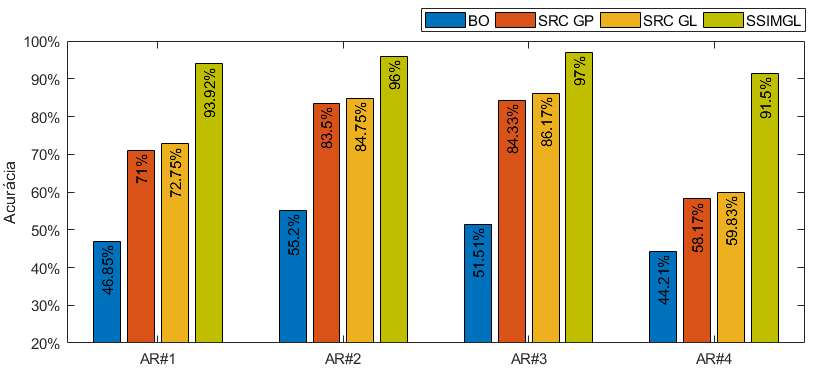
\includegraphics[scale=0.52]{imgs4/acuracia_modelo_ELM}
\label{fig:acuracia_modelo_ELM}
\source{Jonas Mendonça Targino, 2018}
\end{figure}


Enquanto ao utilizar o nível 2 de decomposição da TW com classificador ELM a técnica SSIMGL novamente conseguiu as melhores taxas de reconhecimento, entretanto nos grupos AR\#2 e AR\#3 houve uma queda de performance de 96\% para 95.75\% e 97\% para 96.33\% nos respectivos grupos, conforme ilustra a figura \ref{fig:acuracia_modelo_ELM_nivel2}. Enquanto nos grupos AR\#1 e AR\#4 houve ganho de performance de 93.92\% para 95.17\% e 91.50\% para 94.17\%. Podendo perceber tais ganhos de performances nos grupos com maiores variações de iluminação como também aumento do tamanho da oclusão.


\begin{figure}[H]
\centering
\caption{Acurácia das técnicas baseadas em modelo com classificador ELM com nível 2 de decomposição da TW nos quatro grupos presentes na base AR}
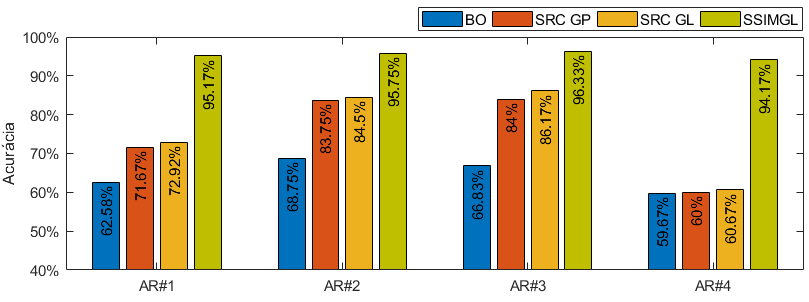
\includegraphics[scale=0.52]{imgs4/acuracia/nivel_one_two/ELM_nivel2_modelo}
\label{fig:acuracia_modelo_ELM_nivel2}
\source{Jonas Mendonça Targino, 2018}
\end{figure}

Novamente a técnica SSIMGL apresentou resultados superiores as técnicas SRC GP e SRC GL ao utilizar nível 1 de decomposição com TW. De modo que não houve ganho significativo ao utilizar o nível 1 de decomposição em relação ao nível 2. Em que podemos perceber resultados próximos de taxa de reconhecimento. Significando-se que o nível 2 apresenta-se muito representativo quando comparado ao nível 1 de decomposição da TW. A figura \ref{fig:acuracia_modelo_ELM_nivel1} ilustra os resultados de acurácia dos métodos baseados em modelo ao utilizar o nível 1 de decomposição.


\begin{figure}[H]
\centering
\caption{Acurácia das técnicas baseadas em modelo com classificador ELM com nível 1 de decomposição da TW nos quatro grupos presentes na base AR}
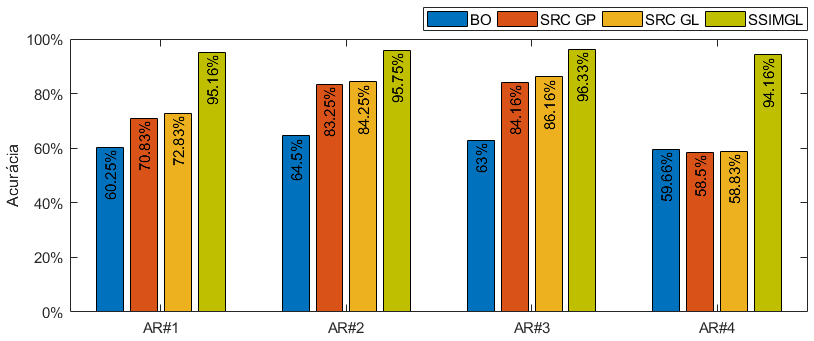
\includegraphics[scale=0.52]{imgs4/acuracia/nivel_one_two/ELM_nivel1_modelo}
\label{fig:acuracia_modelo_ELM_nivel1}
\source{Jonas Mendonça Targino, 2018}
\end{figure}


Ao utilizar o classificador SVM com nível 3 de decomposição da TW nos quatro grupos da base AR podemos perceber consideráveis percentuais de acurácia da técnica SSIMGL, apresentando resultados superiores as demais técnicas baseadas em modelo. Obtendo ganhos de reconstrução de 31.33\%, 25.75\%, 3.83\% e 22.00\% respectivamente nos grupos AR\#1, AR\#2, AR\#3 e AR\#4 com a técnica SSIMGL. Um fato interessante do classificador SVM nesses conjuntos é que ao lidar com oclusões de óculos no grupo AR\#3, mesmo com a base ocluída nesse grupo ele conseguiu 92.83\% de acurácia, conforme a figura \ref{fig:acuracia_modelo_SVM}. 

\begin{figure}[H]
\centering
\caption{Acurácia das técnicas baseadas em modelo com classificador SVM com nível 3 de decomposição da TW nos quatro grupos presentes na base AR}
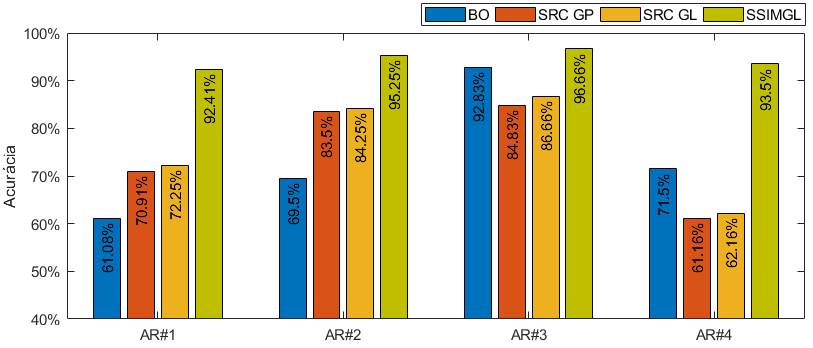
\includegraphics[scale=0.52]{imgs4/acuracia_modelo_SVM}
\label{fig:acuracia_modelo_SVM}
\source{Jonas Mendonça Targino, 2018}
\end{figure}


Paralelamente ao utilizar o nível 2 da TW com classificador SVM foi possível obter ganhos de performance quando comparada ao SVM com nível 3 de decomposição com os grupos AR\#1 e AR\#4 utilizando a técnica SSIMGL como base, sendo a técnica que apresentou melhores resultados. Enquanto no grupo AR\#2 a performance manteve-se contínua. Já no grupo AR\#3 teve-se uma pequena queda de performance de 96.66\% para 96.50\%. Tais resultados podem ser visualizados com o auxílio da figura \ref{fig:acuracia_modelo_SVM_nivel2}.

\begin{figure}[H]
\centering
\caption{Acurácia das técnicas baseadas em modelo com classificador SVM com nível 2 de decomposição da TW nos quatro grupos presentes na base AR}
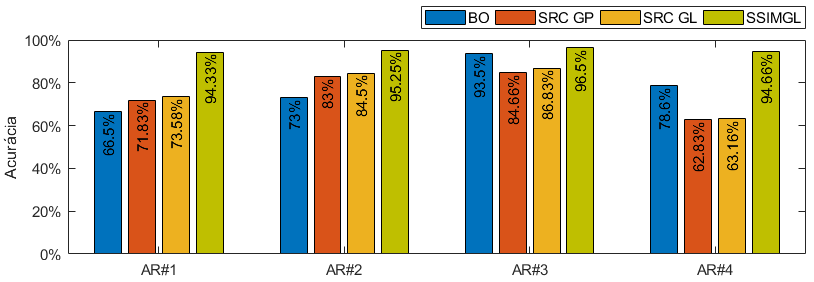
\includegraphics[scale=0.52]{imgs4/acuracia/nivel_one_two/SVM_nivel2_modelo}
\label{fig:acuracia_modelo_SVM_nivel2}
\source{Jonas Mendonça Targino, 2018}
\end{figure}


%\begin{figure}[H]
%\centering
%\caption{Acurácia das técnicas baseadas em modelo com classificador SVM com nível 1 de decomposição da TW nos quatro grupos presentes na base AR}
%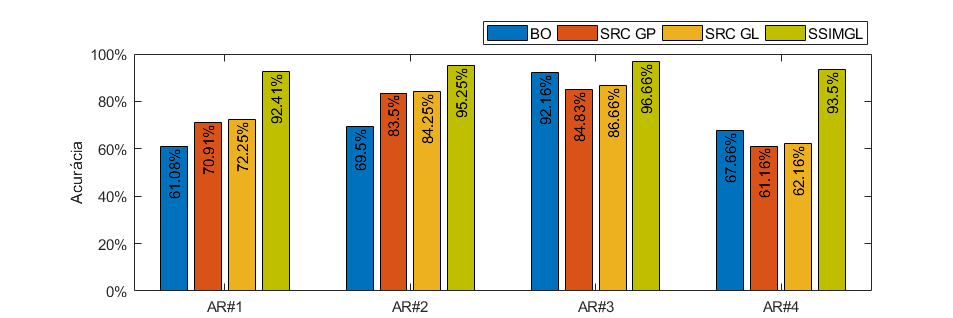
\includegraphics[scale=0.52]{imgs4/acuracia/nivel_one_two/SVM_nivel1_modelo}
%\label{fig:acuracia_modelo_SVM_nivel1}
%\source{Jonas Mendonça Targino, 2018}
%\end{figure}


Ao analisar o ganho ao utilizar os níveis de decomposição 1, 2 e 3 podemos perceber que com a avaliação com classificador KNN o nível 3 de decomposição representa muito bem todo  o conjunto de modo que não há ganho significativo ao utilizar os níveis 1 e 2. A figura \ref{fig:acuracia_ganho_modelo_KNN} ilustra os ganhos das técnicas baseadas em modelo ao se utilizar os três níveis de decomposição da TW com classificador KNN.

\begin{figure}[H]
\centering
\caption{Ganho das técnicas baseadas em modelo ao utilizar os níveis 1 e 2 de decomposição da TW com classificador KNN }
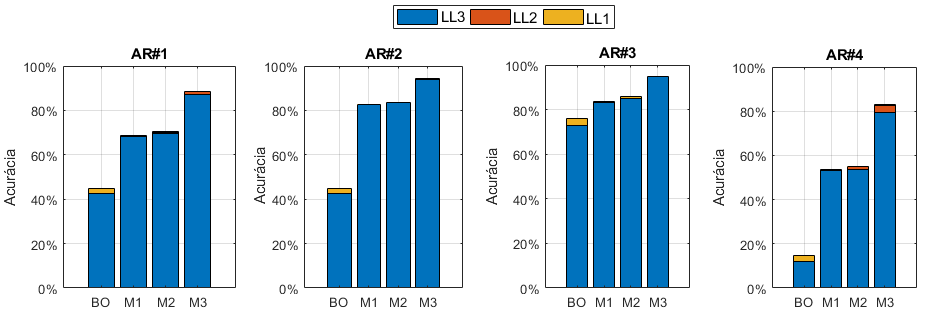
\includegraphics[scale=0.52]{imgs4/ganhos/ganho_modelo_KNN_niveis}
\label{fig:acuracia_ganho_modelo_KNN}
\source{Jonas Mendonça Targino, 2018}
\end{figure}

Enquanto ao avaliarmos cada técnica com classificador ELM nos três níveis de decomposição podemos perceber ganho significativo ao utilizar os níveis 1 e 2 apenas para a base ocluída. Enquanto para as técnicas baseadas em modelo existe baixo ganho ao utilizar os níveis 1 e 2. A figura \ref{fig:acuracia_ganho_modelo_ELM} ilustra o ganho das técnicas baseadas em modelo após utilizar os três níveis de decomposição com TW. 

\begin{figure}[H]
\centering
\caption{Ganho das técnicas baseadas em modelo ao utilizar os níveis 1 e 2 de decomposição da TW com classificador ELM }
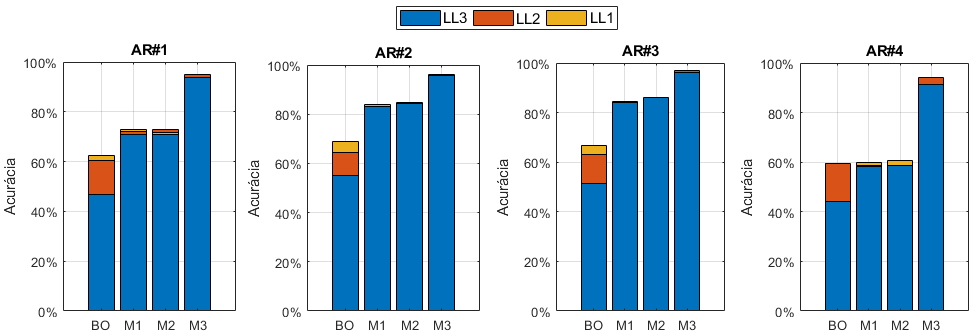
\includegraphics[scale=0.52]{imgs4/ganhos/ganho_modelo_ELM_niveis}
\label{fig:acuracia_ganho_modelo_ELM}
\source{Jonas Mendonça Targino, 2018}
\end{figure}


Resultados similares aos resultados dos ganhos com ELM podem ser visualizados com o classificador SVM utilizando o nível 2 de decomposição conforme ilustra a figura \ref{fig:acuracia_ganho_modelo_SVM}, em que podemos visualizar maior ganho apenas ao se avaliar a base ocluída. Induzindo-se que o nível 3 decomposição apresenta boa representatividade de todo o conjunto.

\begin{figure}[H]
\centering
\caption{Ganho das técnicas baseadas em modelo ao utilizar o nível 2 de decomposição da TW com classificador SVM }
\includegraphics[scale=0.52]{imgs4/ganhos/ganho_modelo_SVM_niveis}
\label{fig:acuracia_ganho_modelo_SVM}
\source{Jonas Mendonça Targino, 2018}
\end{figure}



Quando analisamos as técnicas de reconstrução também é interessante analisarmos o erro por classe dessa técnica, de modo a analisar qual indivíduo o classificador errou mais, como também verificar qual indivíduo o classificador julgou ser erroneamente. Tais análises são interessantes de modo a conhecer características similares entre tais indivíduos.


Ao se analisar o erro por classe da técnica SRC GP foram visualizadas maiores variações nos grupos AR\#1 e AR\#4, conforme a figura \ref{fig:taxa_erro_REC_SRC_Poisson}. De modo que nos grupos AR\#2 e AR\#3 foram visualizados menores erros por classe.


\begin{figure}[H]
\centering
\caption{Distribuição das taxas de erro geradas pela técnica SRC com Grafo de Poisson na base de dados AR}
\includegraphics[scale=0.5]{imgs4/erro_SRC_Poisson}
\source{Jonas Mendonça Targino, 2018}
\label{fig:taxa_erro_REC_SRC_Poisson}
\end{figure}

Paralelamente a técnica SRC GL apresentou maiores erros por classe nos grupos AR\#1 e AR\#4 conforme a figura \ref{fig:taxa_erro_REC_SRC_Laplace}. Dessa forma obtendo os menores erros por classe nos grupos AR\#2 e AR\#3, em que a oscilação de erros por classe é reduzida.

\begin{figure}[H]
\centering
\caption{Distribuição das taxas de erro geradas pela técnica SRC com Grafo Laplaciano na base de dados AR}
\includegraphics[scale=0.5]{imgs4/erro_SRC_Laplace}
\source{Jonas Mendonça Targino, 2018}
\label{fig:taxa_erro_REC_SRC_Laplace}
\end{figure}


Ao analisarmos as taxas de erros por classe da técnica SSIMGL podemos perceber baixas taxas de erro em todos os quatro grupos da base AR, entretanto os melhores resultados foram conseguidos com os grupos AR\#2 e AR\#3. Embora para os dois outros grupos da base AR os resultados também tenham sido equivalentes as outras técnicas apresentadas neste trabalho. Tais resultados estão dispostos com o auxílio da figura \ref{fig:taxa_erro_REC_SSIM}.


\begin{figure}[H]
\centering
\caption{Distribuição das taxas de erro geradas pela técnica SSIMGL na base de dados AR}
\includegraphics[scale=0.4]{imgs3/taxa_erro_REC_SSIM_AR.png}
\source{Jonas Mendonça Targino, 2018}
\label{fig:taxa_erro_REC_SSIM}
\end{figure}


Ao analisarmos o erro por classe das três técnicas baseadas em modelo conforme a figura \ref{fig:erro_todas_tecnicas_modelo} podemos perceber os melhores resultados com a técnica SSIMGL, seguidamente da técnica SRC GL. A técnica SSIMGL apresentou menores erros por classe em todos os grupos da base AR, apresentando os menores erros nos grupos AR\#2 e AR\#3.

\begin{figure}[H]
\centering
\caption{Erros por classe das três técnicas baseadas em modelo nos quatro grupos presentes na base AR com classificador ELM e nível 3 de decomposição da TW}
\includegraphics[scale=0.5]{imgs4/erro_todas_tecnicas_modelo.png}
\label{fig:erro_todas_tecnicas_modelo}
\source{Jonas Mendonça Targino, 2018}
\end{figure}









%\subsection{Similaridade Estrutural com grafo Laplaciano}

%A técnica SSIMGL apresentou favoráveis resultados de reconstrução quando comparada a técnicas baseadas em subespaço, visto que a Similaridade Estrutural possui boa adaptação aos ambientes não controlados, isso quando aplicada com o grafo Laplaciano proporciona consideráveis resultados de reconstrução. Alguns exemplos de imagens reconstruídas com as técnicas Gappy PCA e Recursive PCA podem ser visualizados com o auxílio da figura \ref{fig:compare_reconstrucao}. Sendo possível perceber grande diferença dessa técnica quando comparada com outras técnicas baseadas em subespaço.
%
%\begin{figure}[H]
%\centering
%\caption{Exemplos de imagens reconstruídas de dois indivíduos para cada grupo da base AR}
%\label{fig:compare_reconstrucao}
%\includegraphics[scale=0.32]{imgs/comparacao.png}
%\source{Jonas Mendonça Targino, 2018}
%\end{figure}


%Com iniciativas a mensurar a qualidade da imagens reconstruídas por cada técnica, foram aplicadas três métricas de análise da qualidade da imagem, de modo que a técnica SSIMGL apresentou resultados superiores nessas métricas quando comparada a outras técnicas baseadas em subespaço. Esses resultados estão dispostos na tabela \ref{tab:psnr}.


%\begin{table}[H]
%\caption{Análise quantitativa da performance das faces reconstruídas de acordo com as técnicas}
%\small
%\centering
%\resizebox{\textwidth}{!}{%
%\begin{tabular}{|c| c c c|c c c |c c c|}
%\hline
%\multirow{2}{*}{\textbf{Group}} & \multicolumn{3}{c|}{\textbf{RMSE}} & \multicolumn{3}{c|}{\textbf{PSNR}} &  \multicolumn{3}{c|}{\textbf{SSIM}}  \\ 
% 
% & {\scriptsize \textbf{GPCA} }  & {\scriptsize \textbf{Rec PCA} } & {\scriptsize \textbf{SSIMGL} } & {\scriptsize \textbf{GPCA} }   & {\scriptsize \textbf{Rec PCA} } & {\scriptsize \textbf{SSIMGL} }& {\scriptsize \textbf{GPCA} }   & {\scriptsize \textbf{Rec PCA} } & {\scriptsize \textbf{SSIMGL} } \\ \hline
%
%\textbf{AR\#1} & 53.09 & 54.59 & \textbf{49.35} 		& 13.59 & 13.35 & \textbf{14.64} 	& 0.55 & 0.52 & \textbf{0.64} \\ \hline
%\textbf{AR\#2} & 36.91 & 38.08 & \textbf{ 28.64}	 	& 16.58 & 16.35 & \textbf{19.33} 	& 0.61 & 0.59 & \textbf{0.74} \\ \hline
%\textbf{AR\#3} & 52.07 & 52.98 & \textbf{50.96} 		& 13.81 & 13.67 & \textbf{14.51} 	& 0.56 & 0.54 & \textbf{0.66} \\\hline
%\textbf{AR\#4} & 54.10 & 56.20 & \textbf{48.09} 		& 13.37 & 13.04 & \textbf{14.78} 	& 0.53 & 0.50 & \textbf{0.63} \\\hline
%
%\end{tabular}
%}
% \begin{tablenotes}
%      		\centering
%        	\scriptsize
%      		\item GPCA = Gappy PCA $\mid$ Rec PCA = Recursive PCA 
%	\end{tablenotes}
%\label{tab:psnr}
%
%\source{Jonas Mendonça Targino, 2018}
%\end{table}


%Durante a realização dos experimentos foi verificado que a técnica SSIMGL apresentou resultados superiores de classificação quando comparada com técnicas baseadas em subespaço na tarefa de reconstrução. Na figura \ref{fig:ssim_subspace} é apresentada a acurácia da técnica SSIMGL e comparada com duas das melhores técnicas baseadas em subespaço, como também apresenta-se a  acurácia do grupo com oclusão parcial.
%
%
%De modo a possibilitar embasamento teórico quanto às amostras dos melhores resultados, o auxílio do teste de Wilcoxon disposto na tabela \ref{tab:wilcoxon_test} afirma que a técnica SSIMGL superou as estratégias baseadas em subespaço perante a tarefa de reconstrução. Deste modo rejeitando a hipótese nula que afirma que a técnica SSIMGL possui amostras de taxas de acurácia iguais as técnicas Gappy PCA e Recursive PCA.
%
%
%
%\begin{table}[htpb]
%\caption{Teste estatístico de Wilcoxon}
%\small
%\centering
%\begin{tabular}{|c|c|c|c|c|c|}
%\hline
%\multirow{2}{*}{\textbf{Grupo}} & \multirow{2}{*}{\textbf{Melhor}} & \multicolumn{2}{c|}{\textbf{Gappy PCA}} & \multicolumn{2}{c|}{\textbf{Recursive PCA}} \\ \cline{3-6}
% 
% & & P-value & Hipótese Nula & P-value & Hipótese Nula \\ \hline
%
%\textbf{AR\#1} & SSIMGL & 0.000 & Rejeitada & 0.000 & Rejeitada \\\hline
%\textbf{AR\#2} & SSIMGL & 0.000 & Rejeitada & 0.000 & Rejeitada \\\hline
%\textbf{AR\#3} & SSIMGL & 0.000 & Rejeitada & 0.000 & Rejeitada \\\hline
%\textbf{AR\#4} & SSIMGL & 0.000 & Rejeitada & 0.000 & Rejeitada \\\hline
%\end{tabular}
%\source{Jonas Mendonça Targino, 2018}
%\label{tab:wilcoxon_test}
%\end{table}


%\begin{figure}[H]
%\centering
%\caption{Análise comparativa de acurácia da técnica SSIMGL com técnicas baseadas em subespaço com classificador ELM}
%\label{fig:ssim_subspace}
%\includegraphics[scale=0.72]{imgs3/comparacao_ssimgl_subespaco}
%\source{Jonas Mendonça Targino, 2018}
%\end{figure}
%
%
%
%Ao avaliarmos o percentual de contribuição da técnica SSIMGL é interessante analisar seu respectivo ganho ao se reconstruir a imagem, com isso, na figura \ref{fig:acuraciaKNN_COMP_AR} são apresentados os ganhos da técnica SSIMGL de acordo com os quatro grupos de oclusão da base AR. Esses ganhos são apresentados tomando por base avaliação com os classificadores ELM e KNN. A partir dos resultados verifica-se ganhos de 46.53\%, 40.53\%, 36.65\% e 46.30\% respectivamente nos grupos AR\#1, AR\#2, AR\#3 e AR\#4 com o classificador ELM. Paralelamente com o classificador KNN foram obtidos ganhos de 42.75\%, 50\%, 18.83\% e 66.50\% nos mesmos grupos.
%
%\begin{figure}[H]
%\centering
%\includegraphics[scale=0.65]{imgs3/ganho_SSIMGL_ELM_KNN}
%\caption{Análise de ganho médio após a reconstrução da base AR com Similaridade Estrutural e Grafo Laplaciano com KNN }
%\label{fig:acuraciaKNN_COMP_AR}
%\source{Jonas Mendonça Targino, 2018}
%\end{figure}


%Outra questão intessante é analisar o erro por classe produzido pela técnica SSIMGL e a melhor técnica baseada em subespaço, a figura \ref{fig:erro_ssim} ilustra o erro do Recursive PCA e da técnica SSIMGL, sendo perceptível um erro muito menor em termos de acurácia por classe da técnica SSIMGL. Paralelamente verificando que até mesmo nos grupos com maiores variações de iluminação e oclusão, sendo eles AR\#1 e AR\#4 a técnica SSIMGL apresentou consideráveis resultados de erro por classe. Desse modo apresentando notável percentual de contribuição perante o Recursive PCA.
%
%\begin{figure}[H]
%\centering
%\caption{Comparação de erro por classe entre o SSIMGL com a técnica Recursive PCA}
%\includegraphics[scale=0.5]{imgs/compare11.eps}
%\label{fig:erro_ssim}
%\source{Jonas Mendonça Targino, 2018}
%\end{figure}

Ao avaliarmos as classes que apresentaram maiores taxas de erro com a técnica SRC GP visualizamos que as classes 58, 22, 55 e 58 apresentaram maiores taxas de erro sendo confundidas respectivamente na maioria das vezes pelas classes 45, 45, 77 e 59 nos grupos AR\#1, AR\#2, AR\#3 e AR\#4 nessa mesma ordem, conforme apresentado na figura \ref{fig:classes_erradas_src_gp}.

\begin{figure}[H]
\centering
\caption{Classes que apresentaram maior erro para cada grupo da base AR, como também os indivíduos confundidos após classificação com ELM para a técnica SRC GP}
\includegraphics[scale=0.6]{imgs4/classes_confudidas_SRC_Poisson}
\label{fig:classes_erradas_src_gp}
\source{Jonas Mendonça Targino, 2018}
\end{figure}


Após analisar os resultados obtidos com o classificador ELM foi possível perceber que a técnica SRC GL apresentou maiores confusões por classe nos indivíduos 22, 22, 55 e 58, cofundido-os com os indivíduos 45, 45, 77 e 31 respectivamente para os grupos AR\#1, AR\#2, AR\#3 e AR\#4, conforme ilustra a figura \ref{fig:classes_erradas_src_gl}. Nessas confusões feitas pelo classificador podemos perceber a olho nu um certo grau de semelhança entre as imagens.

\begin{figure}[H]
\centering
\caption{Classes que apresentaram maior erro para cada grupo da base AR, como também os indivíduos confundidos após classificação com ELM para a técnica SRC GL}
\includegraphics[scale=0.6]{imgs4/classes_confudidas_SRC_Laplace}
\label{fig:classes_erradas_src_gl}
\source{Jonas Mendonça Targino, 2018}
\end{figure}



Ao se analisar quais classes apresentaram maiores taxas de erro, a figura \ref{fig:classes_erradas_ssimgl} ilustra quais classes apresentaram maiores taxas de erro perante a tarefa de classificação como também a classe que na maioria das vezes foi confundida pelo classificador, com a técnica SSIMGL. Com o auxílio dessa mesma figura podemos visualizar que as classes 7, 6, 37 e 

Na figura \ref{fig:classes_erradas_ssimgl} podemos visualizar quais classes apresentaram maiores taxas de erro para a técnica SSIMGL mediante classificação com ELM. Com o auxílio dessa mesma figura visualizamos com quais classes foram confundidas na maioria das vezes. Em que as classes 7, 6, 37 e 77 foram confundidas respectivamente com as classes 45, 17, 45 e 35 nos grupos AR\#1, AR\#2, AR\#3 e AR\#4 nessa ordem.


\begin{figure}[H]
\centering
\caption{Classes que apresentaram maior erro para cada grupo da base AR, como também os indivíduos confundidos após classificação com ELM para a técnica SSIMGL}
\includegraphics[scale=0.6]{imgs4/classes_erradas_ssimgl}
\label{fig:classes_erradas_ssimgl}
\source{Jonas Mendonça Targino, 2018}
\end{figure}


Ao se analisar a técnica SRC GP tomando por base algumas métricas de desempenho pode-se chegar aos resultados que estão dispostos na tabela \ref{tab:metricas_src_gp}. Percebendo os maiores valores de F1-score e MCC nos grupos AR\#2 e AR\#3.


\begin{table}[htpb]
    \centering
    %\footnotesize
	\caption{Métricas de desempenho da técnica SRC GP nos quatro grupos da base AR}
\begin{tabular}{|c|c|c|c|c|}
\hline
\textbf{Grupos} & \textbf{Acurácia} & \textbf{Precisão} & \textbf{F1-score} & \textbf{MCC} \\\hline
AR\#1	&0.7100&	0.7706&	0.7177&	0.7261\\\hline
AR\#2	&0.8350&	0.8731&	0.8297&	0.8399\\\hline
AR\#3	&0.8433&	0.8878&	0.8455&	0.8539\\\hline
AR\#4	&0.5817&	0.7226&	0.6085&	0.6193\\\hline
\end{tabular}
\source{Jonas Mendonça Targino, 2018}
\label{tab:metricas_src_gp}
\end{table}


Resultados das métricas de desempenho um pouco melhores do que o SRC GP, são apresentados com a técnica SRC GL. Os quais são apresentados na tabela \ref{tab:metricas_src_gl}, percebendo os mais baixos valores de F1-Score, MCC e precisão nos grupos AR\#1 e AR\#4.

\begin{table}[htpb]
    \centering
    %\footnotesize
	\caption{Métricas de desempenho da técnica SRC GL nos quatro grupos da base AR}
\begin{tabular}{|c|c|c|c|c|}
\hline
\textbf{Grupos} & \textbf{Acurácia}  & \textbf{Precisão} & \textbf{F1-score} & \textbf{MCC} \\\hline
AR\#1&	0.7275&	0.7877&	0.7359&	0.7440\\\hline
AR\#2&	0.8475&	0.8830&	0.8461&	0.8541\\\hline
AR\#3&	0.8617&	0.8984&	0.8618&	0.8695\\\hline
AR\#4&	0.5983&	0.7314&	0.6138&	0.6357\\\hline
\end{tabular}
\source{Jonas Mendonça Targino, 2018}
\label{tab:metricas_src_gl}
\end{table}

Enquanto a técnica SSIMGL apresentou os melhores resultados de acurácia, precisão, F1-score e MCC para  os  quatro grupos da base AR. Conseguindo taxas maiores que 91\% para todas as métricas de desempenho em todos os grupos da base AR. Tais resultados podem ser consultados com o auxílio da tabela \ref{tab:metricas_ssimgl}.

\begin{table}[htpb]
    \centering
    %\footnotesize
	\caption{Métricas de desempenho da técnica SSIMGL nos quatro grupos da base AR}
\begin{tabular}{|c|c|c|c|c|}
\hline
\textbf{Grupos} & \textbf{Acurácia} & \textbf{Precisão} & \textbf{F1-score} & \textbf{MCC} \\\hline
AR\#1	& 0.9392& 0.9475 &	0.9393	&0.9408 \\\hline
AR\#2	& 0.9600& 0.9683 &	0.9594	&0.9614 \\\hline
AR\#3	& 0.9700& 0.9740 &	0.9698	&0.9706 \\\hline
AR\#4	& 0.9150& 0.9359 &	0.9140	&0.9189 \\\hline
\end{tabular}
\source{Jonas Mendonça Targino, 2018}
\label{tab:metricas_ssimgl}
\end{table}





As curvas de FAR e FRR da técnica Representação Esparsa com Grafo de Poisson apresentou pontos EER um pouco mais baixos de que algumas técnicas baseadas em subespaço. Isso, sendo um bom fator a julgar uma técnica. Pois quanto mais baixo é o ponto EER, menor é aceitação de impostores e também menores são os percentuais de falsas rejeições. Os pontos de cruzamento das duas curvas foram 0.28, 0.34, 0.28 e 0.33 para os grupos AR\#1, AR\#2, AR\#3 e AR\#4 respectivamente. Na figura \ref{fig:FAR_FRR_SRC_GP} são apresentadas as curvas e os pontos EER para os quatro grupos presentes na base AR.

\begin{figure}[H]
\centering
\caption{Curva com a taxa de falsa aceitação versus taxa de falsa rejeição alcançada pela técnica SRC juntamente com grafo de Poisson}
\includegraphics[scale=0.60]{imgs4/graficos_FAR_FRR/SRC_Poisson}
\label{fig:FAR_FRR_SRC_GP}
\source{Jonas Mendonça Targino, 2018}
\end{figure}

Ao analisar as curvas de FAR e FRR das técnicas baseadas em modelo podemos perceber com o auxílio da figura \ref{fig:FAR_FRR_SRC_GL}, pontos de cruzamento EER um pouco mais baixos que o da técnica SRC com grafo de Poisson. Esses valores baixos no ponto EER significam um bom sinal. Representando   ser uma melhor técnica. Os pontos de EER são 0.26, 0.35, 0.28 e 0.32 para os grupos AR\#1, AR\#2, AR\#3 e AR\#4 respectivamente. Esses sendo os pontos ótimos de valores da taxa para essa técnica nos quatro grupos da base AR.

\begin{figure}[H]
\centering
\caption{Curva com a taxa de falsa aceitação versus taxa de falsa rejeição alcançada pela técnica SRC  com grafo Laplaciano}
\includegraphics[scale=0.60]{imgs4/graficos_FAR_FRR/SRC_Laplace}
\label{fig:FAR_FRR_SRC_GL}
\source{Jonas Mendonça Targino, 2018}
\end{figure}






Após a verificação do erro por classe da técnica SSIMGL, é interessante analisar o comportamento das curvas de FAR e FRR. A técnica SSIMGL apresentou bons resultados em termos de performance e ganho ao se reconstruir a imagem. Na figura \ref{fig:FAR_FRR_SSIMGL} são apresentadas as curvas de FAR e FRR de acordo com cada grupo da base AR. AS duas curvas tiveram taxas de semelhanças iguais nos pontos 0.65, 0.78, 0.72 e 0.5, esses pontos sendo os pontos de cruzamento das duas curvas. Garantindo que esse é o limiar ótimo de classificação. De modo que valores acima desse limiar permitem uma maior quantidade de rejeições de indivíduos da base, e valores abaixo desse limiar permitem uma maior quantidade de aceitações de pessoas não autorizadas (impostores) no sistema. 


\begin{figure}[H]
\centering
\caption{Curva com a taxa de falsa aceitação versus taxa de falsa rejeição alcançada pela técnica SSIMGL}
\includegraphics[scale=0.55	]{imgs4/graficos_FAR_FRR/ssimgl}
\label{fig:FAR_FRR_SSIMGL}
\source{Jonas Mendonça Targino, 2018}
\end{figure}


Diante dos pontos definidos para os grupos da base AR, aplicou-se tais limiares nos conjuntos de forma a identificar os comportamentos de performance das técnicas baseadas em modelo na tarefa de reconstrução. Dessa forma foi verificado que apenas nos grupos AR\#1 e AR\#4 que as técnicas tiveram uma pequena queda de performance. A técnica que apresentou 	maiores variações foi a SSIMGL, sendo 1.09\% e 2.50\% nos respectivos grupos. Tal comportamento pode ser visualizado com o auxílio da tabela \ref{tab:eer_modelo}.  



\begin{table}[htpb]
    \centering
    \footnotesize
	\caption{Análise da taxa de reconhecimento das técnicas baseadas em modelo após aplicação do limiar EER com classificador ELM}
\begin{tabular}{|c|c|c|c|c|c|c|}
\hline
\multirow{2}{*}{\textbf{Grupo}}  & \multicolumn{2}{c|}{\textbf{SRC GP}} & \multicolumn{2}{c|}{\textbf{SRC GL}}  & \multicolumn{2}{c|}{\textbf{SSIMGL}}    \\\cline{2-7}
 & \textbf{Normal} & \textbf{Com EER}& \textbf{Normal} & \textbf{Com EER} & \textbf{Normal} & \textbf{Com EER}  \\\hline

AR\#1 &	71.00\%	& 71.00\%	&72.75\%	& 72.66\%	&93.92\%	&92.83\%  \\\hline
AR\#2 &	83.50\%	& 83.50\%	&84.75\%	& 84.75\%	&96.00\%	&96.00\%  \\\hline
AR\#3 &	84.33\%	& 84.33\%	&86.16\%	& 86.16\%	&97.00\%	&97.00\%  \\\hline
AR\#4 &	58.16\%	& 57.16\%	&59.83\%	& 59.16\%	&91.50\%	&89.00\%  \\\hline
 \end{tabular}
\label{tab:eer_modelo}
\end{table}





\subsection{Resultados nos grupos da base Yale}

Tomando por base as reconstruções das imagens dos dois grupos da base Yale com as técnicas baseadas em modelo. Na figura \ref{fig:reconstrucoes_yale} são apresentadas 8 imagens de 4 indivíduos com oclusões em cada grupo. Com o auxílio da figura é possível perceber melhores qualidades das imagens reconstruídas com a técnica SSIMGL.

\begin{figure}[H]
\centering
\caption{Imagens reconstruídas com as técnicas baseadas em modelo nos dois grupos da base Yale}
\includegraphics[scale=0.55]{imgs4/reconstrucoes_modelo_yale}
\label{fig:reconstrucoes_yale}
\source{Jonas Mendonça Targino, 2018}
\end{figure}

Uma análise interessante é que a técnica SSIMGL apresentou os melhores resultados de RMSE para o grupo Yale\#1 e os mais altos valores de RMSE no grupo Yale\#2. Conforme pode ser visto na tabela \ref{tab:RMSE_modelo_Yale}.


\begin{table}[H]
\caption{Resultados de RMSE das técnicas baseadas em modelo nos grupos da base Yale}
\centering
\begin{tabular}{|c|c|c|}
\cline{2-3}
 \multicolumn{1}{c|}{} & \multicolumn{2}{c|}{\textbf{RMSE}}\\ \hline
\multicolumn{1}{|c|}{\multirow{2}{*}{\textbf{Técnica} }}& \textbf{Yale\#1} &  \textbf{Yale\#2}   \\ \cline{2-3}

& média $\pm$ desvio & média $\pm$ desvio \\\hline 
SRC GP	&55.92$\pm$10.85&	52.44$\pm$15.17\\\hline
SRC GL	&55.92$\pm$10.85&	52.44$\pm$15.17\\\hline
SSIMGL	&55.01$\pm$9.16&	54.67$\pm$11.50\\\hline

\end{tabular}
%\source{Jonas Mendonça Targino, 2018}
\label{tab:RMSE_modelo_Yale}
\end{table}

Resultados similares ao RMSE podem ser visualizados com análise do PSNR para as três técnicas. Tais resultados podem ser consultados com o auxílio da tabela \ref{tab:PSNR_modelo_Yale}.


\begin{table}[H]
\caption{Resultados de PSNR das técnicas baseadas em subespaço nos grupos da base Yale}
\centering
\begin{tabular}{|c|c|c|}
\cline{2-3}
 \multicolumn{1}{c|}{} & \multicolumn{2}{c|}{\textbf{PSNR}}\\ \hline
\multicolumn{1}{|c|}{\multirow{2}{*}{\textbf{Técnica} }}& \textbf{Yale\#1} &  \textbf{Yale\#2}   \\ \cline{2-3}

& média $\pm$ desvio & média $\pm$ desvio \\\hline 
SRC GP&	13.34$\pm$1.80&	14.26$\pm$3.56\\\hline
SRC GL&	13.34$\pm$1.80&	14.26$\pm$3.56\\\hline
SSIMGL&	13.44$\pm$1.57&	13.53$\pm$1.69\\\hline
\end{tabular}
%\source{Jonas Mendonça Targino, 2018}
\label{tab:PSNR_modelo_Yale}
\end{table}


Tais  considerações se repetem ao se analisar a métrica SSIM, em que a técnica SSIMGL apresentou melhores resultados no SSIM no grupo Yale\#1, enquanto no grupo Yale\#2 as técnicas SRC GP e SRC GL apresentaram os mais altos valores de SSIM. 

\begin{table}[H]
\caption{Resultados de SSIM das técnicas baseadas em modelo nos grupos da base Yale}
\centering
\begin{tabular}{|c|c|c|}
\cline{2-3}
 \multicolumn{1}{c|}{} & \multicolumn{2}{c|}{\textbf{SSIM}}\\ \hline
\multicolumn{1}{|c|}{\multirow{2}{*}{\textbf{Técnica} }}& \textbf{Yale\#1} &  \textbf{Yale\#2}   \\ \cline{2-3}

& média $\pm$ desvio & média $\pm$ desvio \\\hline 
SRC GP	&0.46$\pm$0.07	&0.50$\pm$0.12\\\hline
SRC GL  &0.46$\pm$0.07	&0.50$\pm$0.12\\\hline
SSIMGL  &0.47$\pm$0.06	&0.47$\pm$0.06\\\hline
\end{tabular}
%\source{Jonas Mendonça Targino, 2018}
\label{tab:SSIM_modelo_Yale}
\end{table}


Com a inserção das oclusões artificiais na base de dados Yale foi possível mensurar como as técnicas baseadas em modelo reagiram perante o conjunto. Na figura \ref{fig:acuracia_ELM_Yale} são apresentados os resultados com os classificadores ELM, KNN e SVM.

\begin{figure}[H]
\centering
\caption{Acurácia das técnicas baseadas em modelo com nível 3 de decomposição da TW nos grupos da base Yale com os classificadores ELM, KNN e SVM}
\includegraphics[scale=0.55]{imgs4/acuracia/acuracias_modelo_gerais}
\label{fig:acuracia_ELM_Yale}
\source{Jonas Mendonça Targino, 2018}
\end{figure}


%\begin{figure}[H]
%\centering
%\caption{acurácia das técnicas baseadas em subespaço nos grupos da base Yale com classificador KNN}
%\includegraphics[scale=0.55]{imgs4/acuracia/acuracia_Yale_modelo_KNN}
%\label{fig:acuracia_modelo_KNN_Yale}
%\source{Jonas Mendonça Targino, 2018}
%\end{figure}
%
%
%\begin{figure}[H]
%\centering
%\caption{acurácia das técnicas baseadas em subespaço nos grupos da base Yale com classificador SVM}
%\includegraphics[scale=0.55]{imgs4/acuracia/acuracia_Yale_modelo_SVM}
%\label{fig:acuracia_modelo_SVM_Yale}
%\source{Jonas Mendonça Targino, 2018}
%\end{figure}





\subsection{Comparação das melhores técnicas}


De maneira a analisar o comportamento das técnicas foi verificado que as técnicas SSIMGL e SRC Fast Rec PCA apresentaram os melhores resultados de reconstrução, visto que a primeira é baseada em modelo e a segunda em subespaço. Sendo que a primeira técnica apresentou resultados mais robustos independentemente do tipo de oclusão. A figura \ref{fig:comparacao_todas_tecnicas} ilustra o comportamento de todas as técnicas com os quatro grupos da base AR perante os classificadores KNN, ELM e SVM. Em que podemos visualizar que os melhores resultados foram alcançados com a  ELM para os três primeiros grupos da base AR, enquanto no grupo AR\#4  o SVM obteve as melhores taxas de acurácia.


\begin{figure}[H]
\centering
\caption{Análise comparativa de todas as técnicas de reconstrução com os classificadores KNN, ELM e SVM utilizando nível 3 de decomposição da TW }
\includegraphics[scale=0.45]{imgs4/acuracia/acuracia_geral}
\label{fig:comparacao_todas_tecnicas}
\source{Jonas Mendonça Targino, 2018}
\end{figure}


Buscando analisar os tipos de erros das melhores técnicas de reconstrução bem como também qual a melhor técnica a qual permite alta acurácia, baixo percentual de falsos positivos e baixo percentual de falsos negativos, foram analisadas as curvas roc das técnicas com classificador KNN. As curvas ROC  dos melhores indivíduos de acordo com cada grupo da base AR estão dispostas com o auxílio da figura \ref{fig:curvas_roc_AR_KNN}.

\begin{figure}[H]
\centering
\caption{Curvas Roc das melhores técnicas de reconstrução em cada grupo da base AR com classificador KNN}
\includegraphics[scale=0.45]{imgs4/curvas/roc_AR_KNN.png}
\label{fig:curvas_roc_AR_KNN}
\source{Jonas Mendonça Targino, 2018}
\end{figure}

	
As probabilidades do KNN foram geradas a partir da votação do $K=10$, de modo que esse valor de $K$ fornece  um valor de probabilidade. Por exemplo: com $K$ igual a 10, suponhamos que sete das 10 votações votaram classe 1, e 3 votações votaram classe 2. Desse modo a probabilidade da classe 1 é 70\%, ou seja, 0.7, consequentemente 30\% é a probabilidade de ser classe 2, ou seja 0.3.


\section{Teste estatístico de Wilcoxon}
Como forma de confirmar de maneira estatística qual técnica  apresentou melhores resultados, foi realizado um teste estatístico de forma a complementar os resultados das taxas de acurácia, como também métricas de validação da imagem. Para esse propósito, foi utilizado o teste de Wilcoxon \cite{litchfield1949simplified} como teste de hipótese. Esse teste é um método não paramétrico para análise de duas amostras pareadas.

Esse teste foi analisado como forma de  analisar qual técnica apresenta melhor resultado de identificação perante a tarefa de reconstrução de faces e com isso tentar analisar possíveis sobreposições de suas distribuições. Esse teste objetivou analisar a hipótese nula, em que esta tinha como base que as distribuições dos valores da melhor técnica de reconstrução daquele conjunto eram iguais as amostras das outras técnicas. Nesse teste as amostras continham as taxas de acurácia de cada técnica mediante classificação com ELM, de modo que para cada configuração de parâmetros a ELM foi rodada 10 vezes. Dessa forma gerou-se um vetor de distribuições por cada técnica e esse vetor foi comparado com a ajuda do teste estatístico.

Os resultados do teste estatístico das técnicas estão presentes na tabela \ref{tab:teste_estatistico_todas}. A hipótese nula em cada teste contém as amostras das execuções de cada técnica com o classificador ELM, utilizando como nível de significância ($\alpha$) igual a 0.05. Dessa forma um p-valor menor que  $\alpha$
significa que a hipótese nula é rejeitada e com isso conclui-se que as técnicas comparadas apresentam distribuições diferentes.

Dessa forma concluindo-se que a técnica SSIMGL apresentou melhores resultados do que as outras técnicas ao se analisar a acurácia, além do mais com o teste estatístico visualizou-se diferenças entre as distribuições das amostras, rejeitando a hipótese nula para todas as outras técnicas.


\begin{table}[htpb]
    \centering
	\caption{Teste estatístico envolvendo todas as técnicas para reconstrução de faces utilizadas neste trabalho}
\begin{tabular}{|c|l|l|l|l|l|l|l|l|l|}
\hline
 &  & \multicolumn{8}{c|}{\textbf{Grupos}}  \\\cline{2-10}
 &  \multirow{2}{*}{\textbf{técnica}} & \multicolumn{2}{ c| }{\textbf{AR\#1}}
& \multicolumn{2}{ c| }{\textbf{AR\#2}}
& \multicolumn{2}{ c| }{\textbf{AR\#3}}
& \multicolumn{2}{ c| }{\textbf{AR\#4}}
\\\cline{3-10}
&  &  P valor & HN &  P valor & HN & p valor & HN  & p valor & HN
\\\hline
\multirow{7}{*}{\rotatebox[origin=c]{90}{\textbf{SSIMGL}}}&

SRC Fast Rec PCA&0.0000&R		&0.0000&R	&0.0010&R		&0.0000&R  \\\cline{2-10}
& SRC GL		&0.0000&R		&0.0000&R	&0.0000&R		&0.0000&R  \\\cline{2-10}
& SRC GP		&0.0000&R		&0.0000&R	&0.0000&R		&0.0000&R  \\\cline{2-10}
& Fast Rec PCA	&0.0000&R		&0.0000&R	&0.0000&R		&0.0000&R  \\\cline{2-10}
& Rec PCA		&0.0000&R		&0.0000&R	&0.0000&R		&0.0000&R  \\\cline{2-10}
& GPCA			&0.0000&R		&0.0000&R	&0.0000&R		&0.0000&R  \\\cline{2-10}
& PCA			&0.0000&R		&0.0000&R	&0.0000&R		&0.0000&R  \\\cline{2-10}
& APCA			&0.0000&R		&0.0000&R	&0.0000&R		&0.0000&R  \\\cline{2-10}
& FRPCA			&0.0000&R		&0.0000&R	&0.0000&R		&0.0000&R  \\\cline{2-10}
& Fisherfaces	&0.0000&R		&0.0000&R	&0.0000&R		&0.0000&R  \\\hline
  %\\\hline
\end{tabular}

\begin{tablenotes}
		\centering
      	\footnotesize
      	\item HN = Hipótese Nula $\mid$ R = Rejeitada $\mid$ NR = Não Rejeitada
 
\end{tablenotes}
\source{Jonas Mendonça Targino, 2018}
\label{tab:teste_estatistico_todas}
\end{table}





\section{Resumo dos experimentos}

Nesse trabalho foram apresentadas algumas técnicas presentes na literatura, durante a implementação das mesmas enxergou-se a possibilidade de desenvolvimento de outras técnicas objetivando melhores resultados em termos de reconstrução das imagens ocluídas. Dada tal possibilidade, juntamente com este estudo comparativo de técnicas foram desenvolvidas três técnicas (uma baseada em subespaço, e duas baseadas modelo). De modo que duas das três técnicas apresentaram resultados superiores de performance ao serem comparadas com técnicas presentes no estado da arte.

Com os experimentos realizados verificou-se que as técnicas baseadas em modelo apresentam melhores resultados de reconstrução do que as técnicas baseadas em subespaço. Sendo possível perceber que a SRC é uma boa técnica para analisar imagens similares, entretanto, essa técnica quando aplicada a imagens coletadas sobre ambientes não controlados exige o complemento de outra técnica (neste trabalho foram utilizadas as técnicas SSD, KNN e SSIM) com vistas a analisar a similaridade entre os pixels da imagem, tentando obter um indivíduo com maior grau de fidelidade para com a imagem de consulta.

A técnica SRC com Fast Recursive PCA é uma boa combinação quando aplicada aos mais diversos tipos de ambiente. Tendo uma pequena queda de performance quando aplicada a ambientes não colaborativos com alto percentual de oclusão e variações de iluminação, por isso, as técnicas SRC com Fast Recursive PCA e SRC com Grafo Laplaciano apresentaram menores percentuais de reconhecimento nos grupos AR\#1 e AR\#4.


Também foi visto que a similaridade estrutural é uma ótima técnica para identificar faces independente do ambiente ser controlado ou não, visto que a SSIM se adapta muito bem aos mais variados ambientes. Acredita-se que uma técnica ainda melhor de detecção da parte ocluída elevaria a performance dessa técnica ainda mais, tal afirmação se deve ao fato de algumas partes do cachecol no grupo AR\#4 não terem sido detectadas pela técnica de detecção da parte ocluída. Essas partes não foram detectadas como oclusão devido apresentarem altos níveis de iluminação, confundindo a técnica de detecção com a parte não ocluída.




\section{Parâmetros utilizados}

Uma grande quantidade de parâmetros foram utilizadas para as técnicas utilizadas, assim como também os classificadores. Esta seção possui como objetivo apresentar tais parâmetros utilizados como possibilidade de eventuais replicações por terceiros.

\subsection{Parâmetros das técnicas baseadas em subespaço}

Para as técnicas baseadas em subespaço foram utilizados os parâmetros a seguir:

Um parâmetro em comum para as todas as técnicas baseadas em subespaço foi o percentual de representatividade de 95\% para todo o conjunto. Entretanto algumas técnicas apresentam algumas especificidades, as quais são descritas logo abaixo:

\begin{itemize}
\item Gappy PCA: Utilizando como critério de parada 5000 iterações ou até que a norma do gradiente fosse menor que $1e^{-2}$, e para avanço do gradiente foi utilizado o $\alpha$ igual a $0.1$.
\item Fast Robust PCA: Para cada imagem foram selecionadas 256 amostras de pixels, contendo em cada amostra uma quantidade $P$ de pixels selecionados de maneira randômica na imagem, como também nas imagens do treinamento. Todas as imagens foram redimensionadas para a dimensão (64 x 64) e com isso variou-se o $P$ igual a 256, 512,1024 e 2048. De modo que essa técnica possui 4 iterações, ou seja, uma iteração para cada valor de $P$, dessa forma $T = 4$.
\item Fast Recursive PCA: Nessa técnica utilizou-se o valor de  $\alpha$ igual a $0.1$. E como critério de  parada também utilizou-se 5000 iterações ou  até que a diferença entre os coeficientes de combinação linear fossem menor que $1e^{-2}$.
\item Recursive PCA: Também utilizando a parametrização similar ao Fast Recursive PCA, essa técnica utilizou $\alpha$ igual a $0.1$. E os critérios de parada do algoritmo foram 5000 iterações ou até que a diferença entre os coeficientes de combinação linear fossem menor que $1^{e-2}$.
\item SRC com Fast Rec PCA: Utilizou todas as imagens do treinamento para aplicação da SRC, logo após o retorno da SRC foram utilizados as 20 imagens com maiores valores dos coeficientes de correlação retornados pela SRC. E com isso gerado o espaço de faces com três indivíduos, enquanto na técnica de reconstrução utilizou-se valor de $\alpha$ igual a $0.1$, e como critério de parada definiu-se 5000 iterações ou até que a diferença entre os coeficientes de combinação linear fossem menor que $1e^{-2}$.
\end{itemize}




\subsection{Parâmetros das técnicas baseadas em modelo}
Para as técnicas baseadas em modelo foram utilizados os seguintes parâmetros:

\begin{itemize}

\item SRC GP: Foi utilizada todas as imagens do conjunto de treinamento e aplicada a representação esparsa na imagem de consulta de modo a utilizar as 20 imagens com maiores valores de $\alpha$ retornados pela SRC.   Utilizando os 4 pixels vizinhos para geração do grafo de Poisson. E para reconstrução da imagem foi utilizado o limiar $\kappa$ igual a $0.9$, de modo que esse limiar significa o quão serão multiplicados os pixels obtidos com o sistema linear proveniente do sistema gerado pela equação da matriz Laplaciana.

\item SRC GL: De modo similar ao SRC GP nessa técnica foi utilizada a mesma parametrização, diferenciando apenas no processo de geração do grafo, em que nessa técnica foi aplicada a topologia do grafo Laplaciano. Esse tipo de grafo utilizando os 10 nós vizinhos para geração do grafo. Também utilizando o limiar $\kappa$ igual a 0.9.

\item SSIMGL: Essa técnica inicialmente reduziu todas as imagens para a dimensão (32 $\times$ 32) de modo a reduzir o tempo computacional. Utilizando os 10 nós vizinhos para geração do grafo Laplaciano. Também utilizando o $\kappa$ igual a $0.9$ para reconstrução das imagens. 

\end{itemize}

\subsection{Parâmetros dos classificadores}

Os classificadores discutidos neste trabalho foram implementados usando a linguagem de programação Matlab, com exceção do SVM. Neste caso, a biblioteca libsvm \cite{chang2011libsvm} foi utilizada. Os parâmetros de cada técnica são descritos abaixo:

\begin{itemize}
\item KNN - Neste classificador utilizou-se distância Euclidiana e os seguintes valores de $k$: 1, 2, 4, 6, 8 e 10.
\item ELM - Neste classificador foi utilizada a função de ativação sigmóide nos neurônios da camada intermediária. Utilizando os seguintes números de neurônios na camada escondida: 200, 500, 1000, 2000 e 4000. Tais parâmetros foram utilizados com base no trabalho de \citeonline{Targino2018_iberamia}.
\item SVM - Utilizou a função de kernel de base radial, o parâmetro $C$, que é responsável por controlar o limiar de maximização da margem e minimização do erro, foi fixado em 1000. E para os parâmetros $\gamma$ que significam a variância, esses seguiram uma parametrização similar a utilizada no trabalho de \citeonline{Targino2018_iberamia}, sendo a parametrização: $2e^{-3}$, $2e^{-4}$, $2e^{-5}$, $2e^{-6}$, $2e^{-7}$, $2e^{-8}$ e $2e^{-9}$. Essa parametrização também foi utilizada de acordo com alguns experimentos em que verificou-se que esse intervalo  possibilita menor taxa de erro do SVM. A figura \ref{fig:sigmas_svm} ilustra o comportamento do SVM ao utilizar o $gamma$ entre $2e^{-1}$ e $2e^{-10}$, com o auxílio dessa figura é possível perceber que os intervalos entre $2e^{-3}$ e $2e^{-9}$ possibilitam menores taxas de erro desse classificador.
\end{itemize}


\begin{figure}[H]
\centering
\caption{Comportamento do SVM ao se variar os valores de $\sigma$}
\includegraphics[scale=0.51]{imgs2/sigmas_svm}
\label{fig:sigmas_svm}
\source{Jonas Mendonça Targino, 2018}
\end{figure}

\section{Prós e contras das técnicas}
Tomando por base alguns conhecimentos obtidos durante a elaboração deste trabalho foi possível elencar alguns prós e contras das técnicas de reconstrução de faces baseadas em modelo e subespaço.

\subsection{Técnicas baseadas em subespaço}

\noindent \textbf{Prós:}
\begin{enumerate}
\item são robustas quando aplicadas a baixos níveis de oclusão como afirma \citeonline{zuo2009subspace};
\item reconstruir as imagens e completar apenas os pixels não ocluídos é uma ótima estratégia e proporciona melhorias junto a taxa de reconhecimento;


\item precisam de uma quantidade considerável de imagens para realizar a reconstrução;

\item são indicadas quando trabalhamos com um pequeno número de indivíduos;

\item quando confrontada com imagens sem variações apresentam resultados consideráveis.


\end{enumerate}

\noindent \textbf{Contras:}

\begin{enumerate}

\item apresentam queda de performance quando apresentadas a altos níveis de oclusões;

\item necessidade de dados muito bem representativos;

\item Quando confrontada com altos níveis de oclusões as técnicas que não utilizam a substituição dos pixels ocluídos pelos pixels da imagem reconstruída apresentam inserção de pixels ruidosos.

\item necessita de uma boa técnica para detecção da parte ocluída na imagem da face;

\item a depender do tamanho da oclusão essas técnicas apresentam dificuldades de reconstrução;

\item Ao aumentar-se o número de indivíduos para geração do espaço de faces, pior é qualidade da imagem reconstruída.


\end{enumerate}

\subsection{Técnicas baseadas em modelo}

\noindent \textbf{Prós:}
\begin{enumerate}
\item possuem relação direta com as imagens, sendo modelado com tal finalidade;
\item apresentam melhores qualidades de imagens reconstruídas, implicando consequentemente no aumento de performance;
\item são insensíveis ao número de indivíduos presente na base;
\item Apresentam maior grau de fidelidade frente a imagem reconstruída.
\end{enumerate}



\noindent \textbf{Contras:}
\begin{enumerate}
\item construção do modelo é um pouco mais complicada e trabalhosa;
\item imagens com alta resolução são desejáveis de forma a garantir melhores resultados;
\item necessitam de uma boa técnica de detecção da parte ocluída;
\item necessitam de uma técnica que favoreça realizar uma pré-identificação antes de realizar a reconstrução.
\end{enumerate}





\section{Limitações de algumas técnicas}

Uma peculiaridade dos métodos baseados em subespaço é o número de indivíduos para geração do espaço de faces. Isso é um dos grandes problemas dessas técnicas, pois quanto maior o número de indivíduos para geração do espaço de faces maior é a dificuldade encontrada pela técnica para reconstrução. Além disso, quando a imagem é coletada mediante ambientes não controlados maior é a inserção de ruído na imagem reconstruída. Podemos perceber na figura \ref{fig:ssim_por_individuos} como o número de indivíduos para geração do espaço de faces impacta na qualidade da imagem reconstruída. Portanto, quanto maior a quantidade de indivíduos para geração do espaço de faces pior é a qualidade da imagem reconstruída.


Essas técnicas enfrentam limitação da quantidade indivíduos para geração do espaço de faces, visto que quanto maior o número de indivíduos para geração do espaço de faces menor é a generalização das imagens reconstruídas. As técnicas baseadas subespaço apresentam melhores resultados com uma quantidade limitada (entre 5 e 20) de indivíduos para formação do espaço de faces. A figura \ref{fig:ssim_por_individuos2} ilustra o comportamento da SSIM das imagens reconstruídas ao se aumentar o número de indivíduos para geração do espaço de faces.

\begin{figure}[H]
\centering
\caption{Comportamento da SSIM do conjunto ao se aumentar o número indivíduos para geração do espaço de faces}
\includegraphics[scale=0.55]{imgs4/ssim_por_individuos}
\source{Jonas Mendonça Targino, 2018}
\label{fig:ssim_por_individuos2}
\end{figure}



De maneira a analisar o comportamento das técnicas baseadas em subespaço foram gerados alguns grupos de 10 indivíduos para geração do espaço de faces. Dois exemplos de reconstruções estão dispostos na figura \ref{fig:reconstrucoes}. Um dos exemplos é advindo da base AR e o outro da base Yale.

\begin{figure}[H]
\centering
\caption{Imagens reconstruídas com as técnicas baseadas em subespaço com espaço de faces gerado a partir das faces de 10 indivíduos}
\includegraphics[scale=0.7]{imgs/reconstrucoes2.png}
\source{Jonas Mendonça Targino, 2018}
\label{fig:reconstrucoes}
\end{figure}

Na figura \ref{fig:imp_variancia} é possível perceber a importância do percentual de representatividade do conjunto para geração do espaço de faces. Visualizando-se que um considerável limiar de  reconstrução em termos de acurácia e PSNR estão localizados entre os percentuais  80\% e 95\%, lembrando-se que ao inserir 95\% de percentual de representatividade ao reconstruirmos imagens com altos níveis de oclusão ou iluminação são inseridos inúmeros ruídos que podem prejudicar a tarefa de classificação e influenciar o erro do classificador. Podemos perceber esse fenômeno na linha dois da figura \ref{fig:imp_variancia}.

\begin{figure}[H]
\centering
\caption{Importância do percentual de representatividade do conjunto }
\includegraphics[scale=0.62]{imgs/imp_variancia.png}
\source{Jonas Mendonça Targino, 2018}
\label{fig:imp_variancia}
\end{figure}



Objetivando analisar como o percentual de representatividade influencia no processo de reconstrução variou-se esse percentual entre 50\% e 95\% nos quatro grupos da base AR. Percebendo-se que 95\% é o melhor percentual de representatividade do conjunto ao reconstruir faces parcialmente ocluídas. A figura \ref{fig:evolucao_percentual_representatividade} ilustra a taxa de acurácia das três melhores técnicas baseadas em subespaço ao se variar a taxa de representação do conjunto. Um dos motivos da técnica Gappy PCA iniciar com taxas de reconhecimento baixas deve-se ao fato dessa técnica não substituir os pixels não ocluídos da imagem original na imagem reconstruída. Como também, percentuais de representação abaixo 70\% aproximam-se da imagem média do conjunto, e isso favorece a queda de performance da técnica de reconstrução.


\begin{figure}[H]
\centering
\caption{Importância do percentual de representatividade na tarefa de reconstrução de faces após avaliação com classificador ELM e nível 3 de decomposição da TW}
\includegraphics[scale=0.65]{imgs4/evolucao_percentual_representatividade}
\source{Jonas Mendonça Targino, 2018}
\label{fig:evolucao_percentual_representatividade}
\end{figure}





\subsection{Asymmetrical PCA}
É interessante apresentar um dos motivos da técnica APCA não apresentar bons resultado de reconstrução dado que ela trabalha com dois espaços de faces para reconstrução da face parcialmente ocluída. Essa qualidade de reconstrução não promissora se deve a técnica original utilizar apenas imagens do mesmo indivíduo para geração do espaço de faces, de modo que essas imagens não apresentam variações de iluminação, pose e expressão. Com isso, ao aumentar o espaço de faces com faces de outros indivíduos a técnica apresenta queda de performance de reconstrução, como também de reconhecimento. A figura \ref{fig:best_APCA} ilustra uma qualidade considerável de reconstrução da técnica APCA, de modo que essas imagens foram reconstruídas com faces sem variação de iluminação e pose, dado que o espaço de faces foi gerado com as imagens de apenas um indivíduo.

\begin{figure}[H]
\centering
\caption{Reconstrução com APCA, com o espaço de faces gerado por apenas um indivíduo (o mesmo da reconstrução) com imagens sem variação de iluminação e pose.}
\includegraphics[scale=0.60]{imgs3/best_apca}
\label{fig:best_APCA}
\source{Jonas Mendonça Targino, 2018}
\end{figure}


\subsection{Fast Robust PCA}

Uma das grandes limitações dessa técnica é sua estratégia para detecção da parte ocluída, a qual se apresenta não tão eficaz como muitas outras técnicas para detecção da parte ocluída, pois ela não consegue detectar todas as regiões ocluídas. Com isso é esperado que essa técnica ao utilizar outra estratégia para detecção da parte ocluída venha a possibilitar melhores qualidades das imagens reconstruídas.

Entretanto é visto que ao utilizar outra técnica para detecção da parte ocluída o algoritmo Fast Robust PCA apenas terá como objetivo gerar pequenas quantidades de amostras dos pixels do conjunto de treinamento com iniciativas a tentar reconstruir a imagem da face a partir de espaços de faces gerados com o auxílio das subamostras e com isso analisar se existem melhorias ou não da técnica ao se utilizar tal estratégia.

Logo, o grande problema dessa técnica é sua instabilidade em termos de detecção da oclusão.


\subsection{Fisherfaces}

Essa técnica apresenta resultados piores de reconstrução quando comparada a outras técnicas, salvo que ao trabalhar com ambientes não controlados com variações de oclusões e iluminação, o Fisherfaces apresenta péssimos resultados de reconstrução. Alguns estudos como os de \citeonline{nasution2014person} e \citeonline{yi2000enhanced} confirmam que a técnica Fisherfaces quando apresentada a ambientes não controlados sofre queda de performance. Tal fato se deve as imagens apresentarem grandes variações intraclasses, e isso impede uma boa atuação do Fisherfaces frente a reconstrução da imagem.


\subsection{Gappy PCA}

A técnica Gappy PCA é uma técnica para reconstrução de faces parcialmente ocluídas. Essa técnica vem apresentando resultados consideráveis de reconstrução, entretanto, essa técnica apresentaria resultados ainda melhores  caso realizasse a troca dos pixels não ocluídos da imagem reconstruída pelos pixels não ocluídos da imagem original (com oclusão).

Realizando o processo similar a técnica Recursive PCA e Fast Recursive PCA, as quais realizam a minimização do coeficiente e cada iteração realizam a troca do pixels não ocluídos pelos pixels da imagem de consulta.


\subsection{Representação Esparsa}

A representação esparsa é uma ótima técnica para identificação do indivíduo antes de realizar a reconstrução. Logo, quando aplicada a ambientes não controlados exige-se outra técnica (nas técnicas aqui implementadas utilizou-se SSD e KNN) para a auxiliar junto a classificação do indivíduo com maior semelhança.

Uma das desvantagens dessa técnica é que caso ela não atribua um alto valor de correlação as imagens do indivíduo correto, todo o processo a frente é comprometido, podendo vir a ocasionar uma reconstrução com baixa qualidade, substituição de pixels feitos erroneamente e consequentemente baixa performance de identificação.


\section{Considerações finais do capítulo}
Nesse capítulo foram apresentados os resultados das técnicas de reconstrução ao serem avaliadas sobre duas bases de dados. Após os experimentos verificou-se melhores desempenhos das técnicas SSIMGL e SRC Fast Rec PCA nos seis grupos de oclusões gerados.

Mediante esses fatos temos algumas considerações sobre as técnicas:

\begin{itemize}

\item Ao analisarmos as técnicas para validação das imagens reconstruídas verificamos valores não tão favoráveis de reconstrução. Tal fato é justificado pelo modelo comparado não apresentar variações de iluminação, enquanto as imagens reconstruídas em cenários com iluminação são reconstruídas também com iluminação. Por isso, o grupo AR\#2 apresentou os melhores valores das métricas de validação da imagem, visto que, esse grupo não apresenta variações de iluminação e suas imagens reconstruídas também apresentam mínimas variações de iluminação, desse modo, favorecendo maior similaridade frente as imagens comparadas. Diante disso analisar a acurácia da técnica é a melhor forma de julgar o quão boa é uma técnica de reconstrução.

\item Das técnicas de subespaço dispostas na literatura, a técnica Fast Recursive PCA é uma das técnicas que se apresenta mais promissoras em termos de aplicação, pois essa técnica apresenta bons resultados e também é rápida no processo de minimização dos coeficientes de combinação linear.

\item Ao lidarmos com reconstruções de imagens devemos atentar-se para a técnica que será utilizada para detecção da parte ocluída. Pois caso essa oclusão não seja bem segmentada o processo de reconstrução estará comprometido, podendo vir a surgir resultados ruidosos perante a imagem reconstruída.

\item A substituição dos pixels ocluídos pelos respectivos pixels na imagem reconstruída é uma boa estratégia, a qual possibilita melhores resultados de reconhecimento e também melhorias perceptíveis visualmente na imagem reconstruída.

\item Dentre as técnicas de reconstrução, duas das três técnicas propostas neste trabalho apresentaram os melhores resultados para os quatro grupos da base AR com os três classificadores aqui utilizados. Diante disso, as técnicas que melhor se adaptaram independente do ambiente nos seis grupos da base AR e Yale foram as técnicas SSIMGL e SRC Fast Rec PCA.

\item Paralelamente a este trabalho também foram criadas figuras para as técnicas de modo a tentar abstrair o funcionamento da técnica, fornecendo um maior embasamento do leitor com as técnicas aqui apresentadas, possibilitando um melhor entendimento da técnica e consequentemente agilidade no processo de replicação.



\end{itemize}

Ao confirmar a hipótese desse trabalho perante este artefato de consulta, também percebemos sua contribuição com três novas técnicas de reconstrução que apresentaram consideráveis resultados de identificação. Logo, este estudo alcançou elevado grau de contribuição científica, como também atingiu as expectativas de um boa análise comparativa, como afirma \citeonline{collier1993comparative} que um bom estudo comparativo pode realizar descobertas indutivas de novas hipóteses e construção de novas teorias (no nosso caso novas técnicas).


Finalizando os resultados, cabe ressaltar que os algoritmos utilizados neste trabalho foram desenvolvidos na linguagem Matlab \footnote{https://www.mathworks.com/products/matlab.html} e estão disponíveis publicamente em um repositório Github que pode ser acessado pelo link \url{https://github.com/faizao/cods_mestrado}, vale lembrar que esses códigos serão mantidos atualizados com melhorias de codificação como também correções de eventuais \textit{bugs}, com o objetivo de possibilitar a replicação pela comunidade científica das técnicas aqui apresentadas.
